% 
% manuscript template
%%% PREAMBLE 
\documentclass[sn-vancouver]{sn-jnl}

\usepackage{bm}
\usepackage{caption}
\usepackage{float}
\usepackage{listings}
\usepackage{multirow}
\usepackage{siunitx}
\usepackage{subcaption}
\usepackage{soul}
\usepackage{adjustbox}
\usepackage{hyperref}
\usepackage{academicons}
\usepackage{xcolor}
\newcommand{\orcid}[1]{\href{https://orcid.org/#1}{\textcolor{HTML}{A6CE39}{\aiOrcid}}}

\graphicspath{ {./Figures/} }

\setlength{\marginparwidth}{2cm}

%%%%%%%%%%%%%%%%%%%%%%%%%%%%%%%%%%%%%%%%%%%%%%%%%%%%%%%%%%%%
%%% ARTICLE SETUP
%%%%%%%%%%%%%%%%%%%%%%%%%%%%%%%%%%%%%%%%%%%%%%%%%%%%%%%%%%%%

\begin{document}

\title[Supporting Information]{Supporting Information: Identifying signatures of proteolytic stability and monomeric propensity in \emph{O}-glycosylated insulin using molecular simulation}

\author[1]{Wei-Tse Hsu}
\author[2]{Dominique A. Ramirez}
\author[3]{Tarek Sammakia}
\author*[4]{Zhongping Tan}\email{zhongping.tan@imm.pumc.edu.cn}
\author*[1]{Michael R. Shirts}\email{michael.shirts@colorado.edu}

\affil[1]{Department of Chemical \& Biological Engineering, University of Colorado Boulder, Boulder, CO, USA 80309}
\affil[2]{Department of Biochemistry, University of Colorado Boulder, Boulder, CO, USA 80309}
\affil[3]{Department of Chemistry, University of Colorado Boulder, Boulder, CO, USA 80309}
\affil[4]{Institute of Materia Medica, Chinese Academy of Medical Sciences, Peking Union Medical College, Beijing, 100050, China}

%\corr{michael.shirts@colorado.edu}{MRS}
%\corr{zhongping.tan@imm.pumc.edu.cn}{ZT}

%\contrib{\small Submitted in the Journal of Computer-Aided Molecular Design.}


\maketitle

%===============================
% Supporting Information
%===============================

\section{Characterization of disordered elements}
To examine whether our simulations captured important structural features of wild-type insulin, we compared our simulations with the wild-type insulin ensemble investigated in the paper ~\cite{busto2021structural} by Busto-Moner et al., which presents a pipeline for sampling wild-type insulin ensemble at room temperature. The pipeline integrates parallel tempering ~\cite{hansmann1997parallel, earl2005parallel}, the integrated variational approach for conformational dynamics (IVAC) ~\cite{nuske2014variational, lorpaiboon2020integrated}, Markov state model (MSM) ~\cite{prinz2011markov, bowman2013introduction}, and Perron cluster analysis (PCCA) ~\cite{schutte1999direct}. Based on the clusters generated by PCCA and the first three tICs obtained in IVAC, the authors concluded that 60\% of insulin structures exhibited at least one of the following elements of disorder: melting of A-chain N-terminus helix (A1-A9), detachment of B-chain N-terminus (B1-B7) and detachment of B-chain C-terminus (B20-B30). 

We note that the results from that study are not directly comparable to our study, as the two studies look at significantly different pH ranges. Specifically, Busto-Moner et al. investigated the insulin ensemble at pH 2.5, which is very different from the neutral pH values adopted in our study. Since insulin is a pH-sensitive protein, ensembles at distinct pH values are not directly comparable. However, we repeated some of their analysis, as there is likely to be a partial agreement in some of the metrics. 

To compare our wild-type insulin simulations with the referred paper, we examined our simulations to see if the above-mentioned elements of disorder were also present. We adopted the same definitions of the disordered elements used by Busto-Moner et al, as summarized below. 
\begin{enumerate}
\item Melting of A-chain N-terminus helix (A1-A9)
\newline
Melting of A-chain N-terminus helix is characterized by the sum of helicity of four segments along residues A1-A9, each of which contains six contiguous residues (A1-A6, A2-A7, A3-A8, and A4-A9). By definition, the helicity of a segment can be defined by a switching function:
\begin{equation}
    H = \sum_{i} \frac{1-(r/0.08)^8}{1-(r/0.08)^{12}}
\end{equation}
In the equation, $r$ is the RMSD with respect to an idealized helix model. Note that such a helix model was not provided by the referred paper, so we constructed our own model using \href{https://github.com/shirtsgroup/cg_openmm}{cg\_openmm} with idealized helical parameters (helix radius $r=2.3$\AA, pitch $p=5.5$\AA, and distance between C$_\alpha$ atoms $d=3.8$\AA) ~\cite{guo2013description, tozzini2010minimalist}. With an idealized helix model, the A-chain N-terminus helix is considered melted if $H_{\text{A1-A9}}=H_{\text{A1-A6}}+H_{\text{A2-A7}}+H_{\text{A3-A8}}+H_{\text{A4-A9}}<2$.

\item Detachment of B-chain N-terminus (B1-B7)
\newline
Detachment of B1-B7 is characterized by two angles: $\theta$, which is formed by the C$_\alpha$ atoms of residues B3, B9, and B20; $\psi$ (dihedral), which is formed by the C$_\alpha$ atoms of residues B3, A15, B18, and B15. Structures with $\theta>85^{\circ}$ and $\psi>10^{\circ}$ are considered as having B1-B7 detachment.

\item Detachment of B-chain C-terminus (B20-B30)
\newline
Structures with the dihedral formed by the C$_\alpha$ atoms of residues A13, A19, B19, and B25 smaller than 0$^{\circ}$ are considered as having B20-B30 detachment.
\end{enumerate}

As summarized in (Supplemental Table \ref{disorder}), our simulations of wild-type insulin structures did capture the 3 elements of disorder described in the referred paper, but with different percentages compared to the values reported by Busto-Moner et al, with the differences in pH being the most likely, though not only, explanation. Notably, 2MVC exhibits a very different percentage of B1-B7 detachment from others, which is probably associated with the fact that it was the only model resolved by NMR at acidic conditions. However, as investigated in the main text, even if the method for solving the structures does have influences on our simulations, it does not have obvious impacts on the efficacy of our metrics. 

\renewcommand{\thetable}{S\arabic{table}}
\begin{table}[ht]
\begin{minipage}{\textwidth}
\caption{The percentage of each disordered element calculated from the wild-type insulin simulations compared with the reported values in the paper by Busto-Moner et al. as the reference.}\label{disorder}
\centering
\begin{tabular}{@{}cccc@{}}
\toprule
Model & A1-A9 helix melting & B1-B7 detachment & B20-B30 detachment \\ 
\midrule
4EYD  & 38\%             & 5.4\%           & 100\%            \\ 
4EY9  & 35\%             & 0.49\%           & 96\%            \\ 
4EY1  & 36\%             & 3.2\%           & 99\%            \\ 
3I3Z  & 42\%             & 1.6\%           & 92\%            \\ 
2MVC  & 40\%             & 51\%          & 99\%             \\ 
\midrule
Total & 38\%             & 12\%          & 97\%            \\ 
Reference   & 24\%                & 44\%             & 15\% \\
\botrule
\end{tabular}
\end{minipage}
\end{table}

Overall, our simulations agree qualitatively with the Busto-Moner study with the presence of the three key areas of disorder. However, a quantitative agreement is not expected because their simulations were carried out at pH 2.5, unlike the neutral pH of our study."

\section{Influence of transitions between states on the ranges of our metrics}
As shown in Supplemental Figure \ref{supple_fig: pairwise_rmsd}, we examined the transition between states for each of the wild-type models by calculating the pairwise RMSD between any two configurations in the trajectory. As a result, at least one major transition occurred for each of the wild-type models except for 4EYD, which did not have any clear transition between states. To examine whether the ranges of metrics vary significantly with these transitions between different states, we first used the pruned exact linear time (PELT) algorithm ~\cite{killick2012optimal} to identify the time frame where the transition occurred, assuming only 1 major transition. As a result, the change points in the pairwise RMSD of 4EY9, 4EY1, 3I3Z, and 2MVC were at 621.25 ns, 1120.0 ns, 652.5 ns, and 1477.5 ns, respectively. 

As such, for these 4 wild-type models, we repeated data analyses that did not involve the glycan moiety, for the states before and after the major transition in pairwise RMSD. These analyses included the calculations of 8 measures involved in the first 3 metrics for the proteolytic stability, which are the scissile bond SASA of B25-B26 and B26-B27, residue SASA of B24 and B25, and the $\beta$-sheet propensity of residues B22 to B25. As shown in Supplemental Table \ref{ranges}, SASA measures generally did not vary significantly in their values upon transition between states, while at least one of the $\beta$-sheet propensity measure (e.g. the $\beta$-sheet propensity at residue B25) show a large change after the major transition occurs. This implies that our simulation might not comprehensively sample the configurational space of wild-type insulin, which is also reflected by the fact observed from the pairwise RMSD that the system did not have frequent major transitions back and forth between different states. However, frequent minor transitions between states shown in pairwise RMSD suggest that the simulation still captures a large amount of configurational diversity and long-timescale events. We emphasize that the goal of our study is not to comprehensively sample the whole configurational space of insulin and its glyco-variants but to develop reasonable metrics that work with MD simulations requiring manageable computational cost and distinguish variants with certain properties from their counterparts.  
\begin{table}[ht]
\caption{Data analysis of the first three metrics for the proteolytic stability for each state of each wild-type model. Note that the data of SASA are in the units of nm$^{2}$. The data analysis repeated here for each state follows the same method in Section 2.}
\centering
\resizebox{\textwidth}{!}{%
\begin{tabular}{@{}cccccccccc@{}}
\toprule
%\cline{3-10}
 &
   &
  \multicolumn{2}{c}{Metric 1: Scissile bond SASA} &
  \multicolumn{2}{c}{Metric 2: P1 site SASA} &
  \multicolumn{4}{c}{Metric 3: $\beta$-sheet propensity} \\ \cline{3-10}
\cmidrule{3-10}
 &
   &
  \multicolumn{1}{c}{B25-B26} &
  B26-B27 &
  \multicolumn{1}{c}{B24} &
  B25 &
  \multicolumn{1}{c}{B22} &
  \multicolumn{1}{c}{B23} &
  \multicolumn{1}{c}{B24} &
  B25 \\ \midrule
\multicolumn{1}{c}{\multirow{3}{*}{4EY9}} &
  Before transition &
  \multicolumn{1}{c}{0.07 $\pm$ 0.02} &
  0.12 $\pm$ 0.03 &
  \multicolumn{1}{c}{0.61 $\pm$ 0.05} &
  1.58 $\pm$ 0.09 &
  \multicolumn{1}{c}{0\%} &
  \multicolumn{1}{c}{0\%} &
  \multicolumn{1}{c}{98\%} &
  89\% \\ %\cline{2-10} 
\multicolumn{1}{c}{} &
  After transition &
  \multicolumn{1}{c}{0.15 $\pm$ 0.02} &
  0.10 $\pm$ 0.02 &
  \multicolumn{1}{c}{0.51 $\pm$ 0.04} &
  1.49 $\pm$ 0.05 &
  \multicolumn{1}{c}{0\%} &
  \multicolumn{1}{c}{0\%} &
  \multicolumn{1}{c}{96\%} &
  33\% \\ %\cline{2-10} 
\multicolumn{1}{c}{} &
  Overall &
  \multicolumn{1}{c}{0.13 $\pm$ 0.02} &
  0.11 $\pm$ 0.01 &
  \multicolumn{1}{c}{0.54 $\pm$ 0.04} &
  1.52 $\pm$ 0.05 &
  \multicolumn{1}{c}{0\%} &
  \multicolumn{1}{c}{0\%} &
  \multicolumn{1}{c}{97\%} &
  50\% \\ \midrule
\multicolumn{1}{c}{\multirow{3}{*}{4EY1}} &
  Before transition &
  \multicolumn{1}{c}{0.12 $\pm$ 0.02} &
  0.11 $\pm$ 0.02 &
  \multicolumn{1}{c}{0.51 $\pm$ 0.05} &
  1.40 $\pm$ 0.08 &
  \multicolumn{1}{c}{29\%} &
  \multicolumn{1}{c}{13\%} &
  \multicolumn{1}{c}{95\%} &
  51\% \\ %\cline{2-10} 
\multicolumn{1}{c}{} &
  After transition &
  \multicolumn{1}{c}{0.07 $\pm$ 0.02} &
  0.11 $\pm$ 0.02 &
  \multicolumn{1}{c}{0.57 $\pm$ 0.06} &
  1.30 $\pm$ 0.08 &
  \multicolumn{1}{c}{47\%} &
  \multicolumn{1}{c}{20\%} &
  \multicolumn{1}{c}{89\%} &
  84\% \\ %\cline{2-10} 
\multicolumn{1}{c}{} &
  Overall &
  \multicolumn{1}{c}{0.10 $\pm$ 0.02} &
  0.11 $\pm$ 0.01 &
  \multicolumn{1}{c}{0.54 $\pm$ 0.04} &
  1.36 $\pm$ 0.06 &
  \multicolumn{1}{c}{37\%} &
  \multicolumn{1}{c}{16\%} &
  \multicolumn{1}{c}{92\%} &
  65\% \\ \midrule
\multicolumn{1}{c}{\multirow{3}{*}{3I3Z}} &
  Before transition &
  \multicolumn{1}{c}{0.14 $\pm$ 0.02} &
  0.11 $\pm$ 0.02 &
  \multicolumn{1}{c}{0.52 $\pm$ 0.06} &
  1.46 $\pm$ 0.09 &
  \multicolumn{1}{c}{0\%} &
  \multicolumn{1}{c}{0\%} &
  \multicolumn{1}{c}{96\%} &
  35\% \\ %\cline{2-10} 
\multicolumn{1}{c}{} &
  After transition &
  \multicolumn{1}{c}{0.06 $\pm$ 0.01} &
  0.08 $\pm$ 0.02 &
  \multicolumn{1}{c}{0.59 $\pm$ 0.08} &
  1.24 $\pm$ 0.08 &
  \multicolumn{1}{c}{0\%} &
  \multicolumn{1}{c}{0\%} &
  \multicolumn{1}{c}{94\%} &
  84\% \\ %\cline{2-10} 
\multicolumn{1}{c}{} &
  Overall &
  \multicolumn{1}{c}{0.09 $\pm$ 0.02} &
  0.09 $\pm$ 0.02 &
  \multicolumn{1}{c}{0.56 $\pm$ 0.06} &
  1.31 $\pm$ 0.06 &
  \multicolumn{1}{c}{0\%} &
  \multicolumn{1}{c}{0\%} &
  \multicolumn{1}{c}{95\%} &
  68\% \\ \midrule
\multicolumn{1}{c}{\multirow{3}{*}{2MVC}} &
  Before transition &
  \multicolumn{1}{c}{0.04 $\pm$ 0.01} &
  0.06 $\pm$ 0.01 &
  \multicolumn{1}{c}{0.54 $\pm$ 0.06} &
  1.17 $\pm$ 0.05 &
  \multicolumn{1}{c}{58\%} &
  \multicolumn{1}{c}{20\%} &
  \multicolumn{1}{c}{96\%} &
  96\% \\ %\cline{2-10} 
\multicolumn{1}{c}{} &
  After transition &
  \multicolumn{1}{c}{0.11 $\pm$ 0.03} &
  0.12 $\pm$ 0.02 &
  \multicolumn{1}{c}{0.50 $\pm$ 0.05} &
  1.36 $\pm$ 0.10 &
  \multicolumn{1}{c}{70\%} &
  \multicolumn{1}{c}{24\%} &
  \multicolumn{1}{c}{95\%} &
  47\% \\ %\cline{2-10} 
\multicolumn{1}{c}{} &
  Overall &
  \multicolumn{1}{c}{0.06 $\pm$ 0.01} &
  0.07 $\pm$ 0.01 &
  \multicolumn{1}{c}{0.53 $\pm$ 0.04} &
  1.22 $\pm$ 0.05 &
  \multicolumn{1}{c}{61\%} &
  \multicolumn{1}{c}{21\%} &
  \multicolumn{1}{c}{96\%} &
  83\% \\ \botrule
\end{tabular}%
}
\label{ranges}
\end{table}

\renewcommand{\thefigure}{S\arabic{figure}}
\begin{figure}[H]
\centering
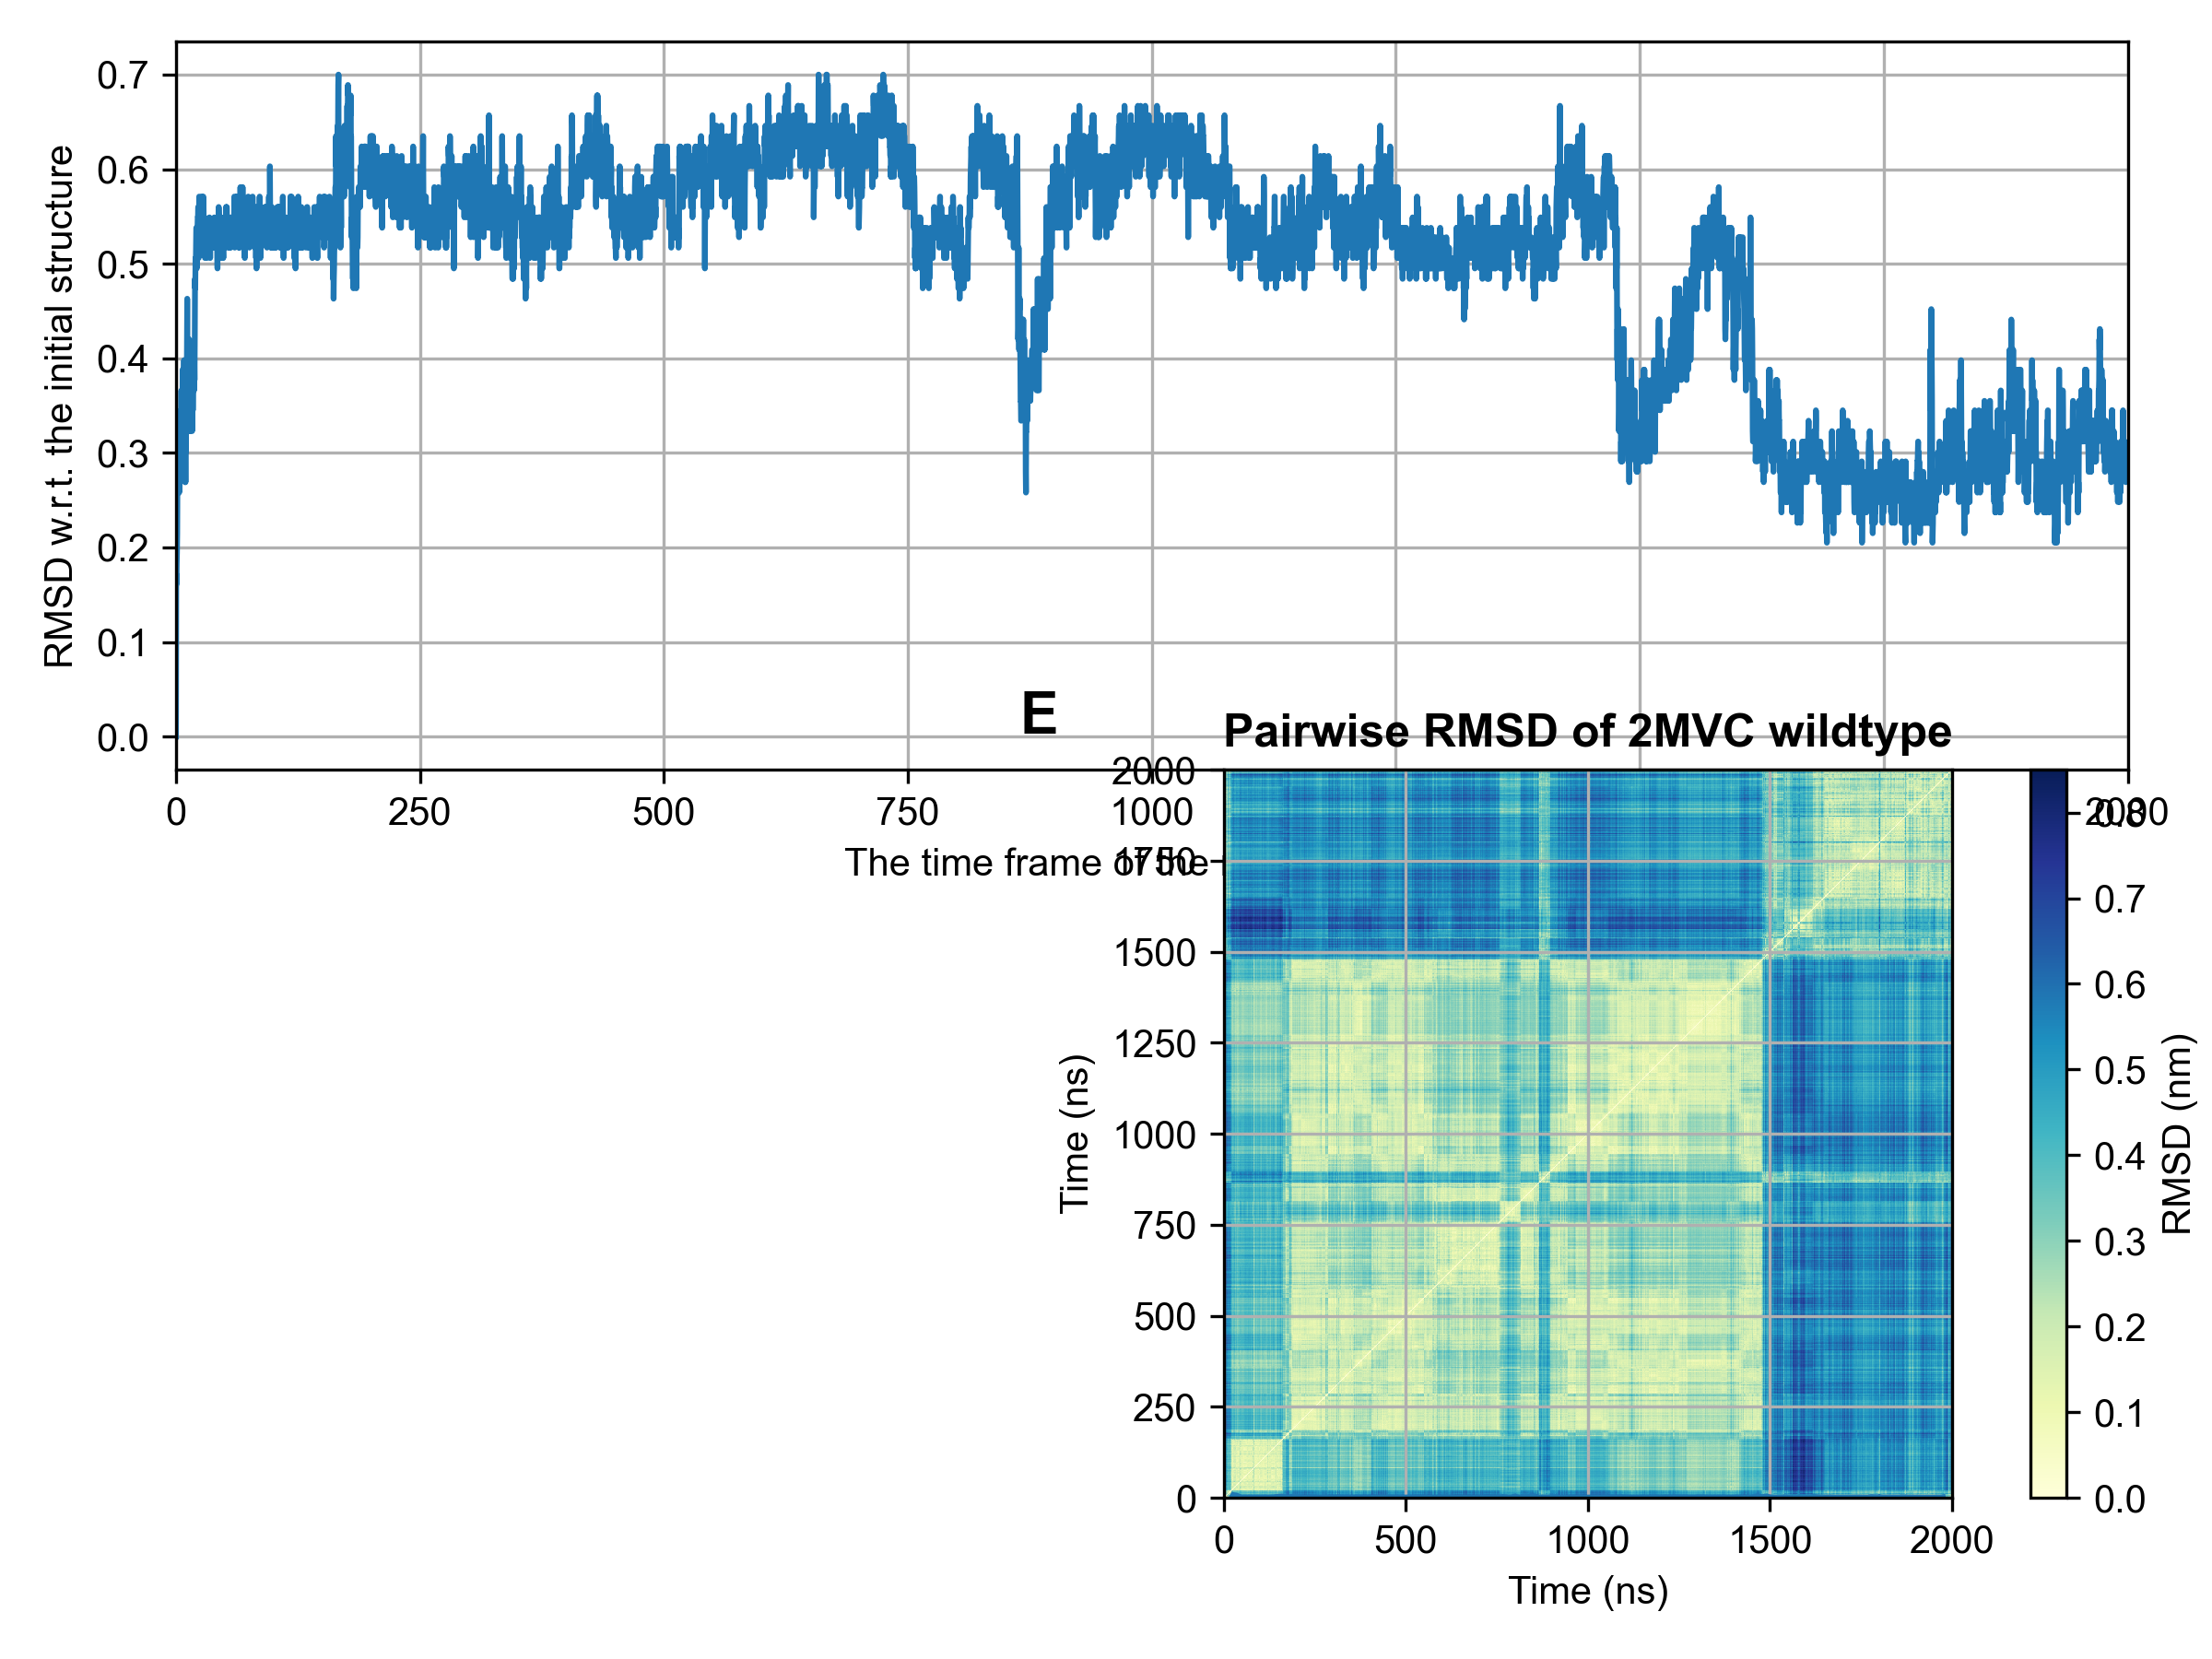
\includegraphics[width=\textwidth]{Figures/all_pairwise_rmsd.png}
\caption{The pairwise RMSD of calculated from the 250ps-spaced MD trajectory of each wild-type model, including 4EYD (A), 4EY9 (B), 4EY1 (C), 3I3Z (D), and 2MVC (E). As shown in the figure, the major transitions occur around 500--1500 ns, we therefore concluded that at least 2000 ns was required to sample the configurational ensemble of insulin.}
\label{supple_fig: pairwise_rmsd}
\end{figure}



\section{Metric distributions}
As supplemental statistics of our metrics, in Supplemental Figure \ref{SASA_distribution}, we provide the distributions of the SASA of the insulin scissile bonds and P1 sites. Note that we present kernel density estimation (KDE) ~\cite{davis2011remarks, parzen1962estimation} of the distributions instead of histograms so that the highly overlapped data would not obscure each other. In all the KDE plots, Scott's Rule ~\cite{scott2015multivariate} was used to automatically determine the smoothing bandwidth such that the KDE plots were visually consistent with the histograms of the data. As shown in the figure, the distributions of the scissile bond SASA all have multiple peaks, which reflects the fact that the SASA of the scissile bond is largely influenced by the orientation of the two adjacent residues. On the other hand, the two distributions of the P1 site SASA only have one peak. Importantly, in all metrics presented in the figure, GF 13 peaks at apparently lower SASA values compared to other variants, which is consistent with our finding mentioned in the main text that Metric 1 and Metric 2 had better predictiveness for the more proteolytically stable variants. Notably, we do not plot distributions for the other three metrics ($\beta$-sheet propensity, fraction of glycan-involved hydrogen bonds, and glycan-dimer occlusion fraction) presented in the main text because these metrics themselves are not time series but counts of occurrences. 

\renewcommand{\thefigure}{S\arabic{figure}}
\begin{figure}[H]
\centering
\includegraphics[width=\textwidth]{Figures/Fig_SASA_distribution.png}
\caption{The kernel density estimation (KDE) of distributions of the SASA at the scissile bonds and the P1 sites. (A) The distributions of the SASA at the scissile bonds between residues B25 and B26 and between residues B26 and B27. (B) The distributions of the SASA at the P1 sites, residues B24 and B25.}
\label{SASA_distribution}
\end{figure}

\section{Metric Correlations}
We examined the correlations between the 8 measures involved in the first 3 metrics for the proteolytic stability, which resulted in 28 combinations. (The 8 measures include scissile bond SASA of B25-B26 and B26-B27, residue SASA of B24 and B25, and $\beta$-sheet propensity of residues B22 to B25.) In the correlation plots in Figure \ref{corr_1} to Figure \ref{corr_3}, we annotated the Pearson correlation coefficients with its uncertainty estimated from bootstrapping where the bootstrap samples of both metric variables were drawn from values based on different wild-type models. We use Pearson correlation coefficients here by assuming a linear relationship between any two variables of interest. As a result, correlations between any two SASA measures (Figure \ref{corr_1}) tend to be stronger compared to the ones that involve at least one $\beta$-sheet propensity measure (Figure \ref{corr_2} and Figure \ref{corr_3}). This is expected because SASA measures are generally more predictive for the proteolytic stability than the $\beta$-sheet propensity measures. Correlating two measures that are highly associated with proteolytic stability naturally leads to a stronger correlation. The only exception is the correlation between $\beta$-sheet propensity of B22 and B23, which both are not predictive for the proteolytic stability but highly correlated with each other. This is probably because these two residues are adjacent to each other and contribute to similar secondary structures. 

\begin{figure}[H]
\centering
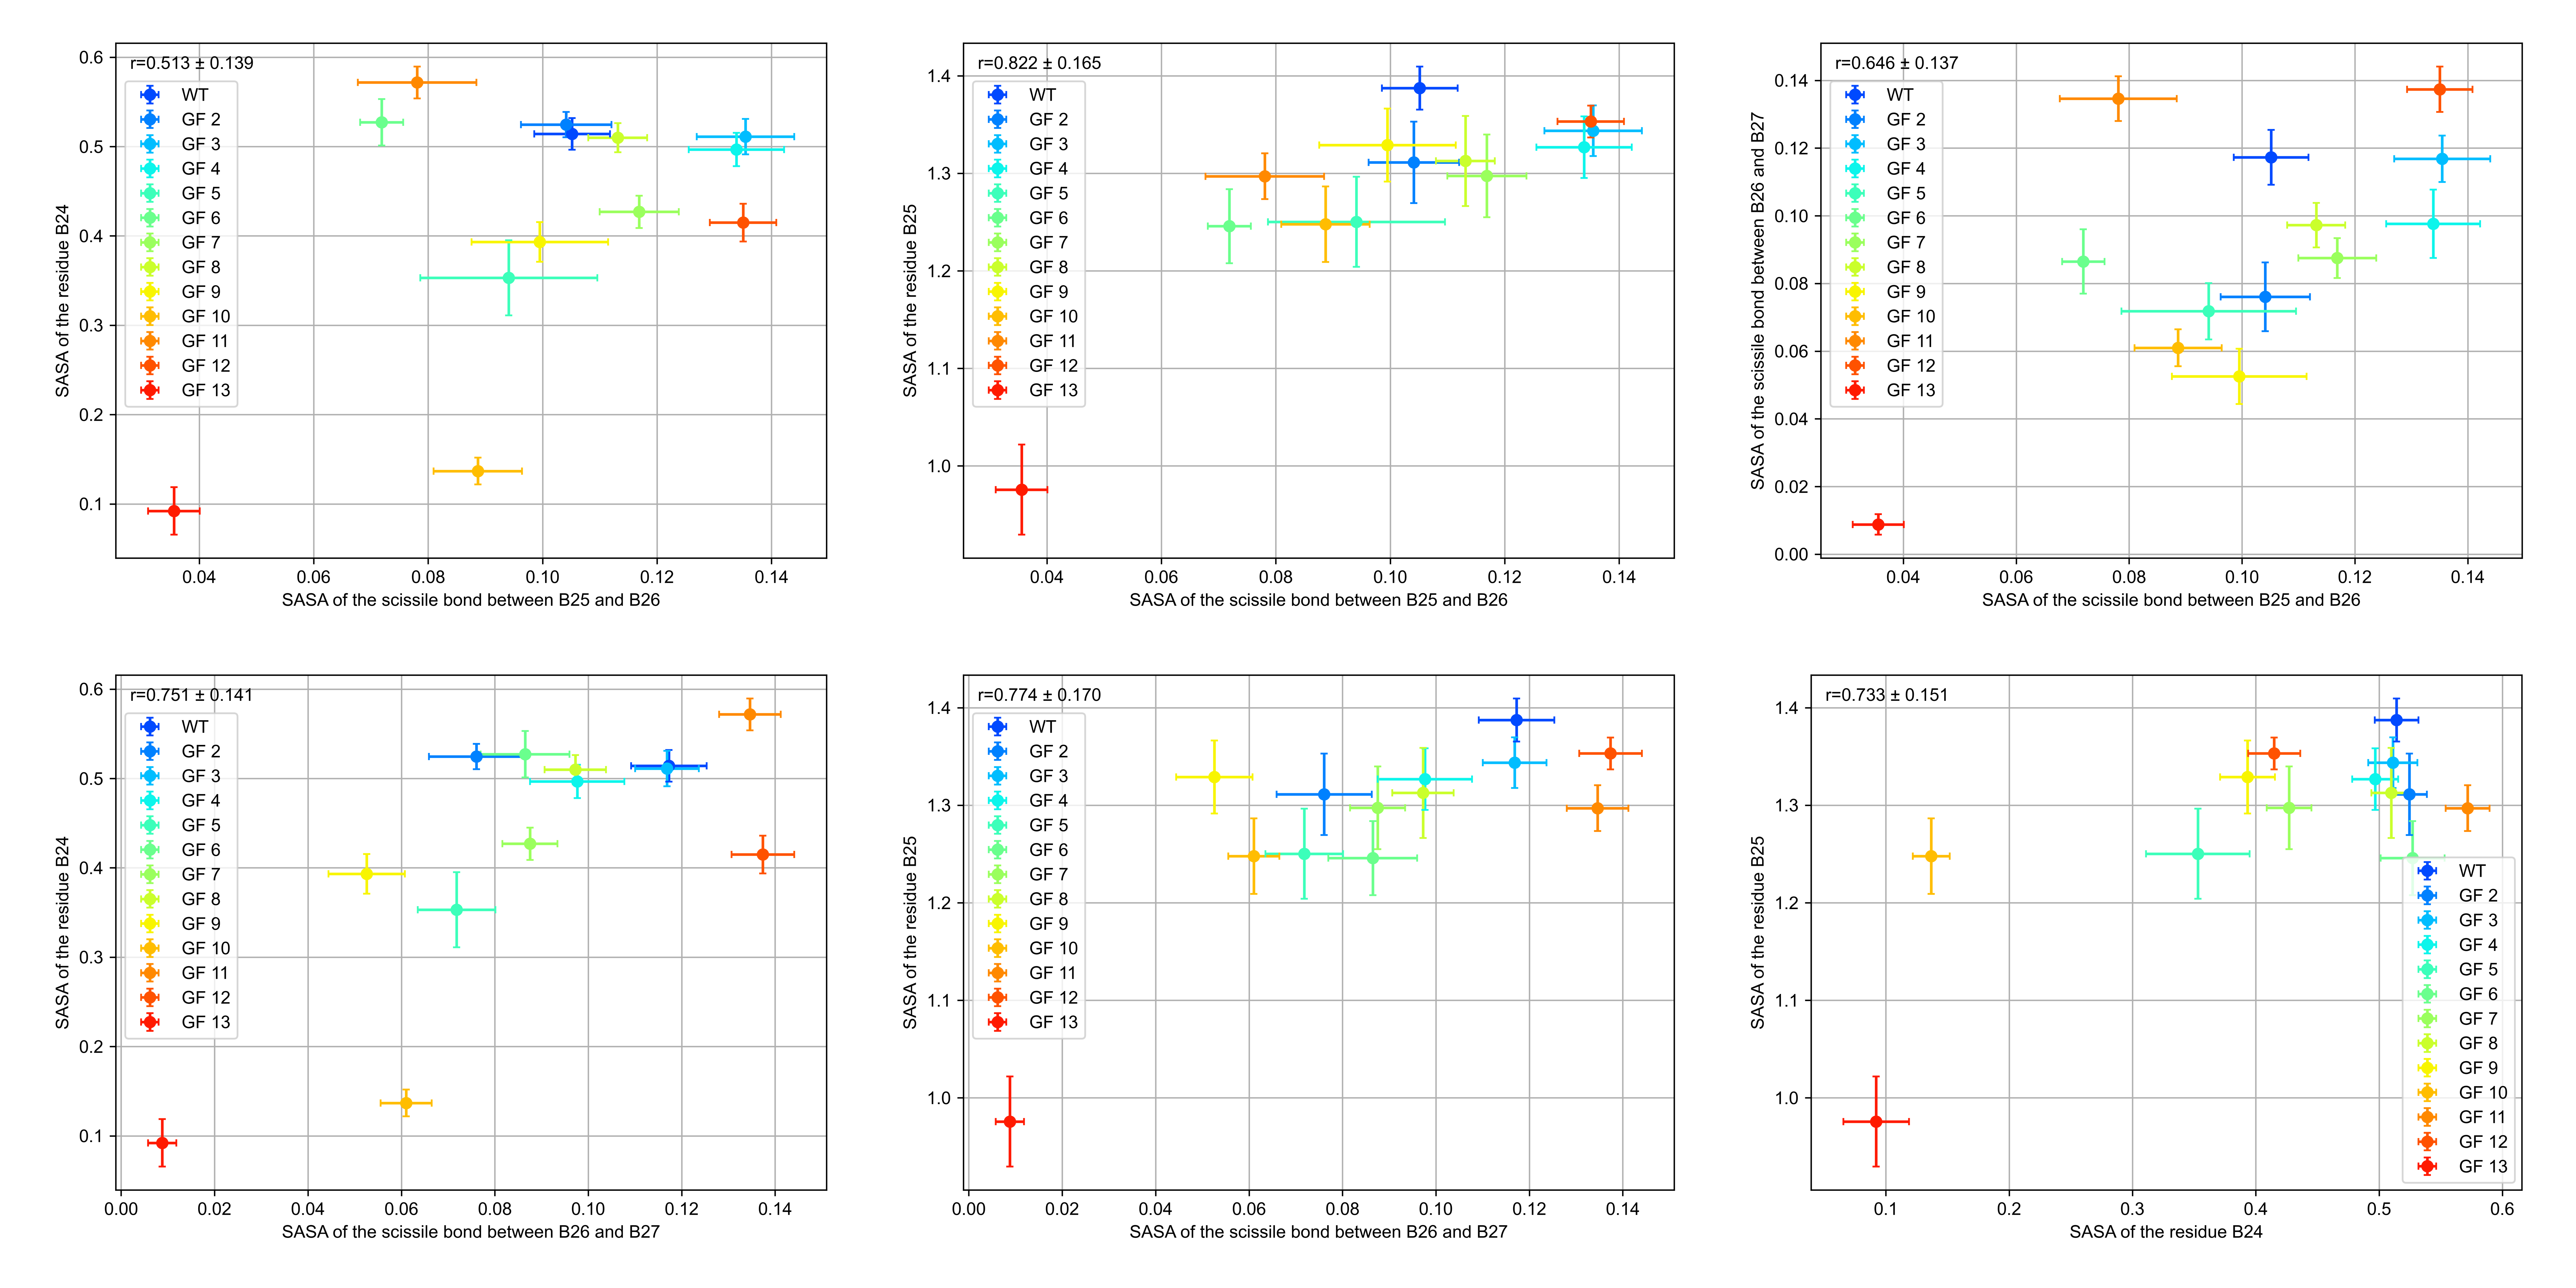
\includegraphics[width=0.95\textwidth]{Figures/Fig_SASA_metrics_correlation.png}
\caption{The correlation plots between any two SASA measures in Metric 1 and Metric 2 for the proteolytic stability. The Pearson correlation coefficients and their uncertainties determined from bootstrapping are annotated.}
\label{corr_1}
\end{figure}

\begin{figure}[H]
\centering
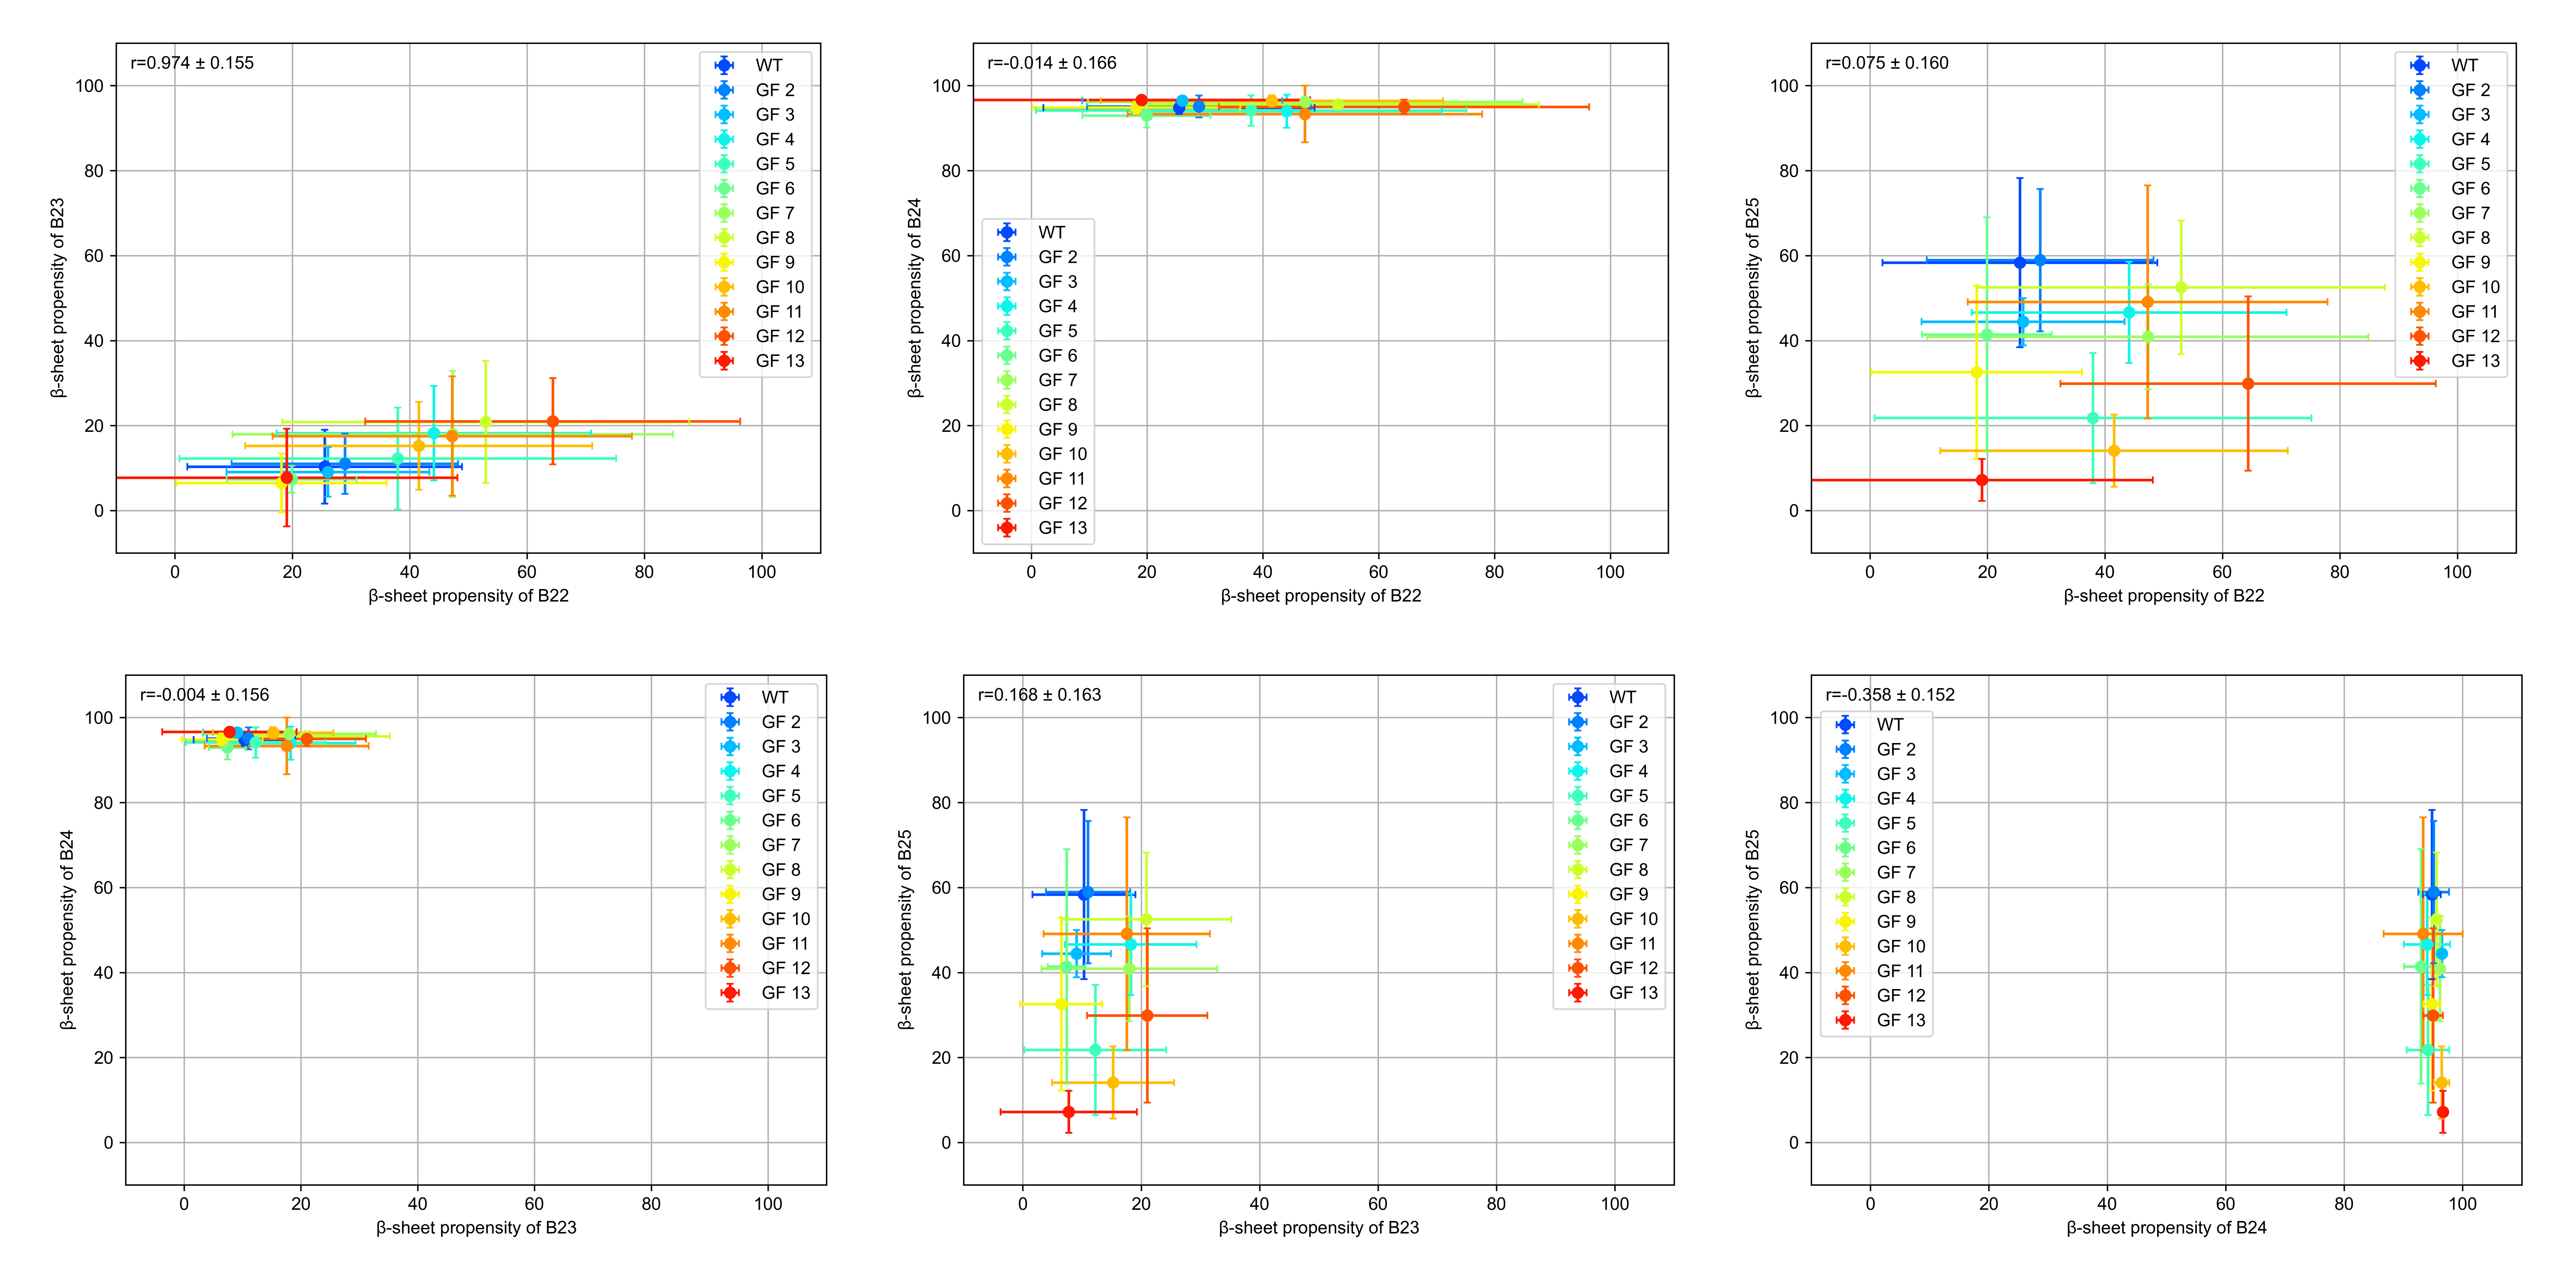
\includegraphics[width=0.95\textwidth]{Figures/Fig_beta_metrics_correlation.png}
\caption{The correlation plots between any two $\beta$-sheet propensity measures in Metric 3 for the proteolytic stability. The Pearson correlation coefficients and their uncertainties determined from bootstrapping are annotated.}
\label{corr_2}
\end{figure}

\begin{figure}[H]
\centering
\includegraphics[width=0.95\textwidth]{Figures/Fig_SASA_beta_metrics_correlation.png}
\caption{The correlation plots between any SASA measure in Metric 1 or Metric 2 and any $\beta$-sheet propensity measure in Metric 3 for the proteolytic stability. The Pearson correlation coefficients and their uncertainties determined from bootstrapping are annotated.}
\label{corr_3}
\end{figure}


\section{Additional Tables}

\renewcommand{\thetable}{S\arabic{table}}
\begin{table}[ht]
\begin{minipage}{\textwidth}
\caption{Comparison of histidine protonation states of wild-type structures with the range of input pH values to H++ consistent with this protonation. Note that the pH ranges corresponding to the fixed total charges of -1 could vary between different models, since pH values from H++ are only approximations based on a single input structure, instead of the entire ensemble.}
\label{supple_tab: protonation}
\centering
\begin{tabular}{@{}cccccc@{}}

\toprule
     & 4EYD & 4EY1 & 3I3Z & 4EY9 & 2MVC \\
\midrule
Total charges & -1 & -1 & -1 & -1 & -1 \\
pH value & 6.9-7.8 & 6.9-7.8 & 6.6-6.9 & 7.7-7.9 & 6.5-7.3 \\
HisB5 & HIP (+1) &HIP (+1) &HIP (+1) &HIP (+1) & HIE (+0) \\
HisB10 & HIE (+0) & HIE (+0) &HIE (+0) &HID (+0) & HIP (+1)  \\
\botrule
\end{tabular}
\end{minipage}
\end{table}


\renewcommand{\thetable}{S\arabic{table}}
\begin{table}[ht]
\caption{Dimer occlusion autocorrelation lag times for each of the listed models. All numbers are listed in units of nanoseconds.}
\centering
\begin{adjustbox}{width=1\textwidth,center=\textwidth}
\begin{tabular}{@{}ccccccccccccc@{}}
\toprule
&GF 2&GF 3&GF 4&GF 5&GF 6&GF 7&GF 8&GF 9&GF 10&GF 11&GF 12&GF 13\\ \midrule
4EYD&NA& NA&3.45&63.56&69.11& NA&NA&45.79&121.70&21.65&140.40&24.77 \\ %\hline
4EY1&NA& NA&6.89&371.83&71.04& NA&19.37&205.24&159.14&58.17&360.45&637.20 \\ %\hline
4EY9&NA & NA &18.53&274.66&97.34& NA &NA &12.55&496.98&0.39&89.13&57.77 \\ %\hline
3I3Z&NA & NA &93.49&62.86&199.65& NA & NA &45.27&62.80&42.78&97.81&281.52 \\ %\hline
2MVC&3.98&NA &21.31&54.78&105.28&NA &NA &114.61&59.62&58.75&66.00&81.57 \\ \botrule
\end{tabular}
\end{adjustbox}
\label{supple_tab: occlusion_lag}
\end{table}

\begin{table}[ht]
\caption{The glycan-involved hydrogen bonds and their existence percentages of each glycoform.}
\begin{adjustbox}{width=1\textwidth}
\begin{tabular}{@{}cccccc@{}}
\toprule
\# & 4EYD-based GFs                                                                                                                             & 4EY1-based GFs                                                                                                                                                             & 4EY9-based GFs                                                                                                                                                             & 3I3Z-based GFs                                                                                                                            & 2MVC-based GFs                                                                                                                            \\ \midrule
1  & N/A                                                                                                                                        & N/A                                                                                                                                                                        & N/A                                                                                                                                                                        & N/A                                                                                                                                       & N/A                                                                                                                                       \\ \midrule
2  & None                                                                                                                                       & ThrA8(OG1)-GalNAc{[}1{]}(O2N):10\%                                                                                                                                         & None                                                                                                                                                                       & None                                                                                                                                      & \begin{tabular}[c]{@{}c@{}}GlnA5(NE2)-GalNAc{[}1{]}(O6): 14\%\\ GlnA15(NE2)-GalNAc{[}1{]}(O6): 13\%\end{tabular}                          \\ \midrule
3  & None                                                                                                                                       & None                                                                                                                                                                       & None                                                                                                                                                                       & None                                                                                                                                      & GlnA15(NE2)-52(O2N):11\%                                                                                                                  \\ \midrule
4  & None                                                                                                                                       & None                                                                                                                                                                       & None                                                                                                                                                                       & None                                                                                                                                      & None                                                                                                                                      \\ \midrule
5  & None                                                                                                                                       & \begin{tabular}[c]{@{}c@{}}PheB24(N)-GalNAc{[}1{]}(O3): 48\%\\ ThrB30(N)-GalNAc{[}1{]}(O2N): 16\%\end{tabular}                                                             & PheB24(N)-GalNAc{[}1{]}(O3): 11\%                                                                                                                                          & \begin{tabular}[c]{@{}c@{}}ThrB27(N)-GalNAc{[}1{]}(O3):15\%\\ Glu4(N)-GalNAc{[}1{]}(O2N): 14\%\end{tabular}                               & PheB24(N)-GalNAc{[}1{]}(O3): 10\%                                                                                                         \\ \midrule
6  & ThrB27(N)-GalNAc{[}1{]}(O3):26\%                                                                                                           & ThrB27(N)-GalNAc(1)(O3):26\%                                                                                                                                               & None                                                                                                                                                                       & None                                                                                                                                      & \begin{tabular}[c]{@{}c@{}}CysA7(N)-GalNAc{[}1{]}(O2N): 18\%\\ ThrB27(N)-GalNAc(1)(O3): 12\%\end{tabular}                                 \\ \midrule
7  & None                                                                                                                                       & None                                                                                                                                                                       & None                                                                                                                                                                       & None                                                                                                                                      & GlnA15(NE2)-Man{[}1{]}(O4): 18\%                                                                                                          \\ \midrule
8  & GlnA5(NE2)-Man{[}2{]}(O2): 12\%                                                                                                            & GlnA5(NE2)-Man{[}2{]}(O2): 11\%                                                                                                                                            & None                                                                                                                                                                       & GlnA5(NE2)-Man{[}1{]}(O5): 12\%                                                                                                           & None                                                                                                                                      \\ \midrule
9  & \begin{tabular}[c]{@{}c@{}}PheB24(N)-Man{[}1{]}(O3): 22\%\\ TyrB16(OH)-Man{[}1{]}(O4): 13\%\end{tabular}                                   & None                                                                                                                                                                       & \begin{tabular}[c]{@{}c@{}}PheB24(N)-Man{[}1{]}(O3): 27\%\\ TyrB16(OH)-Man{[}1{]}(O4): 19\%\end{tabular}                                                                   & None                                                                                                                                      & None                                                                                                                                      \\ \midrule
10 & \begin{tabular}[c]{@{}c@{}}PheB24(N)-Man{[}1{]}(O3): 52\%\\ ThrB30(N)--Man{[}2{]}(O2): 35\%\\ ThrB27(N)--Man{[}2{]}(O6): 23\%\end{tabular} & \begin{tabular}[c]{@{}c@{}}ThrB27(N)-Man{[}2{]}(O6): 46\%\\ PheB24(N)-Man{[}1{]}(O3): 30\%\\ TyrB16(OH)-Man{[}1{]}(O4): 15\%\end{tabular}                                  & \begin{tabular}[c]{@{}c@{}}ThrB27(N)-Man{[}2{]}(O6): 45\%\\ PheB24(N)-Man{[}1{]}(O3): 28\%\\ TyrB16(OH)-Man{[}1{]}(O4): 11\%\end{tabular}                                  & \begin{tabular}[c]{@{}c@{}}ThrB27(N)-Man{[}2{]}(O6): 47\%\\ PheB24(N)-Man{[}1{]}(O3): 15\%\end{tabular}                                   & \begin{tabular}[c]{@{}c@{}}ThrB27(N)-Man{[}2{]}(O6): 47\%\\ PheB24(N)-Man{[}1{]}(O3): 37\%\\ TyrB16(OH)-Man{[}1{]}(O4): 14\%\end{tabular} \\ \midrule
11 & None                                                                                                                                       & None                                                                                                                                                                       & None                                                                                                                                                                       & None                                                                                                                                      & None                                                                                                                                      \\ \midrule
12 & \begin{tabular}[c]{@{}c@{}}ThrB30(N)-Man{[}2{]}(O6): 31\%\\ GlyB23(N)-Man{[}1{]}(O3): 10\%\end{tabular}                                    & \begin{tabular}[c]{@{}c@{}}TyrA19(OH)-Man{[}1{]}(O4): 51\%\\ ThrB27(N)-Man{[}1{]}(O3): 43\%\\ ThrB30(N)-Man{[}2{]}(O6): 19\%\end{tabular}                                  & \begin{tabular}[c]{@{}c@{}}ThrB30(N)-Man{[}2{]}(O6): 24\%\\ ValA3(N)-Man{[}2{]}(O2): 15\%\end{tabular}                                                                     & ThrB30(N)--Man{[}2{]}(O6): 38\%                                                                                                           & \begin{tabular}[c]{@{}c@{}}ThrB30(N)-Man{[}2{]}(O6): 49\%\\ GlyB8(N)-Man{[}2{]}(O4): 10\%\end{tabular}                                    \\ \midrule
13 & \begin{tabular}[c]{@{}c@{}}ThrB27(N)-Man{[}2{]}(O6): 61\%\\ PheB24(N)-Man{[}1{]}(O3): 49\%\\ TyrB16(OH)-Man{[}1{]}(O4): 16\%\end{tabular}  & \begin{tabular}[c]{@{}c@{}}ThrB27(N)-Man{[}2{]}(O6): 31\%\\ ThrB27(N)-Man{[}3{]}(O6): 14\%\\ PheB24(N)-Man{[}1{]}(O3): 12\%\\ TyrB16(OH)-Man{[}1{]}(O4): 11\%\end{tabular} & \begin{tabular}[c]{@{}c@{}}ThrB27(N)-Man{[}2{]}(O6): 27\%\\ PheB24(N)-Man{[}1{]}(O3): 17\%\\ ThrB27(N)-Man{[}3{]}(O6): 15\%\\ TyrB16(OH)-Man{[}1{]}(O4): 10\%\end{tabular} & \begin{tabular}[c]{@{}c@{}}ThrB27(N)-Man{[}2{]}(O6): 43\%\\ PheB24(N)-Man{[}1{]}(O3): 25\%\\ TyrB16(OH)-Man{[}1{]}(O4): 12\%\end{tabular} & \begin{tabular}[c]{@{}c@{}}ThrB27(N)-Man{[}2{]}(O6): 44\%\\ PheB24(N)-Man{[}1{]}(O3): 22\%\end{tabular}                                   \\ \botrule
\end{tabular}
\end{adjustbox}
\label{supple_tab: hbond}
\end{table}

% atom type table
\begin{table}[ht]
\caption{The atom types involved in the glycan-involved hydrogen bonds.}
\label{supple_tab: atom_types}
\centering
\begin{tabular}{@{}ccc@{}}
\toprule
Atom type & Role     & Description                                                      \\ \midrule
N         & Donor    & An sp$^{2}$ nitrogen in amide group                              \\ %\hline
NE2       & Donor    & An epsilon nitrogen.                                             \\ %\hline
OH        & Donor    & An alcohol oxygen in Tyr                                        \\ %\hline
OG1       & Donor    & An alcohol oxygen in Thr                                        \\ %\hline
O2        & Acceptor & The oxygen atom connected to the second carbon atom of the sugar \\ %\hline
O3        & Acceptor & The oxygen atom connected to the third carbon atom of the sugar  \\ %\hline
O4        & Acceptor & The oxygen atom connected to the fourth carbon atom of the sugar \\ %\hline
O5        & Acceptor & The oxygen atom connected to the fifth carbon atom of the sugar  \\ %\hline
O6        & Acceptor & The oxygen atom connected to the sixth carbon atom of the sugar  \\ %\hline
O2N       & Acceptor & The oxygen atom of the N-acetyl group                            \\ \botrule
\end{tabular}
\end{table}

%%%%% Occlusion results table
\renewcommand{\thetable}{S\arabic{table}}
\begin{table}[ht]
\caption{Glycoforms ordered from most to least proportion occlusion, based on proportion of simulation with measured occlusion.}
\label{supple_tab: occlusion_tab}
\centering
%\begin{adjustbox}{width=0.9\textwidth,center=\textwidth}
%\small
\begin{tabular} {|l| c c c c c c c c c c c c|}
    \hline
     & \multicolumn{4}{c}{\textit{least occlusion}} &&& & & \multicolumn{4}{c|}{\textit{most occlusion}}\\
    \hline     
    4EYD&2&3&7&8&4&11&12&6&\textbf{9}&\textbf{10}&5&\textbf{13}\\
    4EY1&2&3&7&8&4&11&6&12&\textbf{9}&\textbf{10}&5&\textbf{13}\\
    4EY9&2&3&7&8&11&4&6&12&5&\textbf{9}&\textbf{10}&\textbf{13}\\
    3I3Z&2&3&7&8&4&6&11&12&\textbf{9}&5&\textbf{13}&\textbf{10}\\
    2MVC&3&7&8&2&4&11&6&12&\textbf{9}&5&\textbf{10}&\textbf{13}\\
    \hline
    & \multicolumn{4}{c|}{\textit{low batch}} & \multicolumn{4}{c|}{\textit{medium batch}} & \multicolumn{4}{c|}{\textit{high batch}}\\
    \hline
\end{tabular}
%\end{adjustbox}
\end{table}

\section{Additional Figures}
\renewcommand{\thefigure}{S\arabic{figure}}
\begin{figure}[H]
\centering
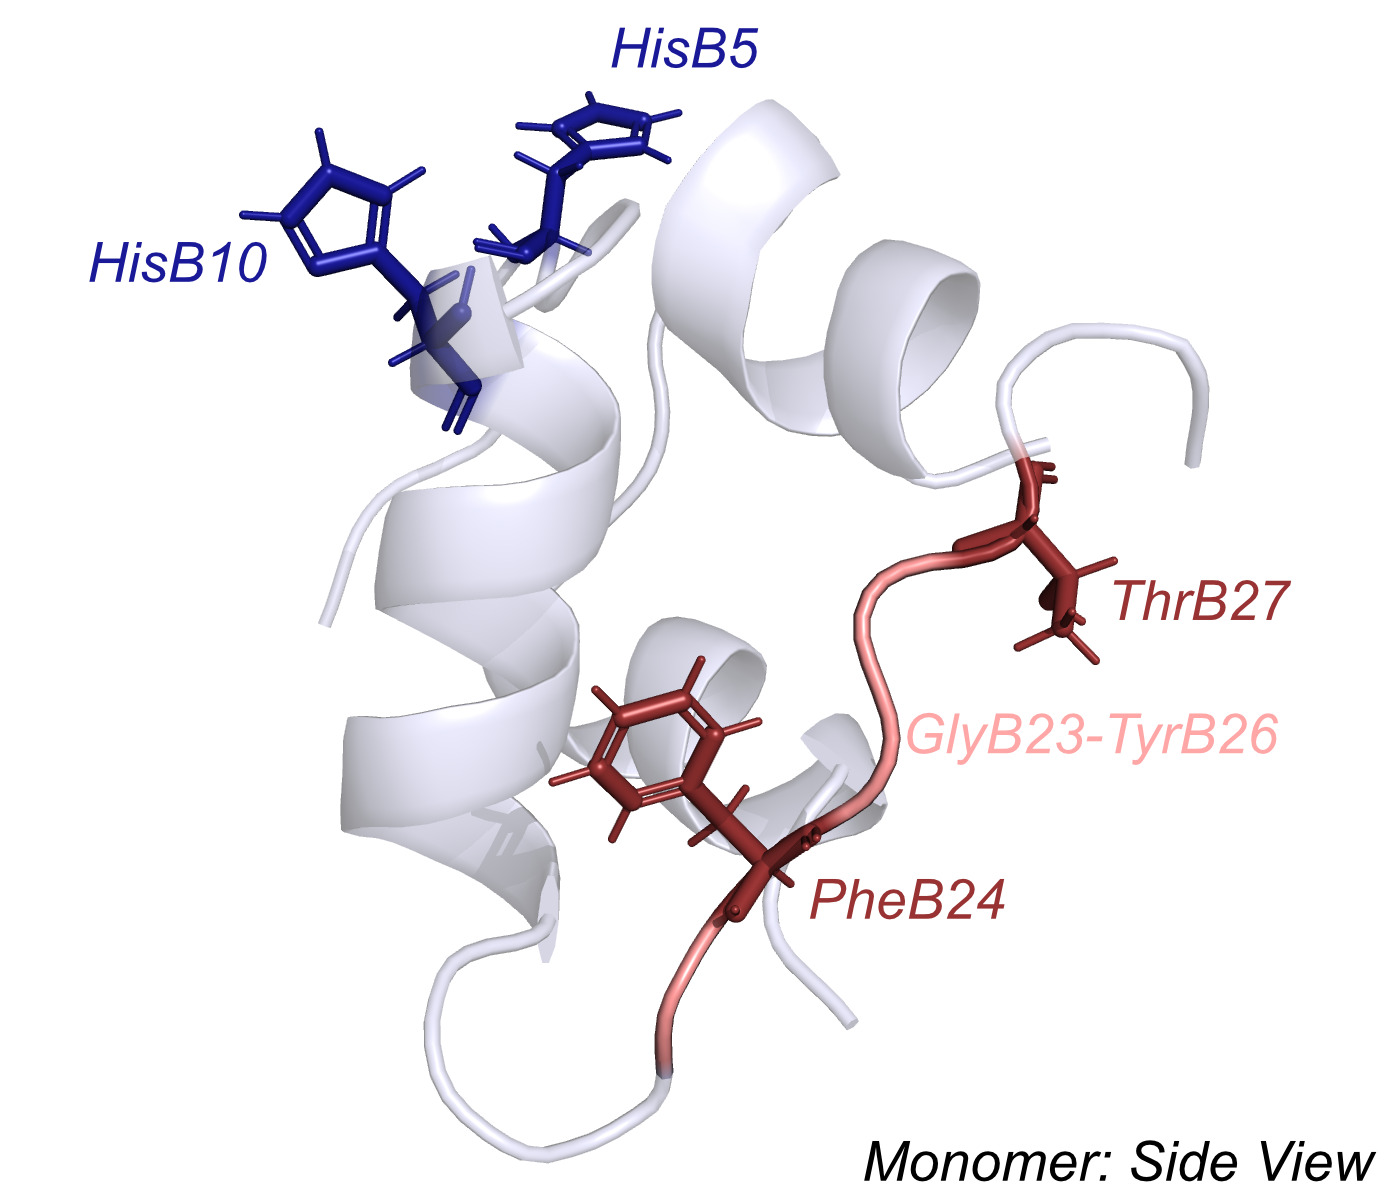
\includegraphics[width=0.6\textwidth]{Figures/Fig_histidine_WT.png}
\caption{The histidine residues (HisB5, and HisB10, colored in blue) are shown with residues PheB24 and ThrB27 (colored red) which are important in enhancing proteolytic stability and residues GlyB23-TyrB26 (colored salmon), important in determining dimerization potential.}
\label{supple_fig: WT_hist}
\end{figure}

\renewcommand{\thefigure}{S\arabic{figure}}
\begin{figure}[H]
\centering
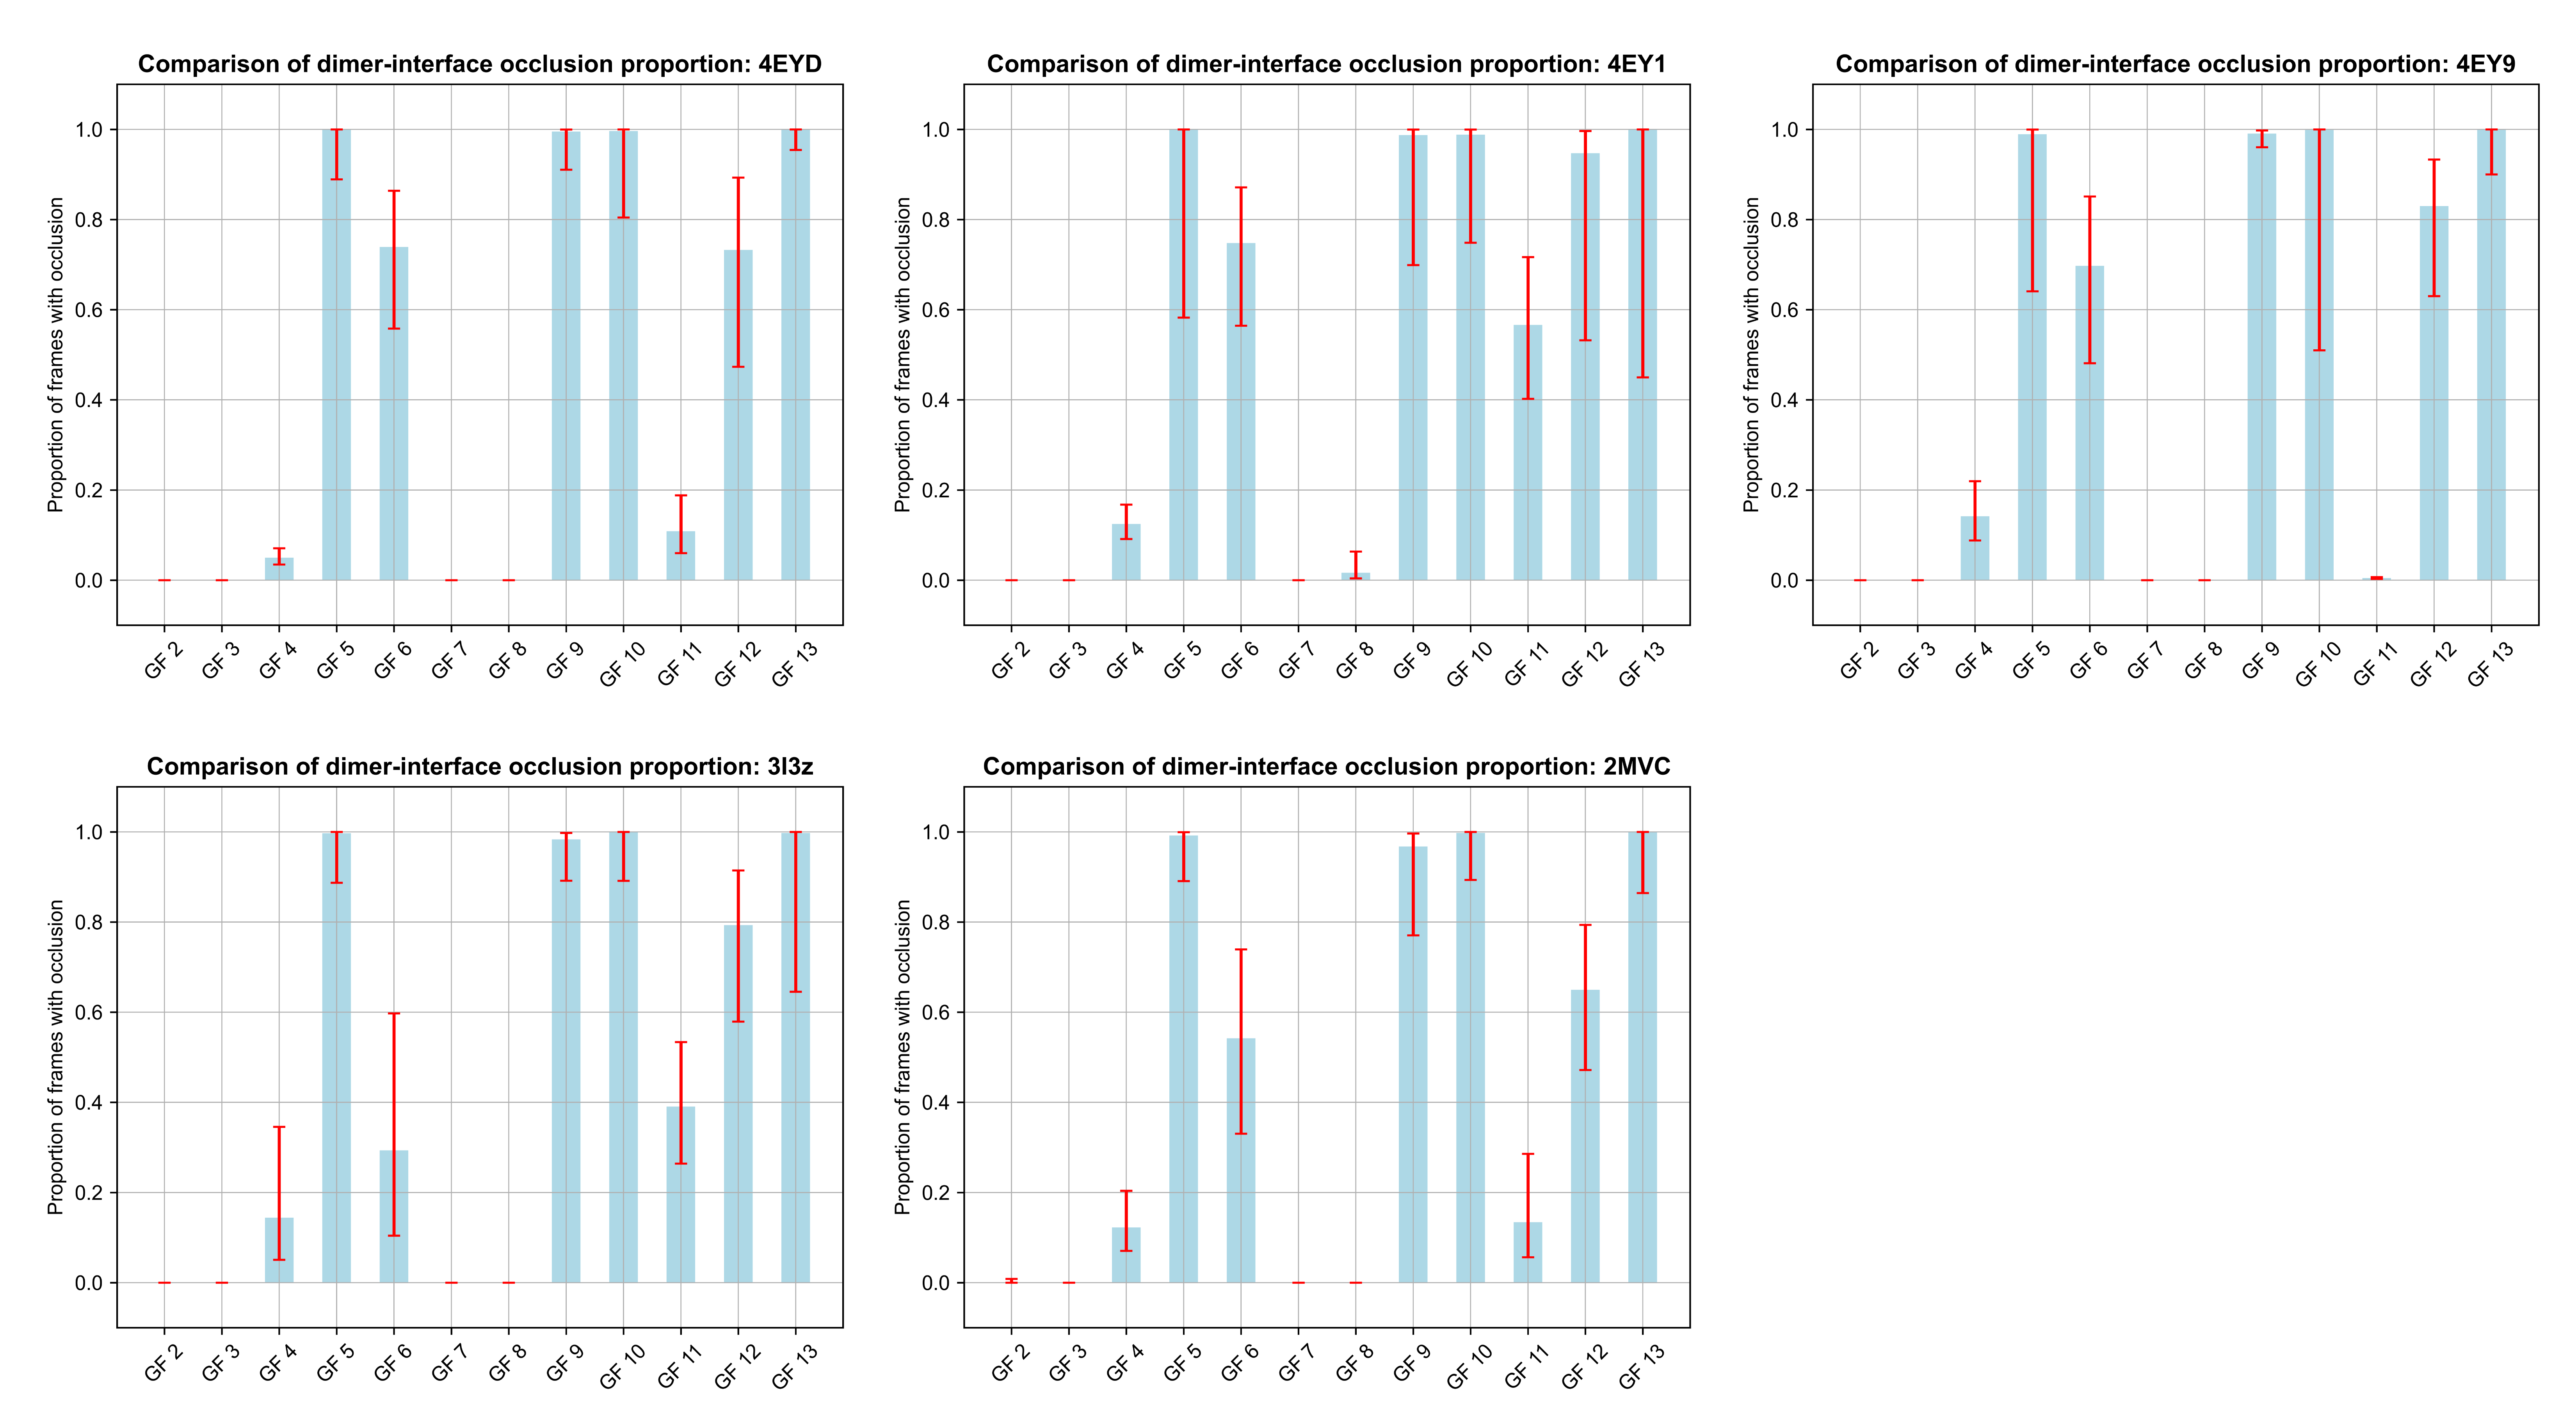
\includegraphics[width=1.0\textwidth]{Figures/occlusion_proportion_models_2.png}
\caption{Proportion of frames with glycan-dimer occlusion for each glycoform. Red bars represent the asymmetric 95\% Wilson score confidence interval.}
\label{supple_fig: occlusion_binomial}
\end{figure}

\renewcommand{\thefigure}{S\arabic{figure}}
\begin{figure}[H]
\centering
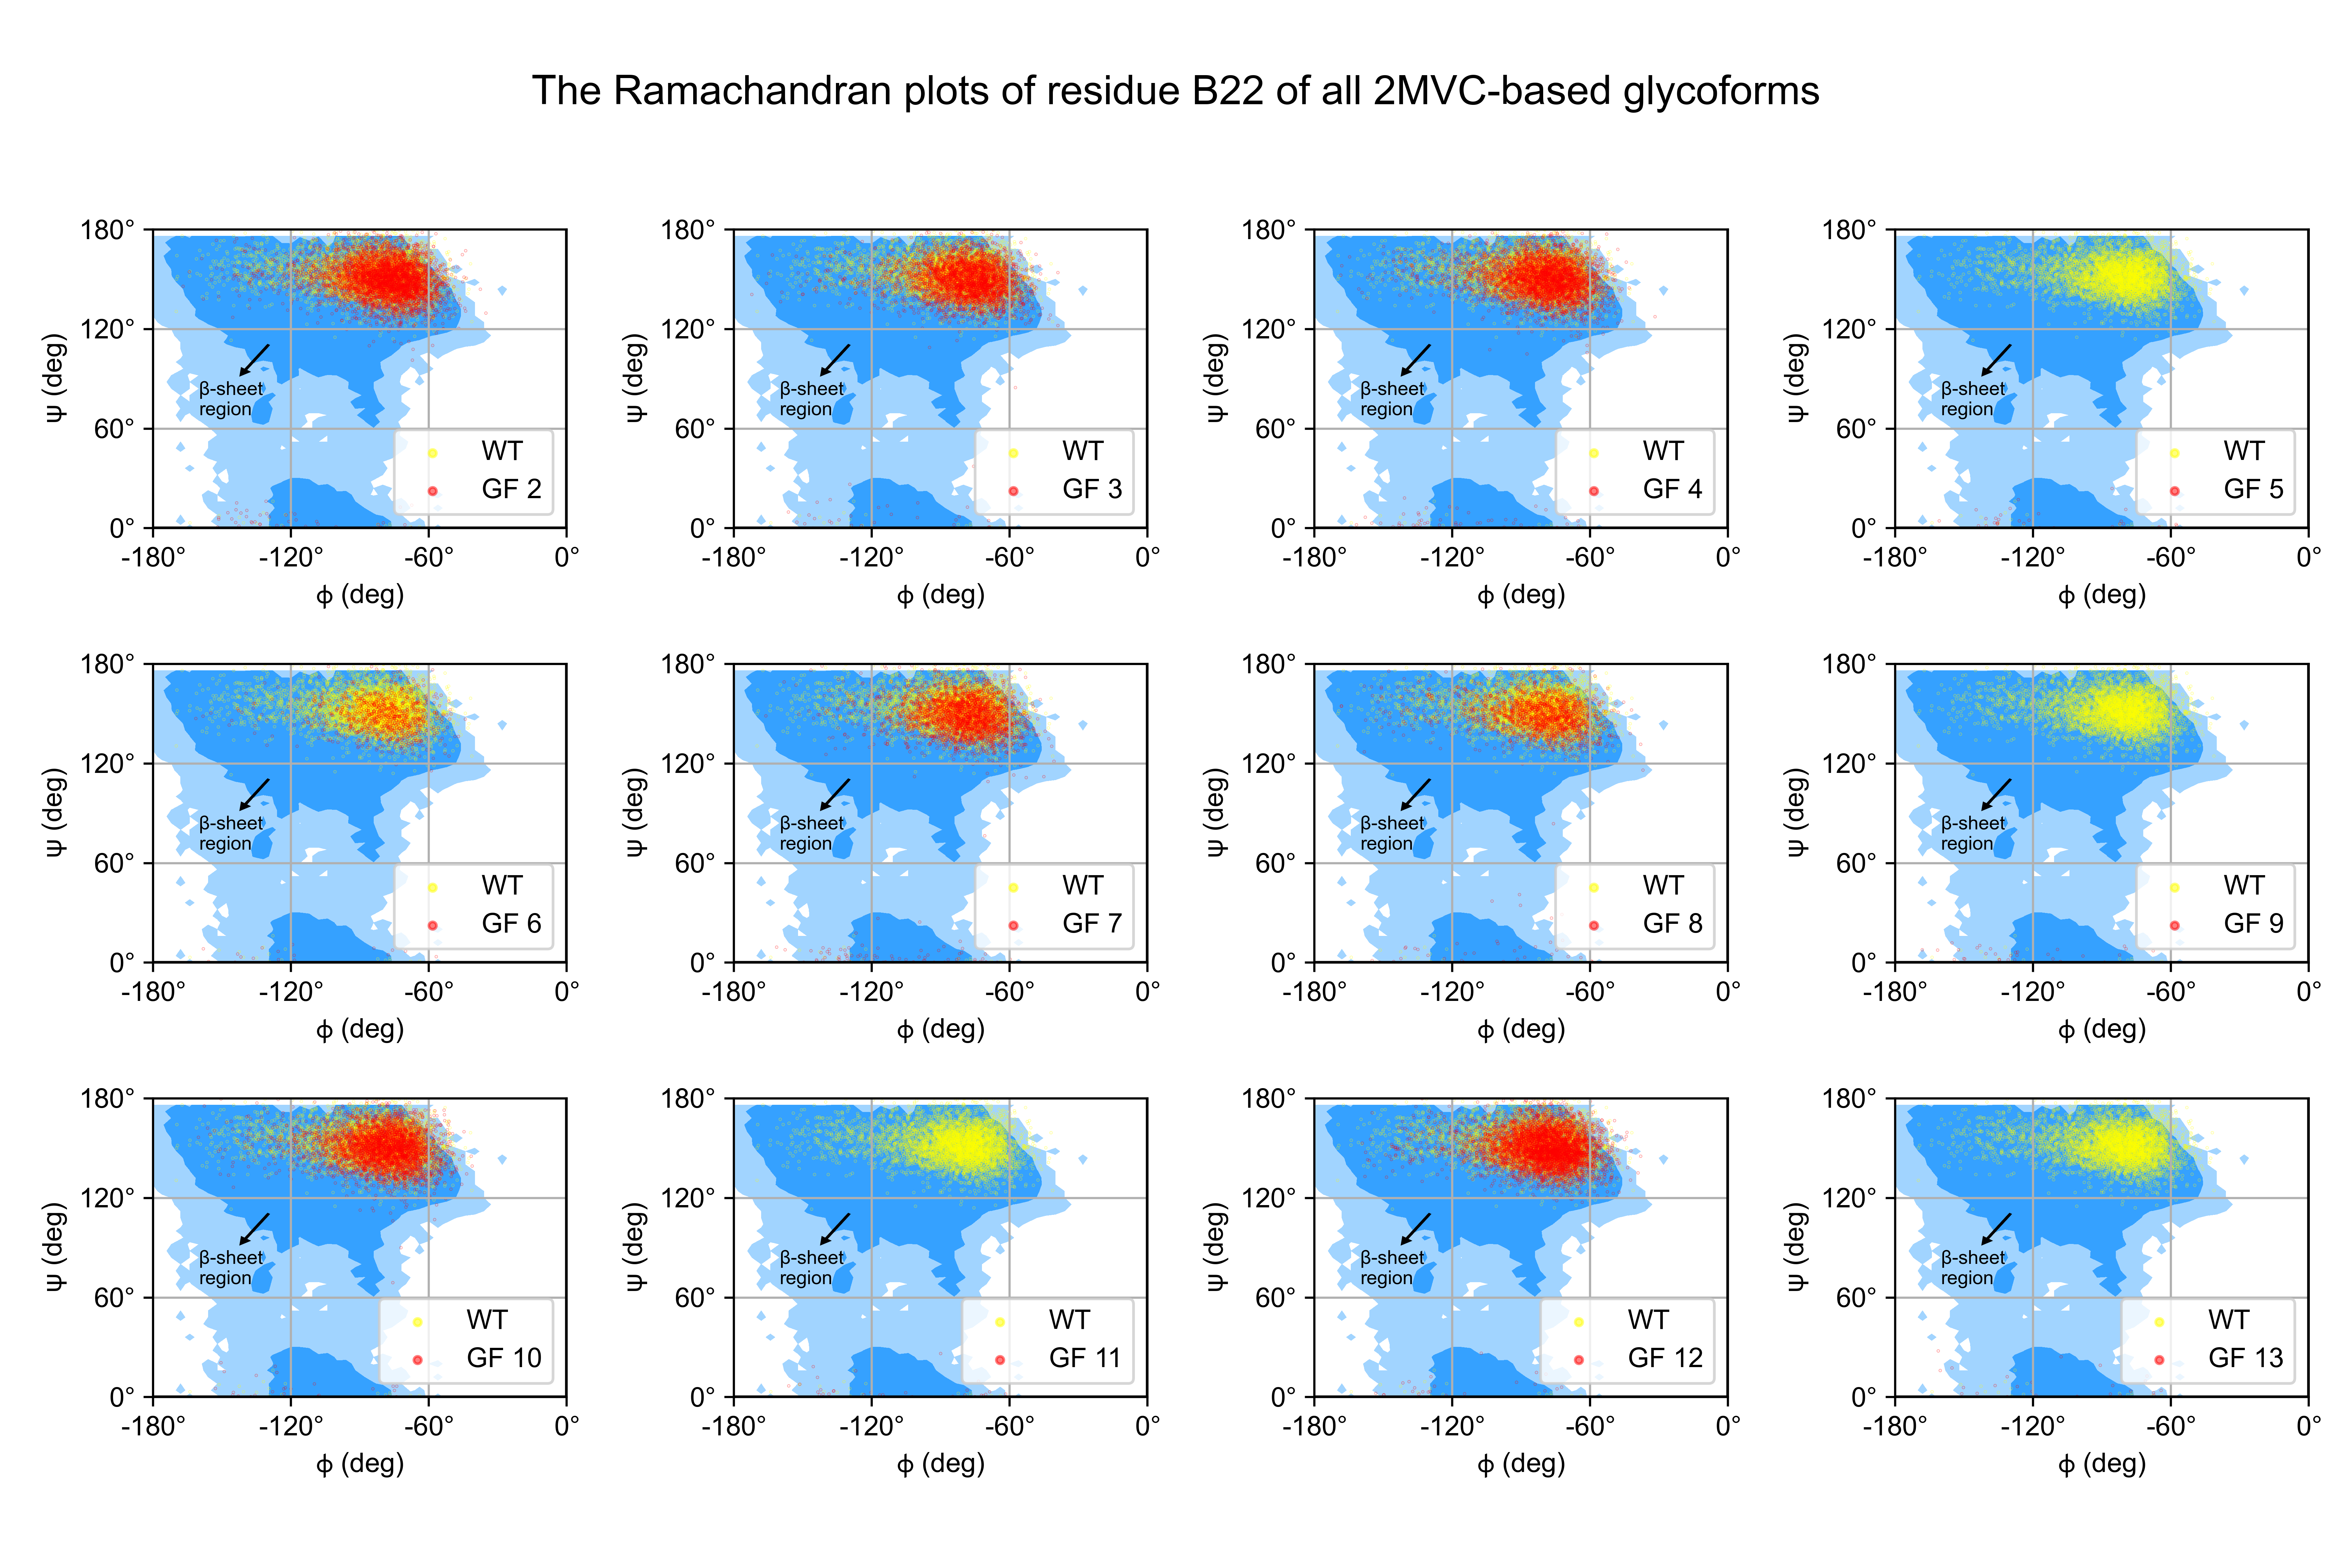
\includegraphics[width=\textwidth]{Figures/2MVC_multi_rama_plot_res_43.png}
\caption{The Ramachandran plots of residue B22 of all 2MVC-based glycoforms. The contours in the background show the allowed region in the second quadrant where the dihedral angles can reside. The deeper blue region is the $\beta$-sheet region defined by Lovell et al~\cite{lovell2003structure}.}
\end{figure}

\renewcommand{\thefigure}{S\arabic{figure}}
\begin{figure}[H]
\centering
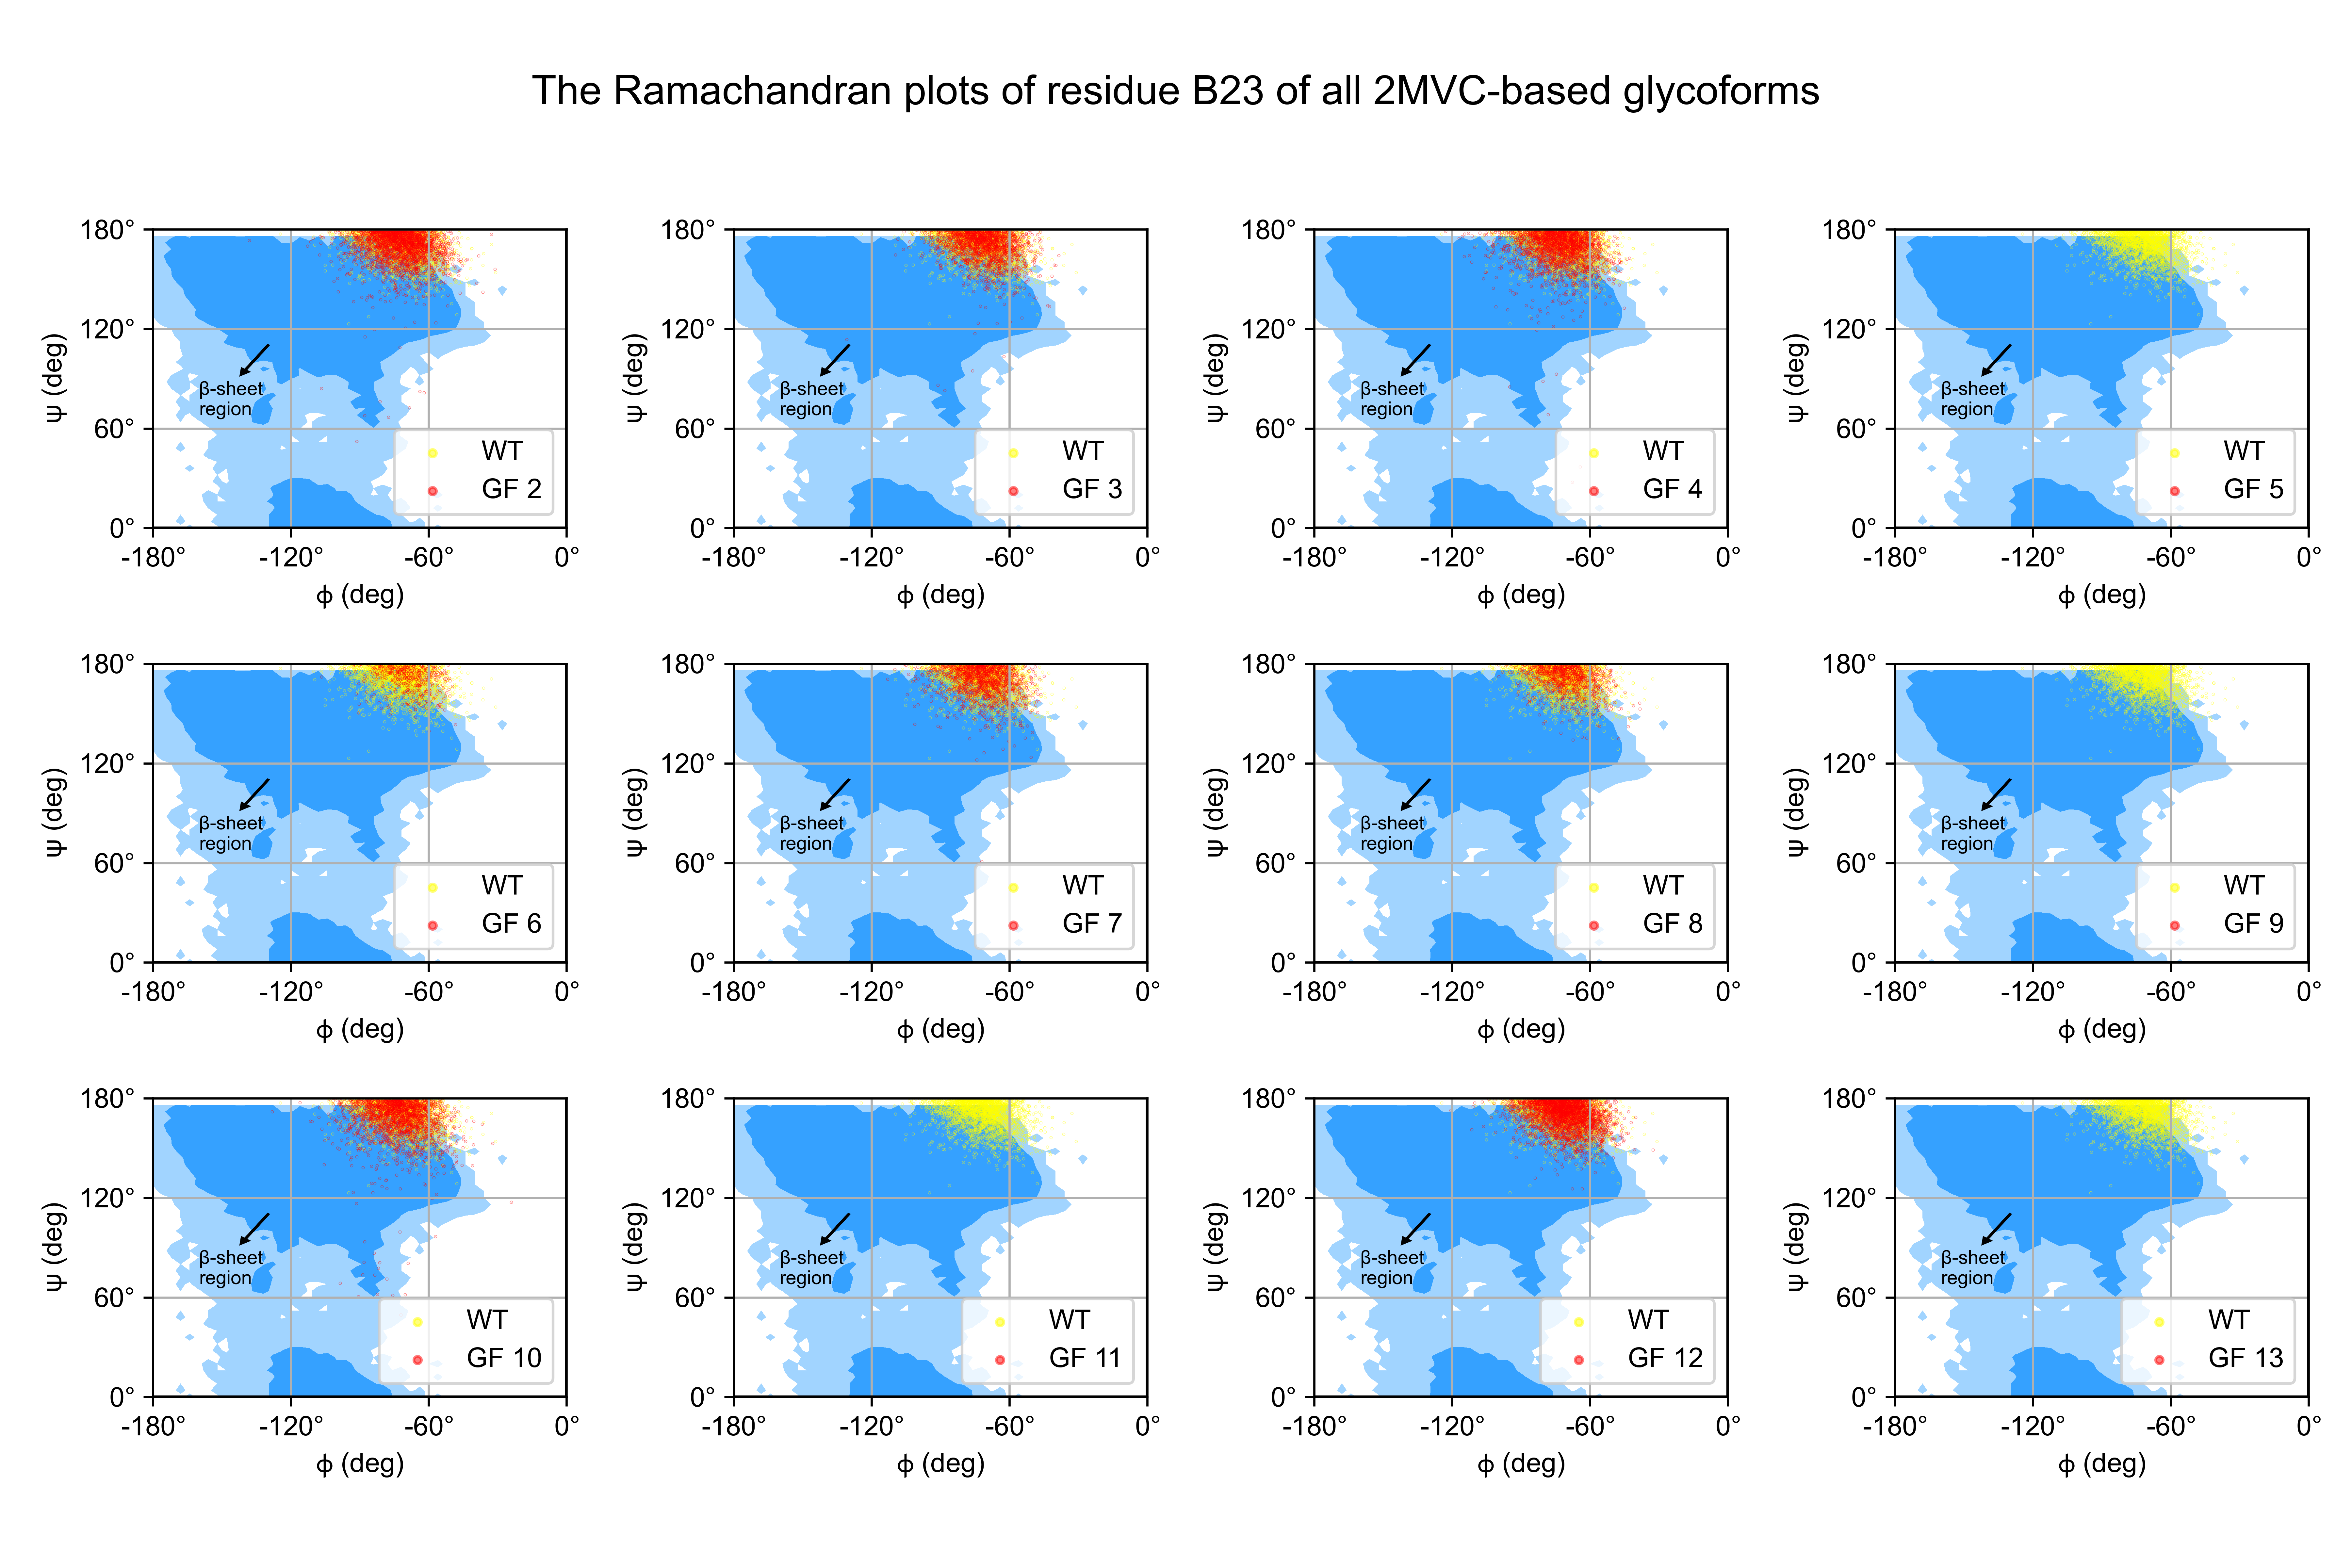
\includegraphics[width=\textwidth]{Figures/2MVC_multi_rama_plot_res_44.png}
\caption{The Ramachandran plots of residue B23 of all 2MVC-based glycoforms. The contours in the background show the allowed region in the second quadrant where the dihedral angles can reside. The deeper blue region is the $\beta$-sheet region defined by Lovell et al~\cite{lovell2003structure}.}
\end{figure}

\renewcommand{\thefigure}{S\arabic{figure}}
\begin{figure}[H]
\centering
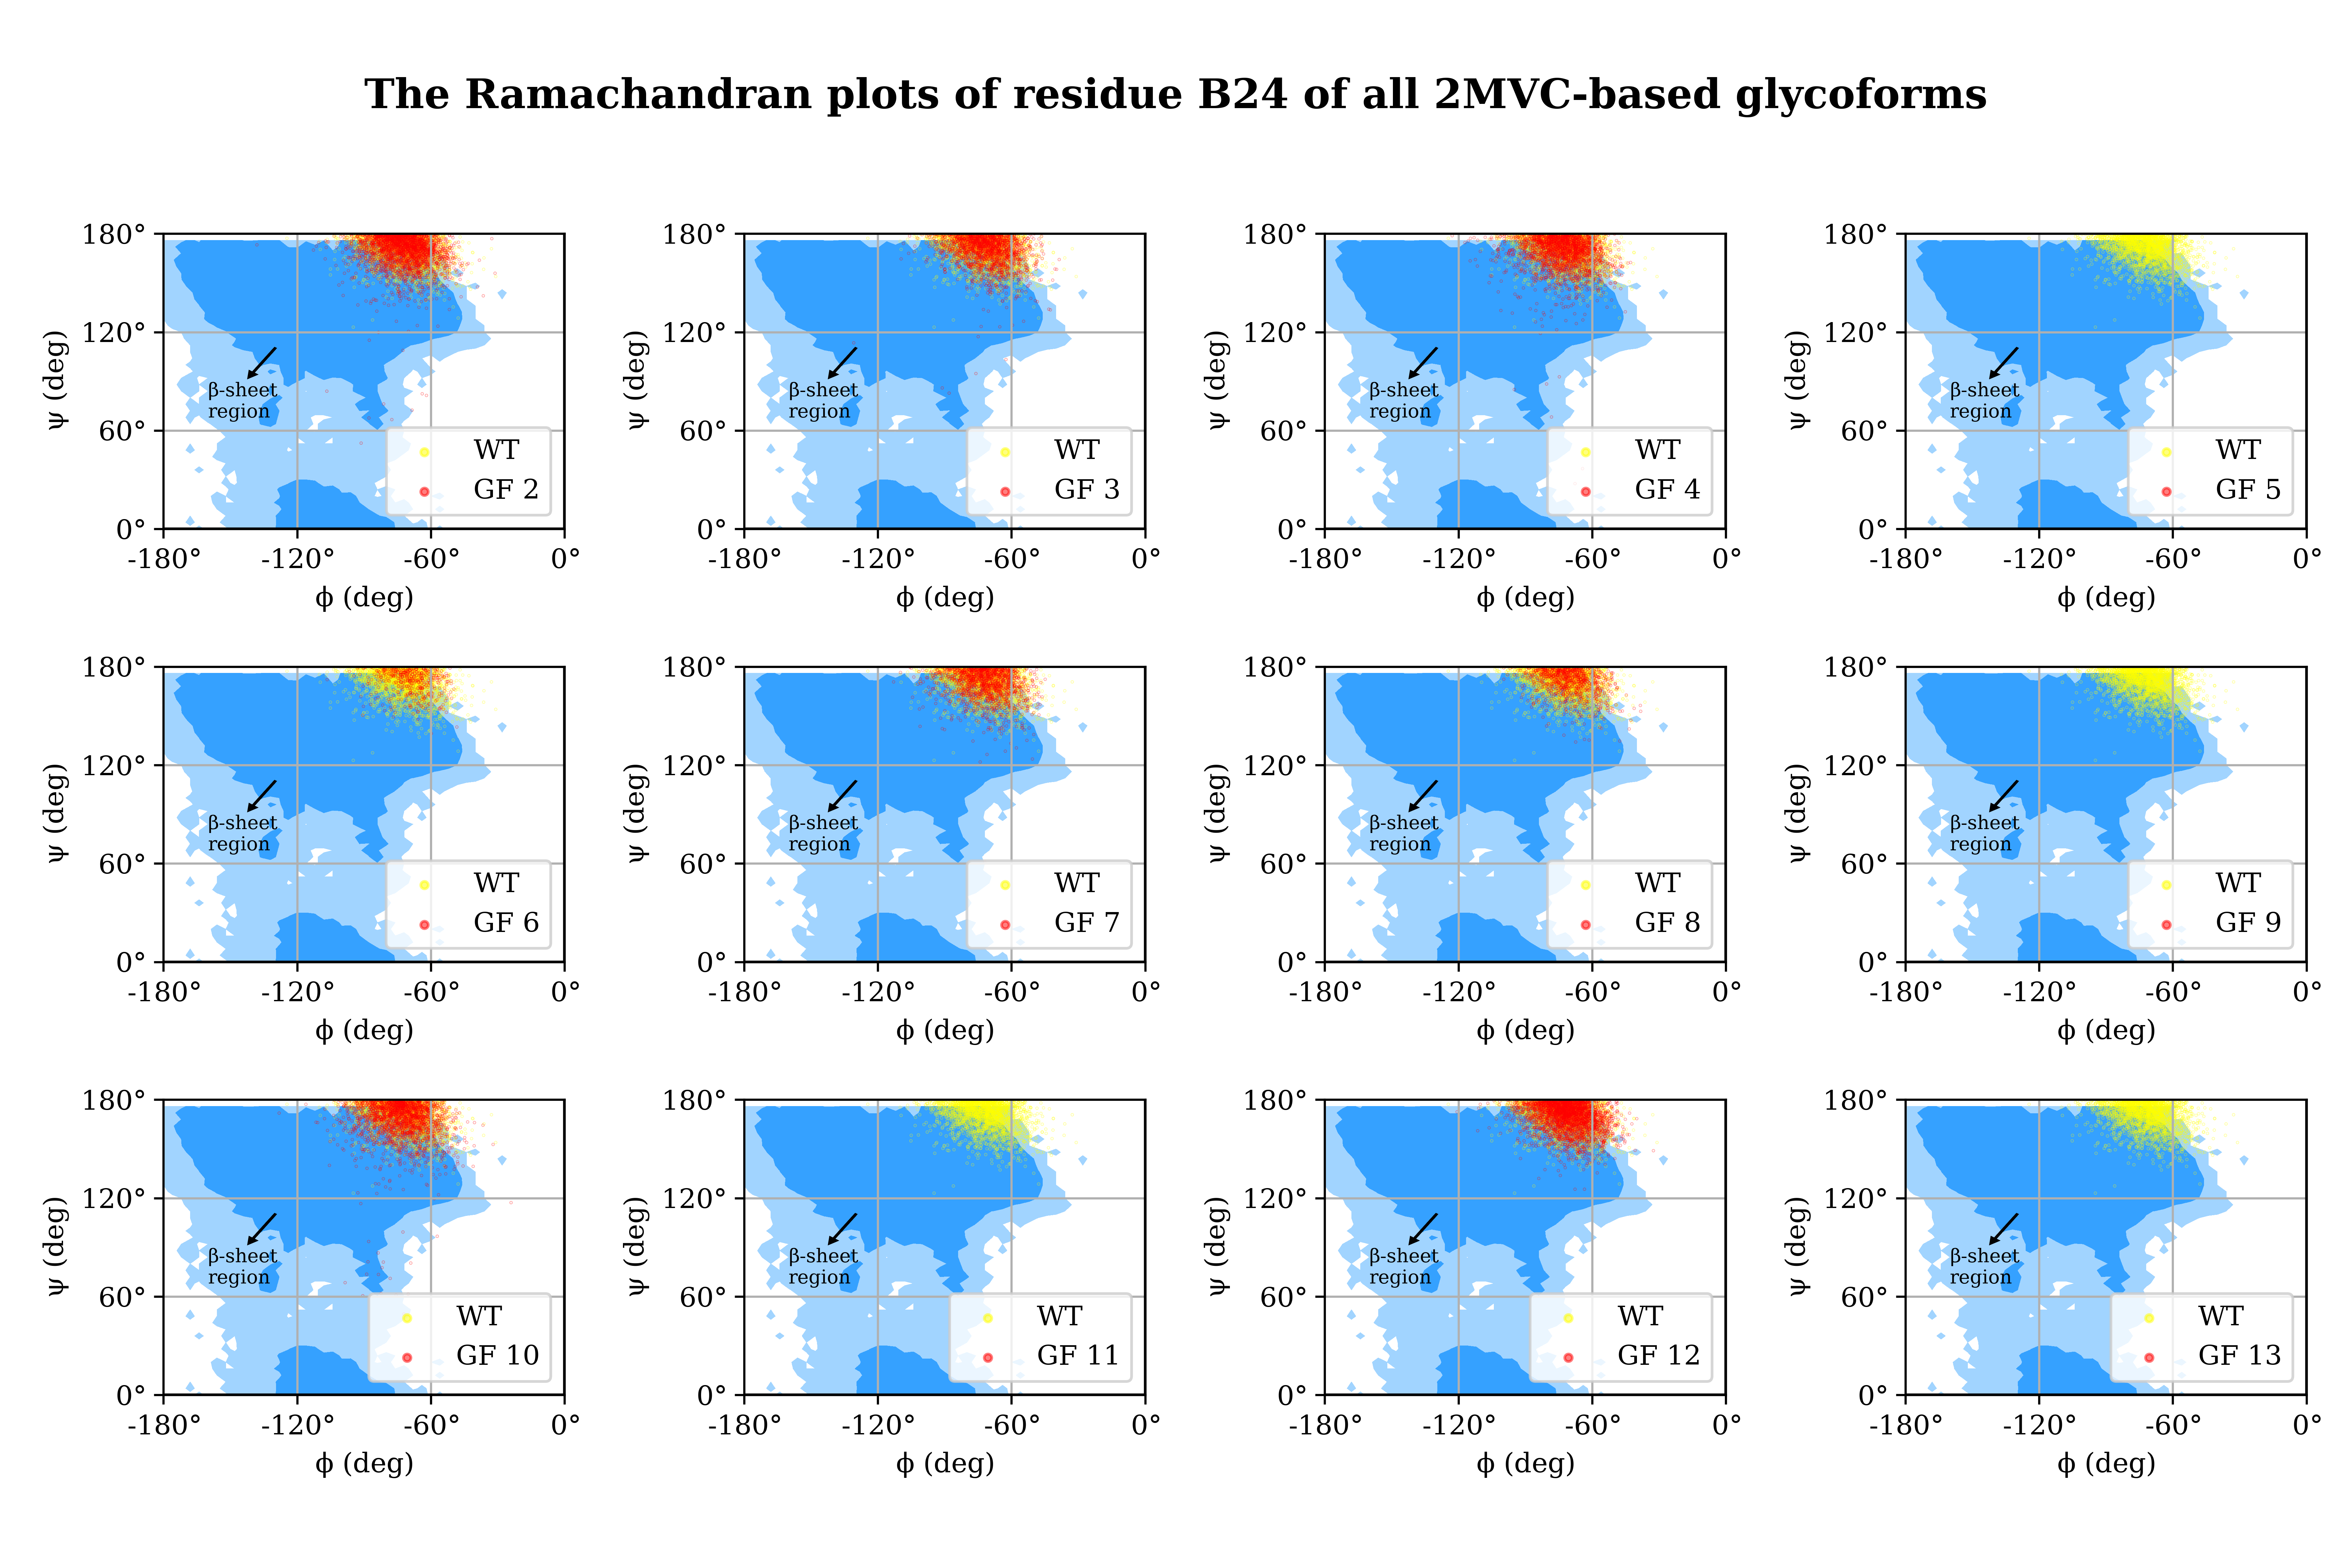
\includegraphics[width=\textwidth]{Figures/2MVC_multi_rama_plot_res_45.png}
\caption{The Ramachandran plots of residue B24 of all 2MVC-based glycoforms. The contours in the background show the allowed region in the second quadrant where the dihedral angles can reside. The deeper blue region is the $\beta$-sheet region defined by Lovell et al~\cite{lovell2003structure}.}
\end{figure}

\renewcommand{\thefigure}{S\arabic{figure}}
\begin{figure}[H]
\centering
\includegraphics[width=\textwidth]{Figures/2MVC_multi_rama_plot_res_46.png}
\caption{The Ramachandran plots of residue B25 of all 2MVC-based glycoforms. The contours in the background show the allowed region in the second quadrant where the dihedral angles can reside. The deeper blue region is the $\beta$-sheet region defined by Lovell et al~\cite{lovell2003structure}.}
\end{figure}

\renewcommand{\thefigure}{S\arabic{figure}}
\begin{figure}[H]
\centering
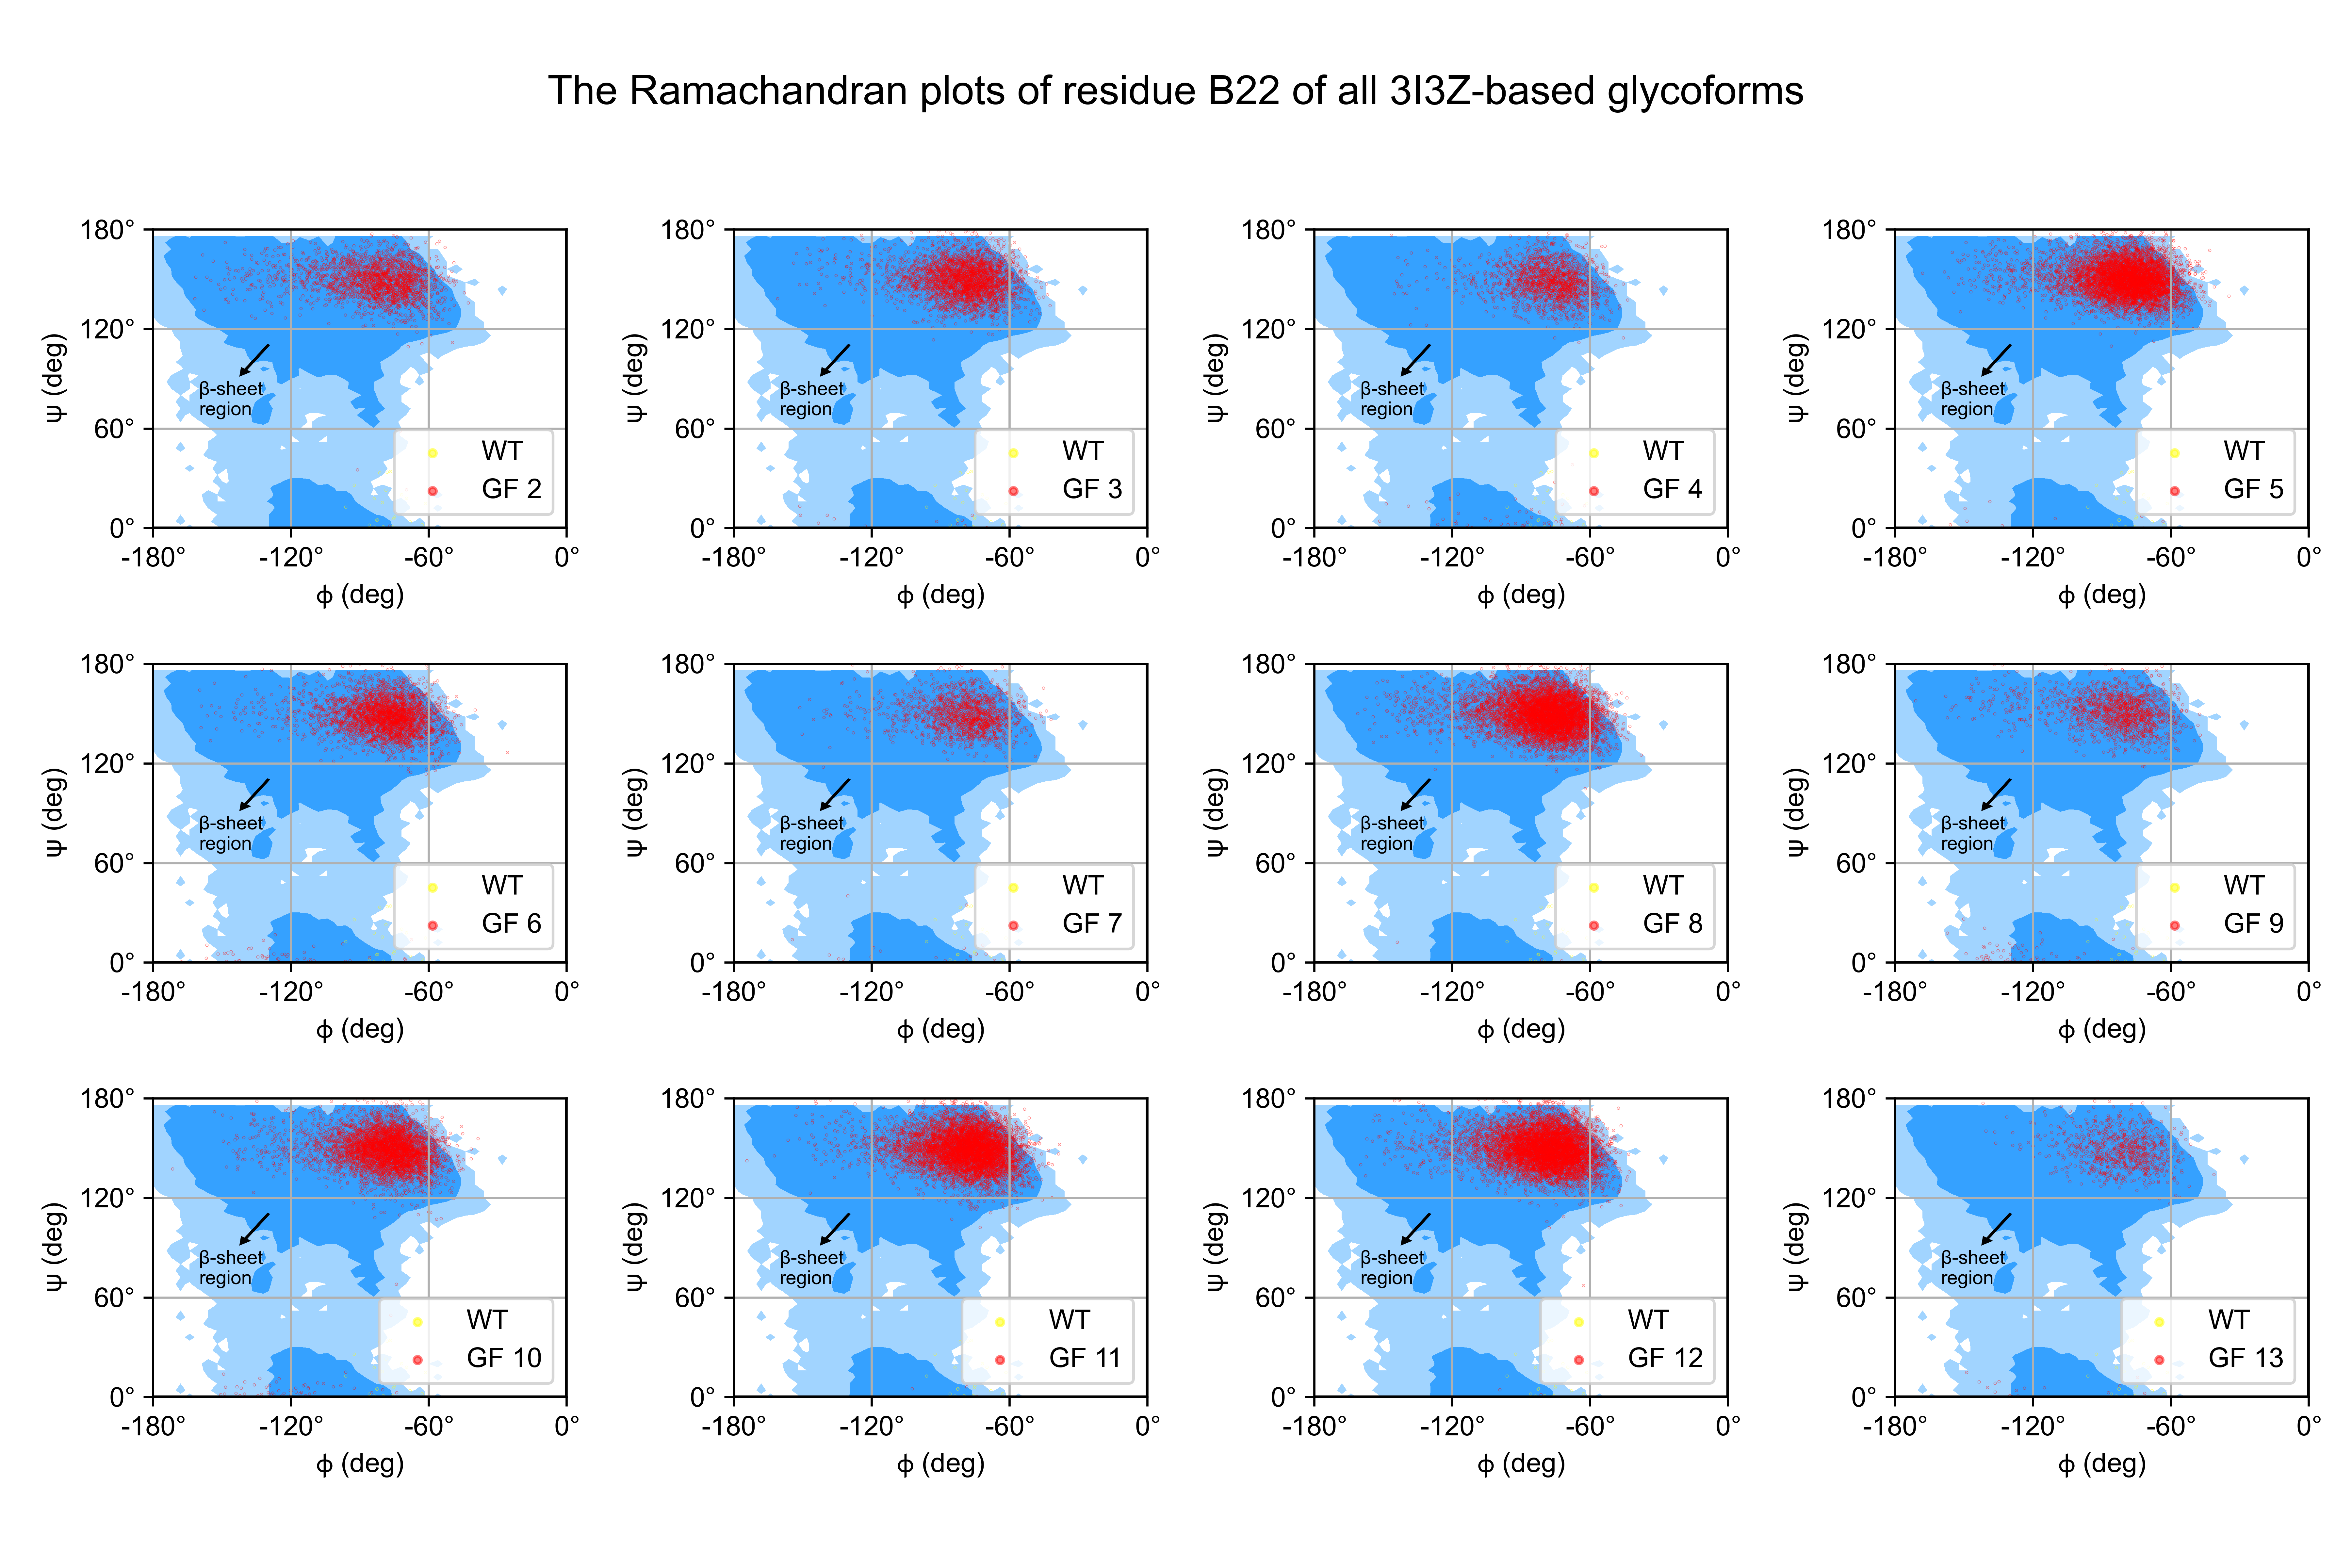
\includegraphics[width=\textwidth]{Figures/3I3Z_multi_rama_plot_res_43.png}
\caption{The Ramachandran plots of residue B22 of all 3I3Z-based glycoforms. The contours in the background show the allowed region in the second quadrant where the dihedral angles can reside. The deeper blue region is the $\beta$-sheet region defined by Lovell et al~\cite{lovell2003structure}.}
\end{figure}

\renewcommand{\thefigure}{S\arabic{figure}}
\begin{figure}[H]
\centering
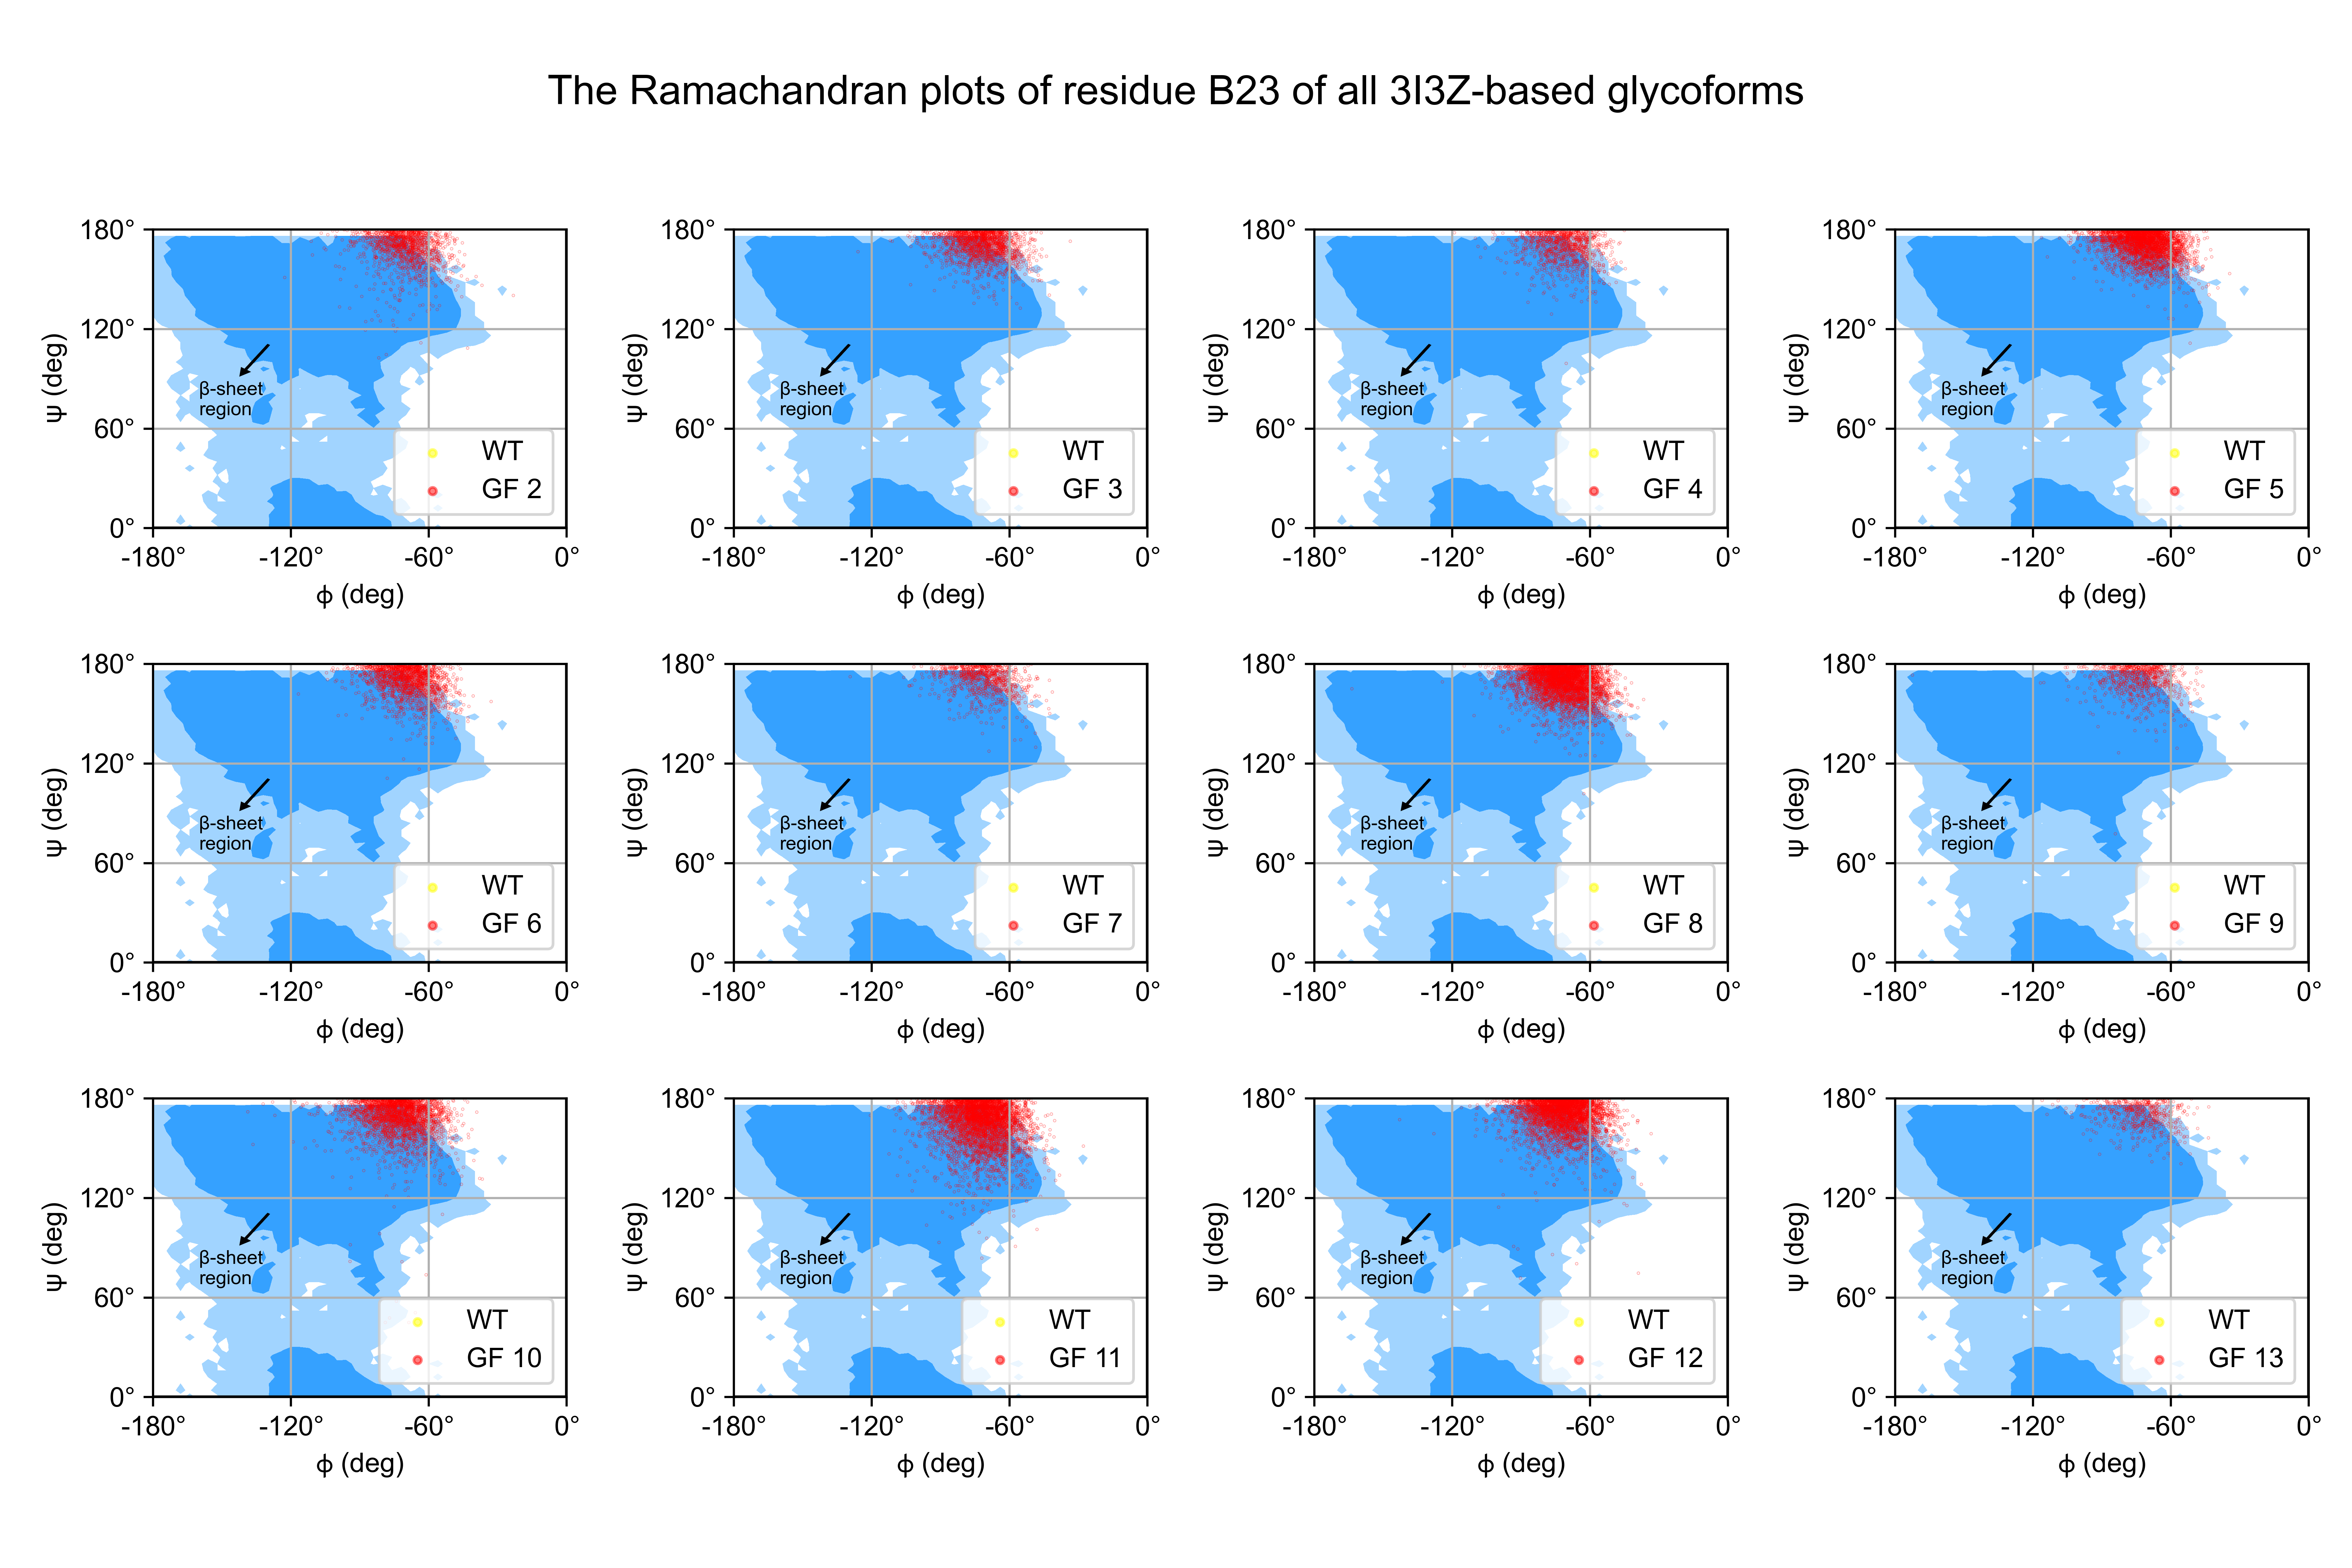
\includegraphics[width=\textwidth]{Figures/3I3Z_multi_rama_plot_res_44.png}
\caption{The Ramachandran plots of residue B23 of all 3I3Z-based glycoforms. The contours in the background show the allowed region in the second quadrant where the dihedral angles can reside. The deeper blue region is the $\beta$-sheet region defined by Lovell et al~\cite{lovell2003structure}.}
\end{figure}

\renewcommand{\thefigure}{S\arabic{figure}}
\begin{figure}[H]
\centering
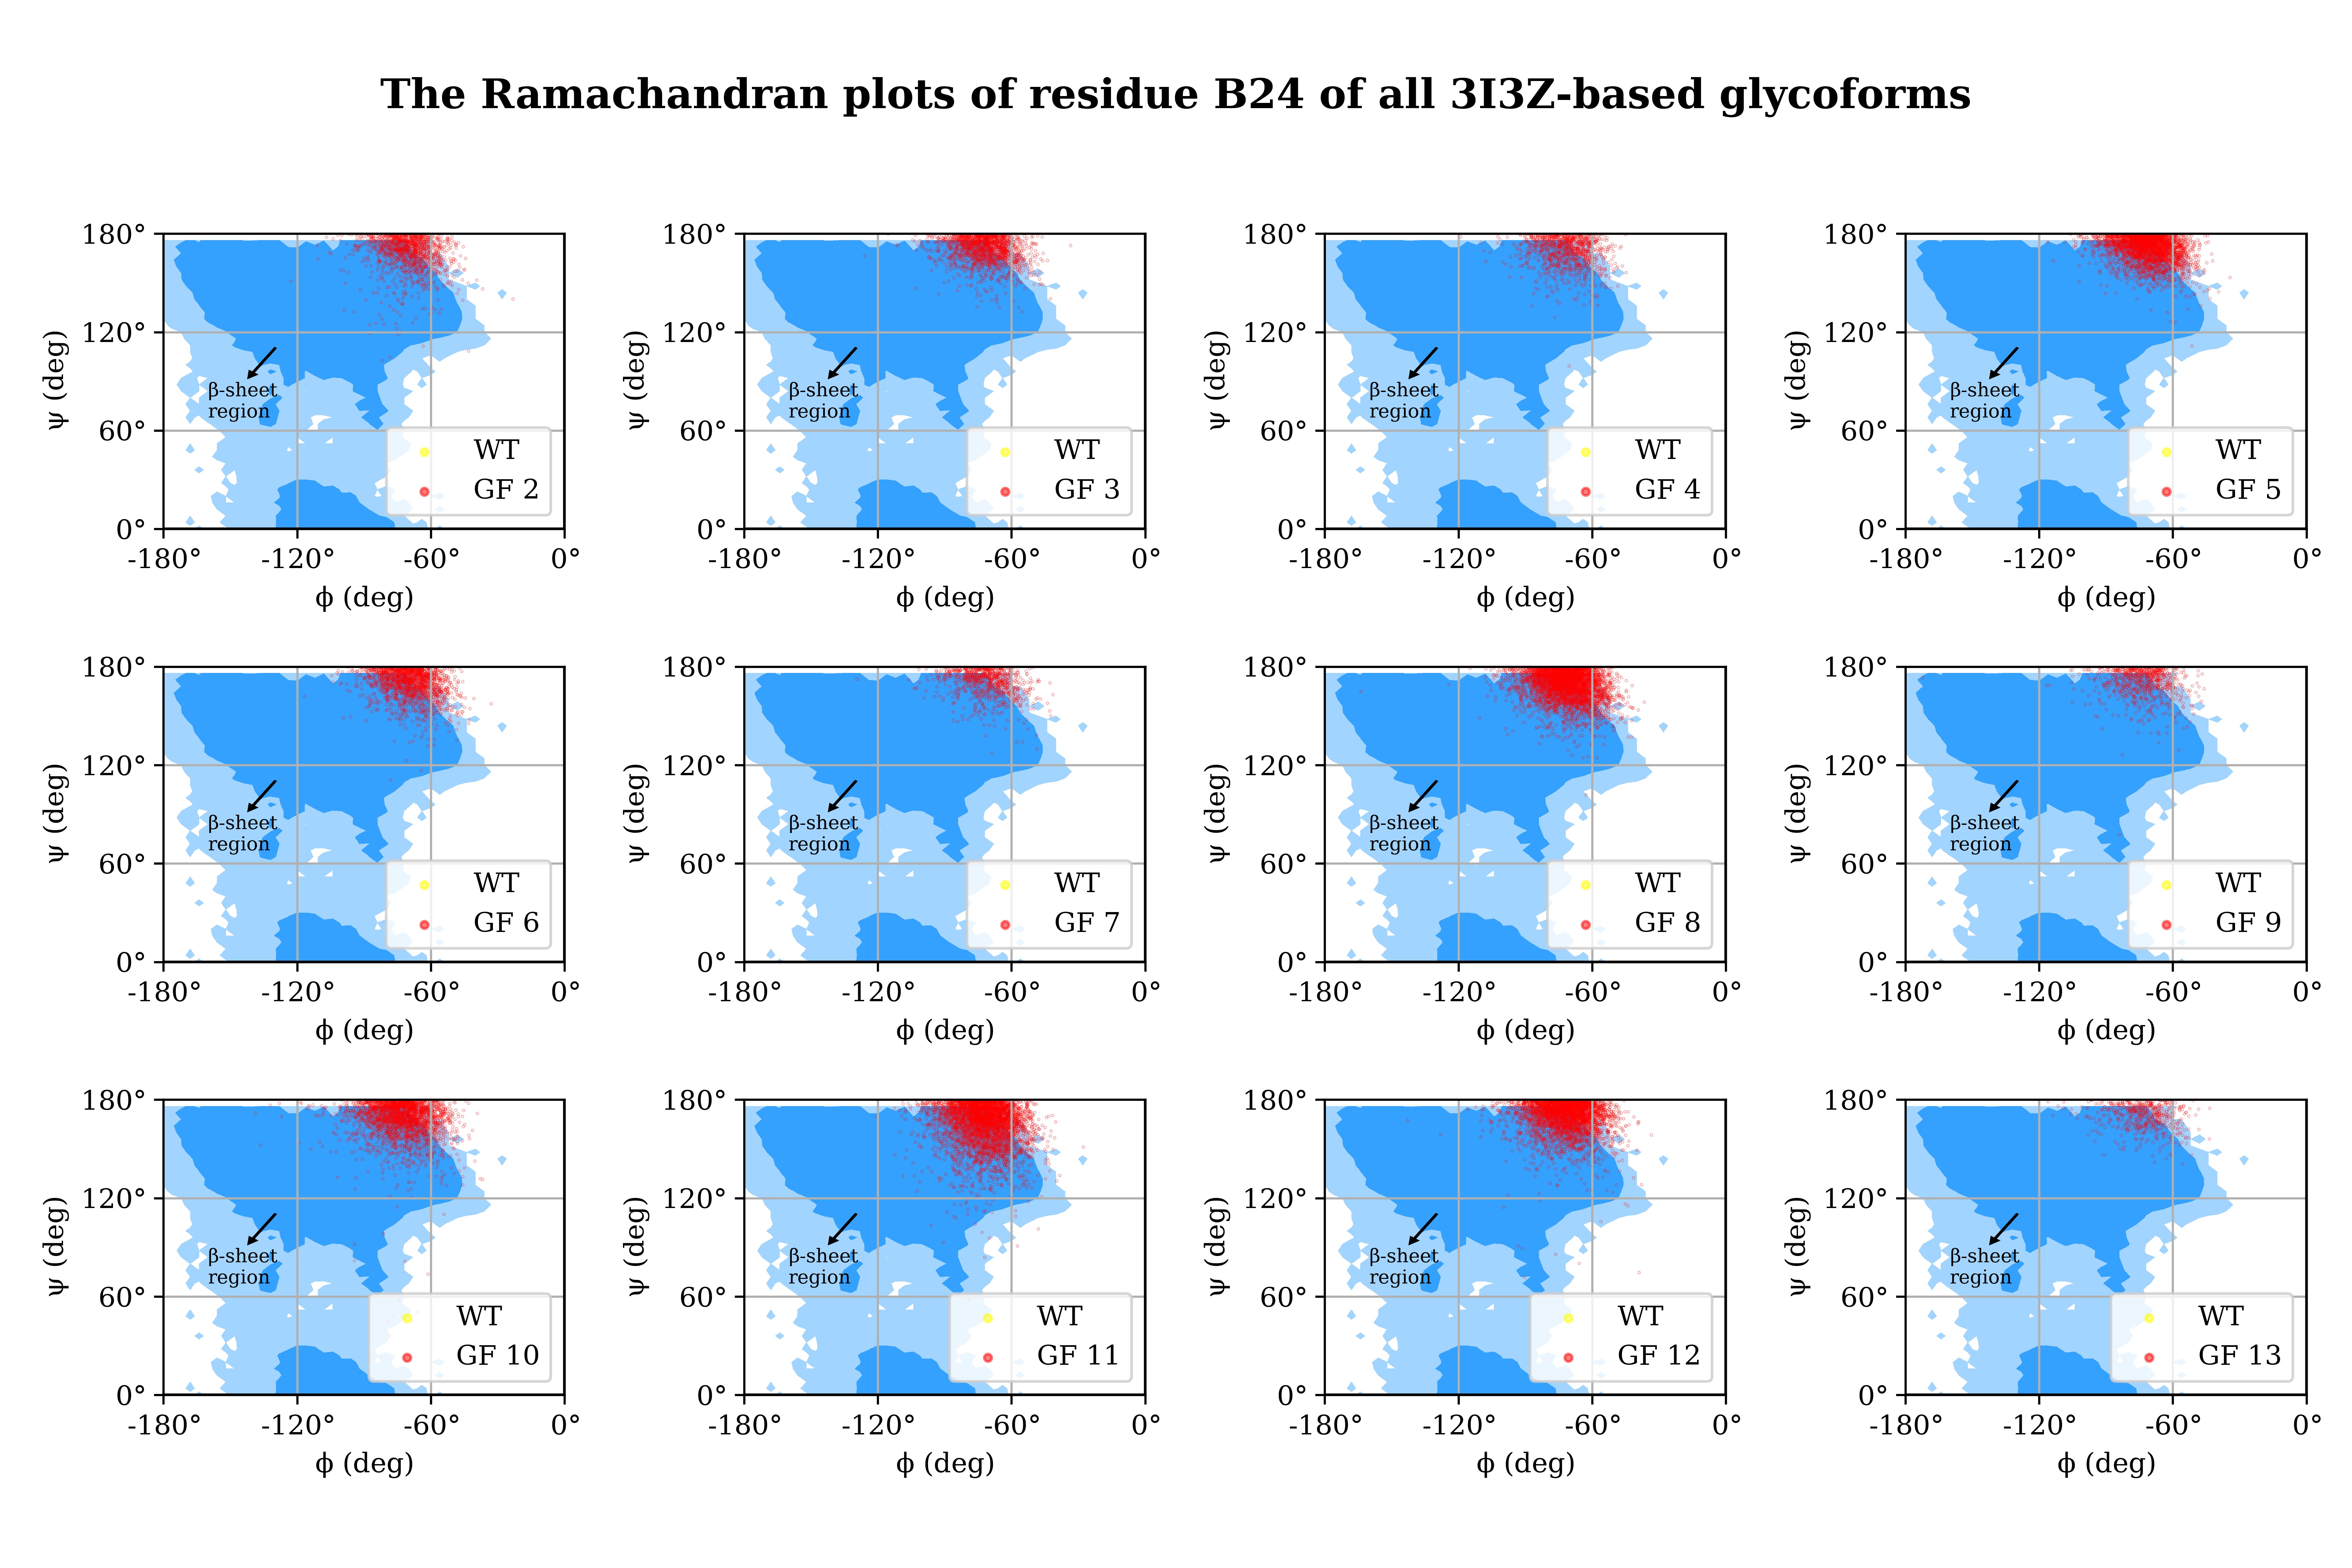
\includegraphics[width=\textwidth]{Figures/3I3Z_multi_rama_plot_res_45.png}
\caption{The Ramachandran plots of residue B24 of all 3I3Z-based glycoforms. The contours in the background show the allowed region in the second quadrant where the dihedral angles can reside. The deeper blue region is the $\beta$-sheet region defined by Lovell et al~\cite{lovell2003structure}.}
\end{figure}

\renewcommand{\thefigure}{S\arabic{figure}}
\begin{figure}[H]
\centering
\includegraphics[width=\textwidth]{Figures/3I3Z_multi_rama_plot_res_46.png}
\caption{The Ramachandran plots of residue B25 of all 3I3Z-based glycoforms. The contours in the background show the allowed region in the second quadrant where the dihedral angles can reside. The deeper blue region is the $\beta$-sheet region defined by Lovell et al~\cite{lovell2003structure}.}
\end{figure}

\renewcommand{\thefigure}{S\arabic{figure}}
\begin{figure}[H]
\centering
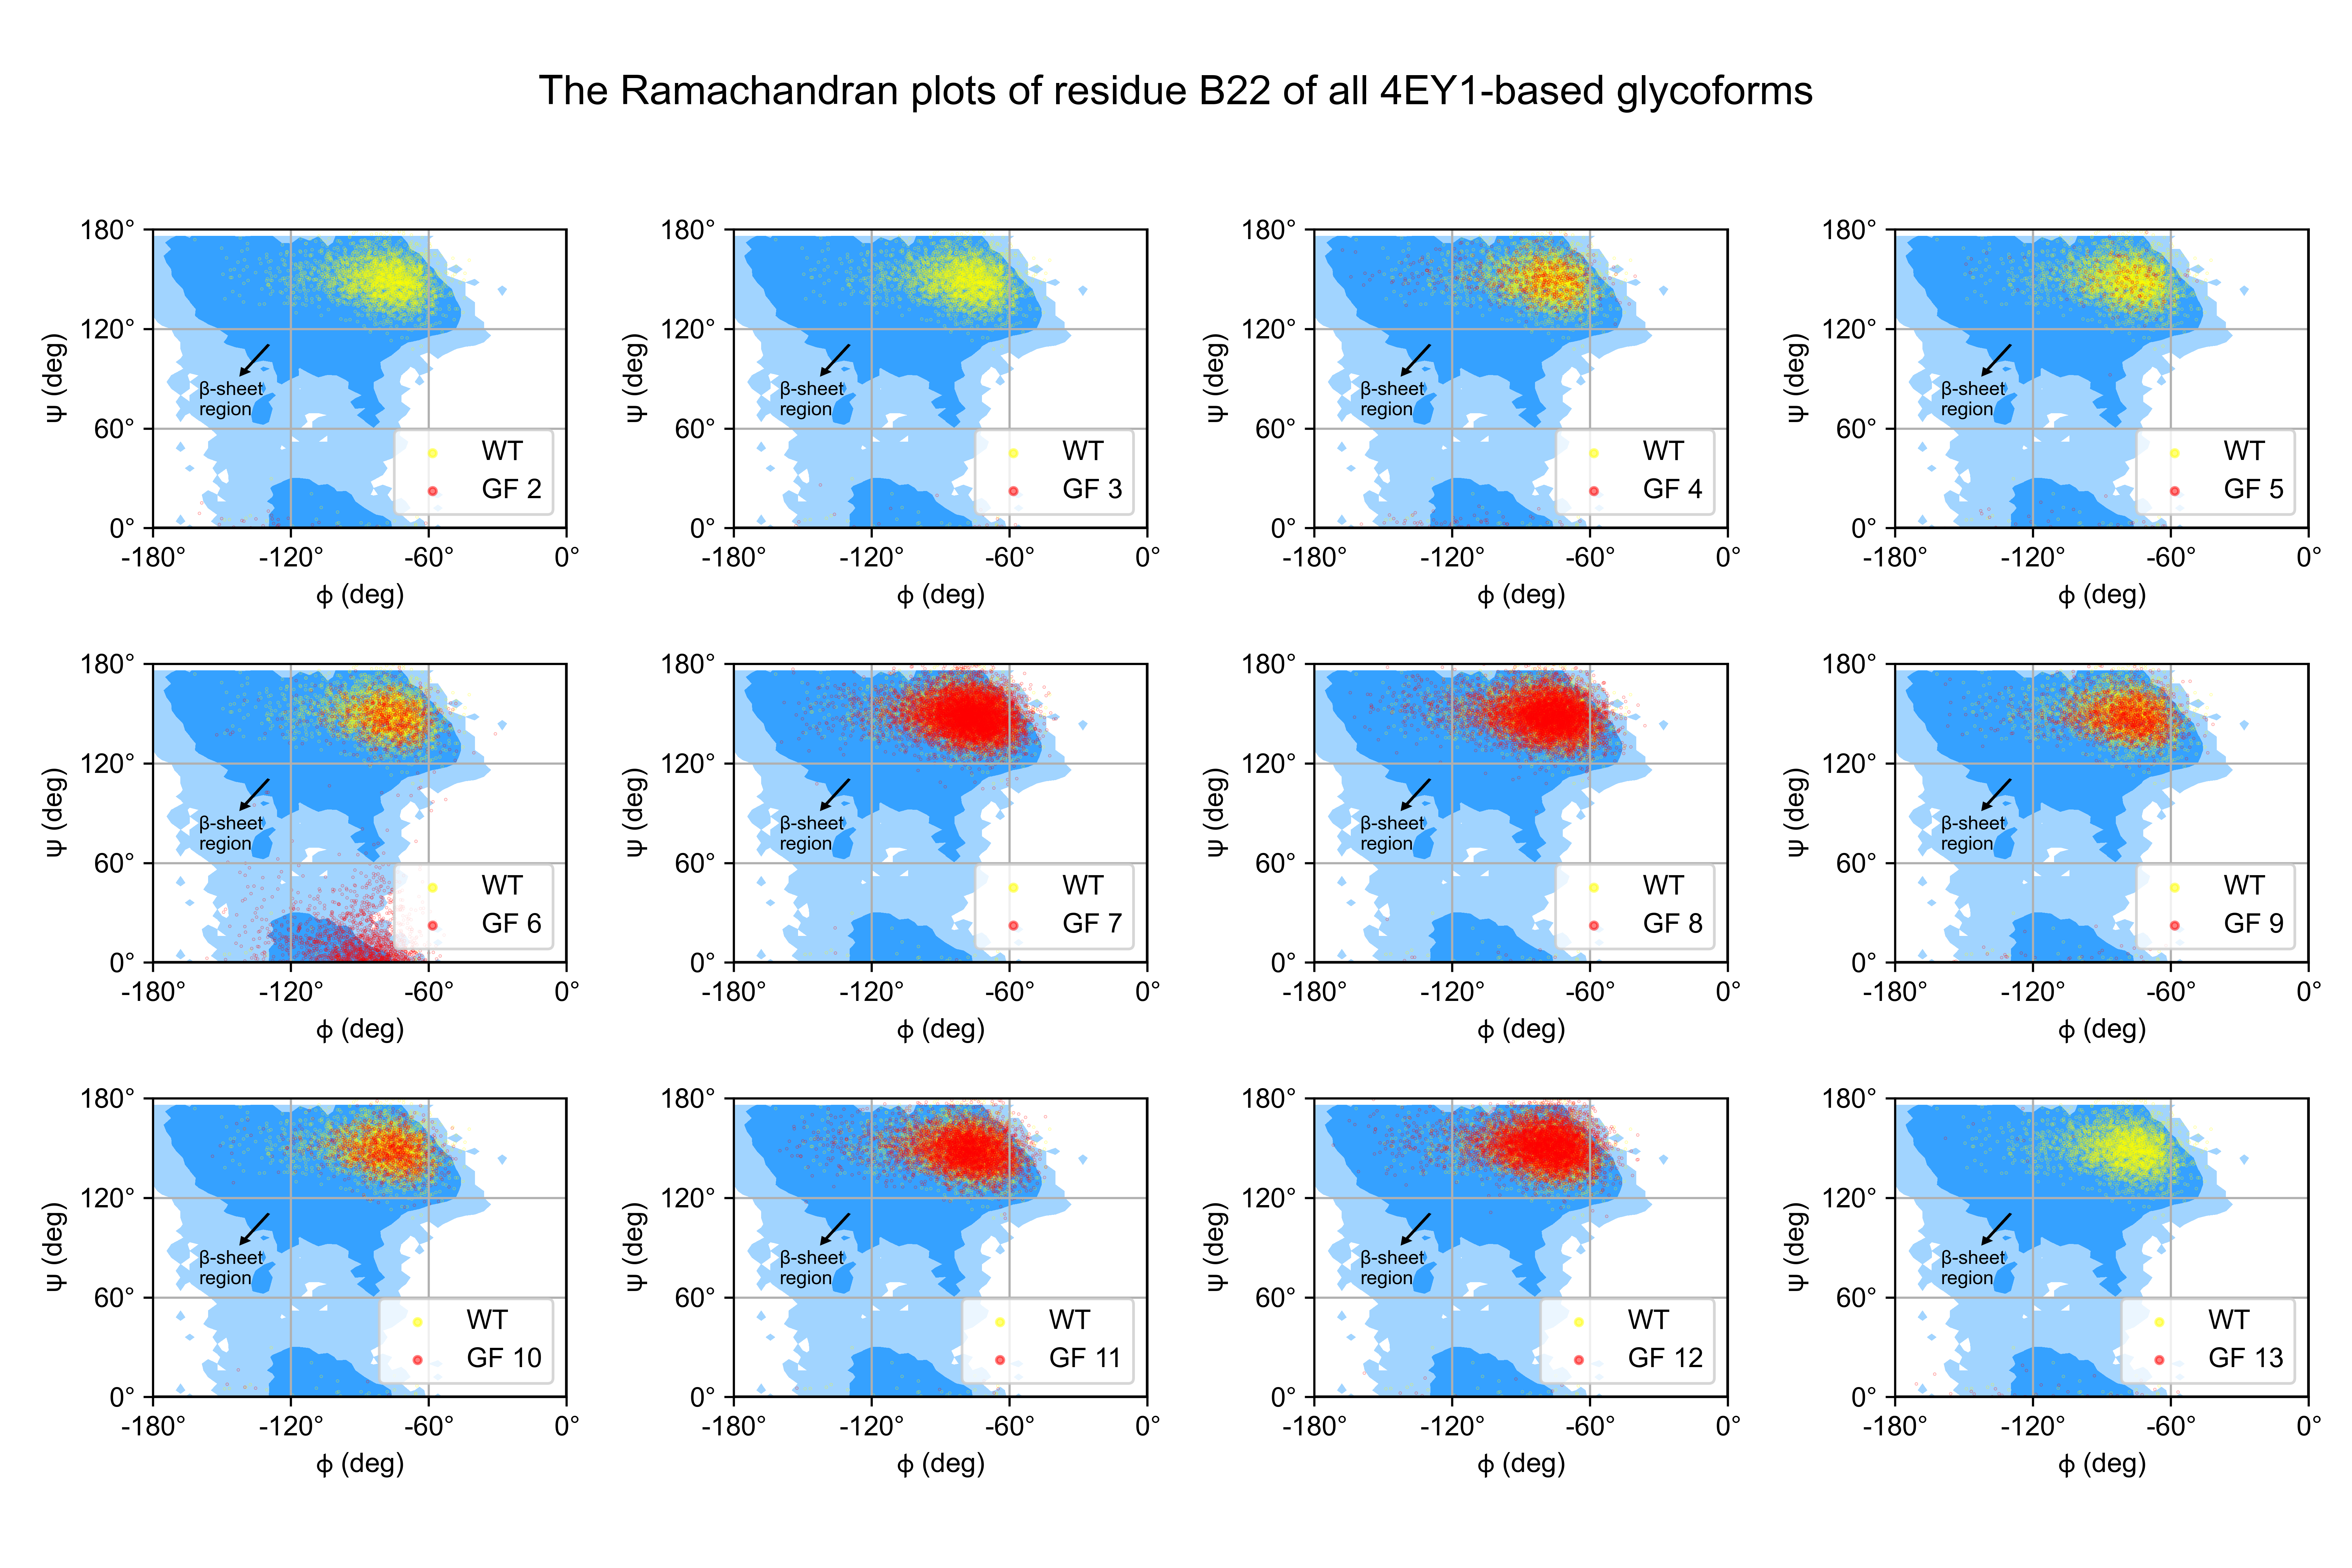
\includegraphics[width=\textwidth]{Figures/4EY1_multi_rama_plot_res_43.png}
\caption{The Ramachandran plots of residue B22 of all 4EY1-based glycoforms. The contours in the background show the allowed region in the second quadrant where the dihedral angles can reside. The deeper blue region is the $\beta$-sheet region defined by Lovell et al~\cite{lovell2003structure}.}
\end{figure}

\renewcommand{\thefigure}{S\arabic{figure}}
\begin{figure}[H]
\centering
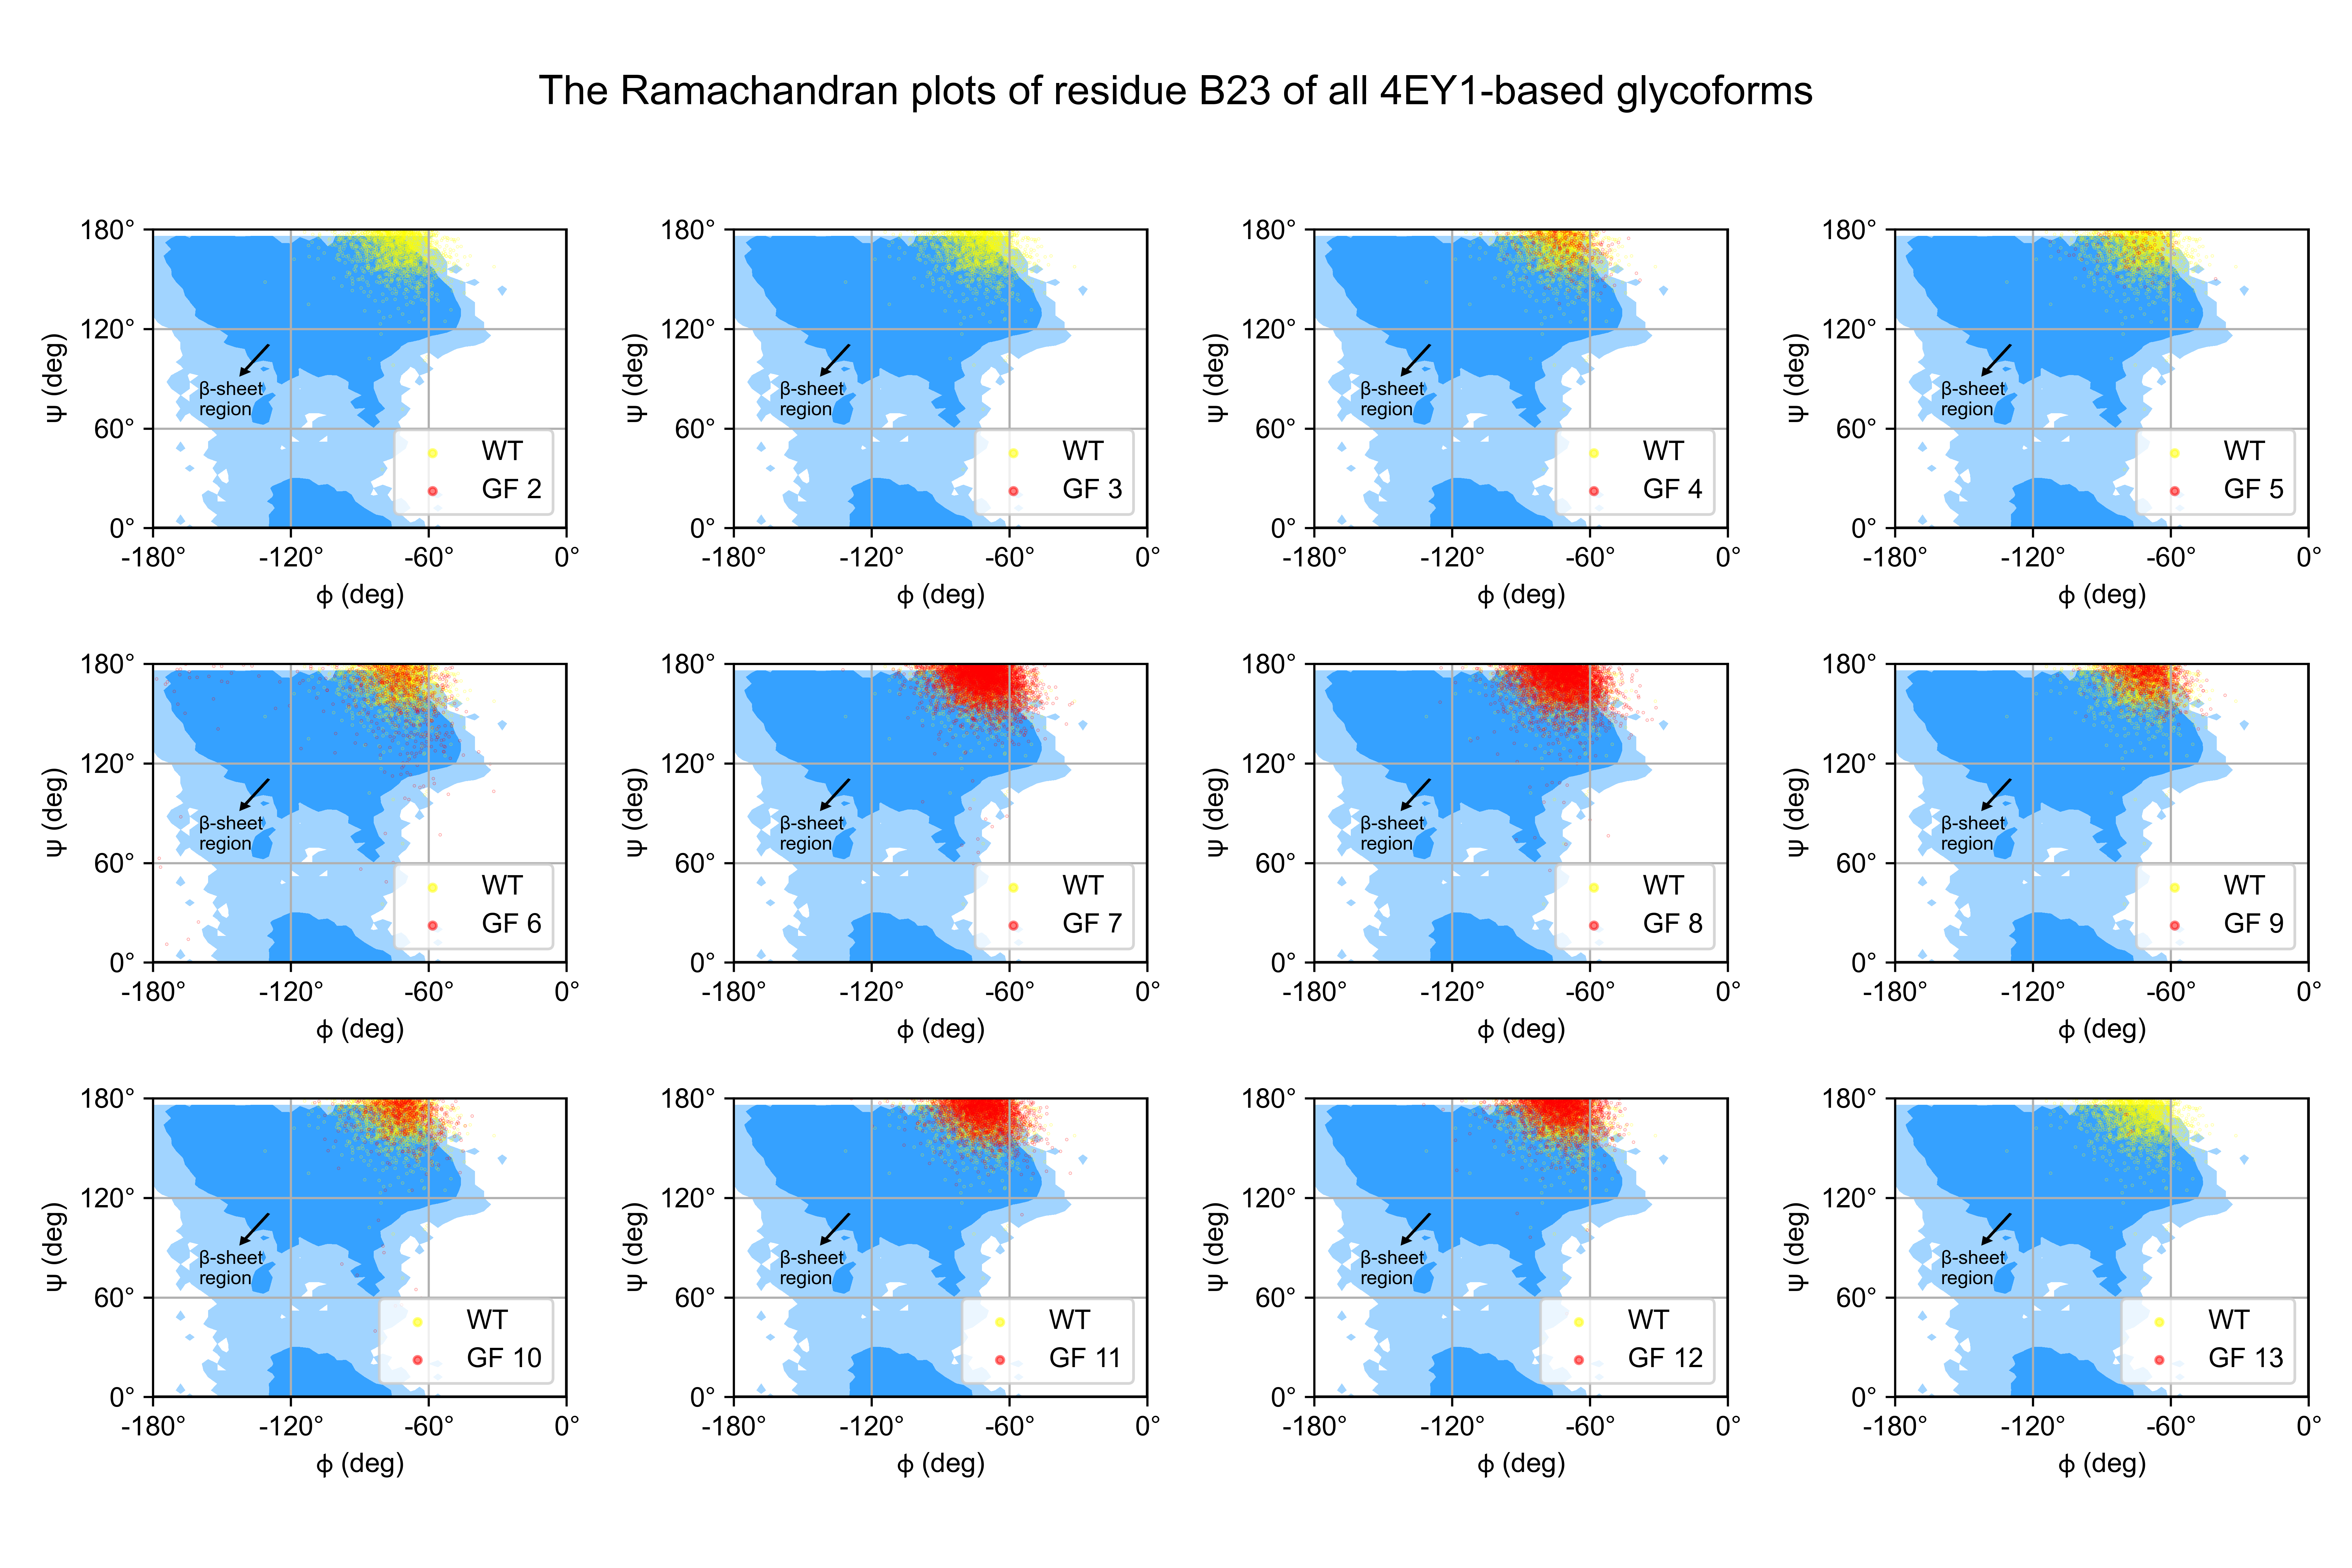
\includegraphics[width=\textwidth]{Figures/4EY1_multi_rama_plot_res_44.png}
\caption{The Ramachandran plots of residue B23 of all 4EY1-based glycoforms. The contours in the background show the allowed region in the second quadrant where the dihedral angles can reside. The deeper blue region is the $\beta$-sheet region defined by Lovell et al~\cite{lovell2003structure}.}
\end{figure}

\renewcommand{\thefigure}{S\arabic{figure}}
\begin{figure}[H]
\centering
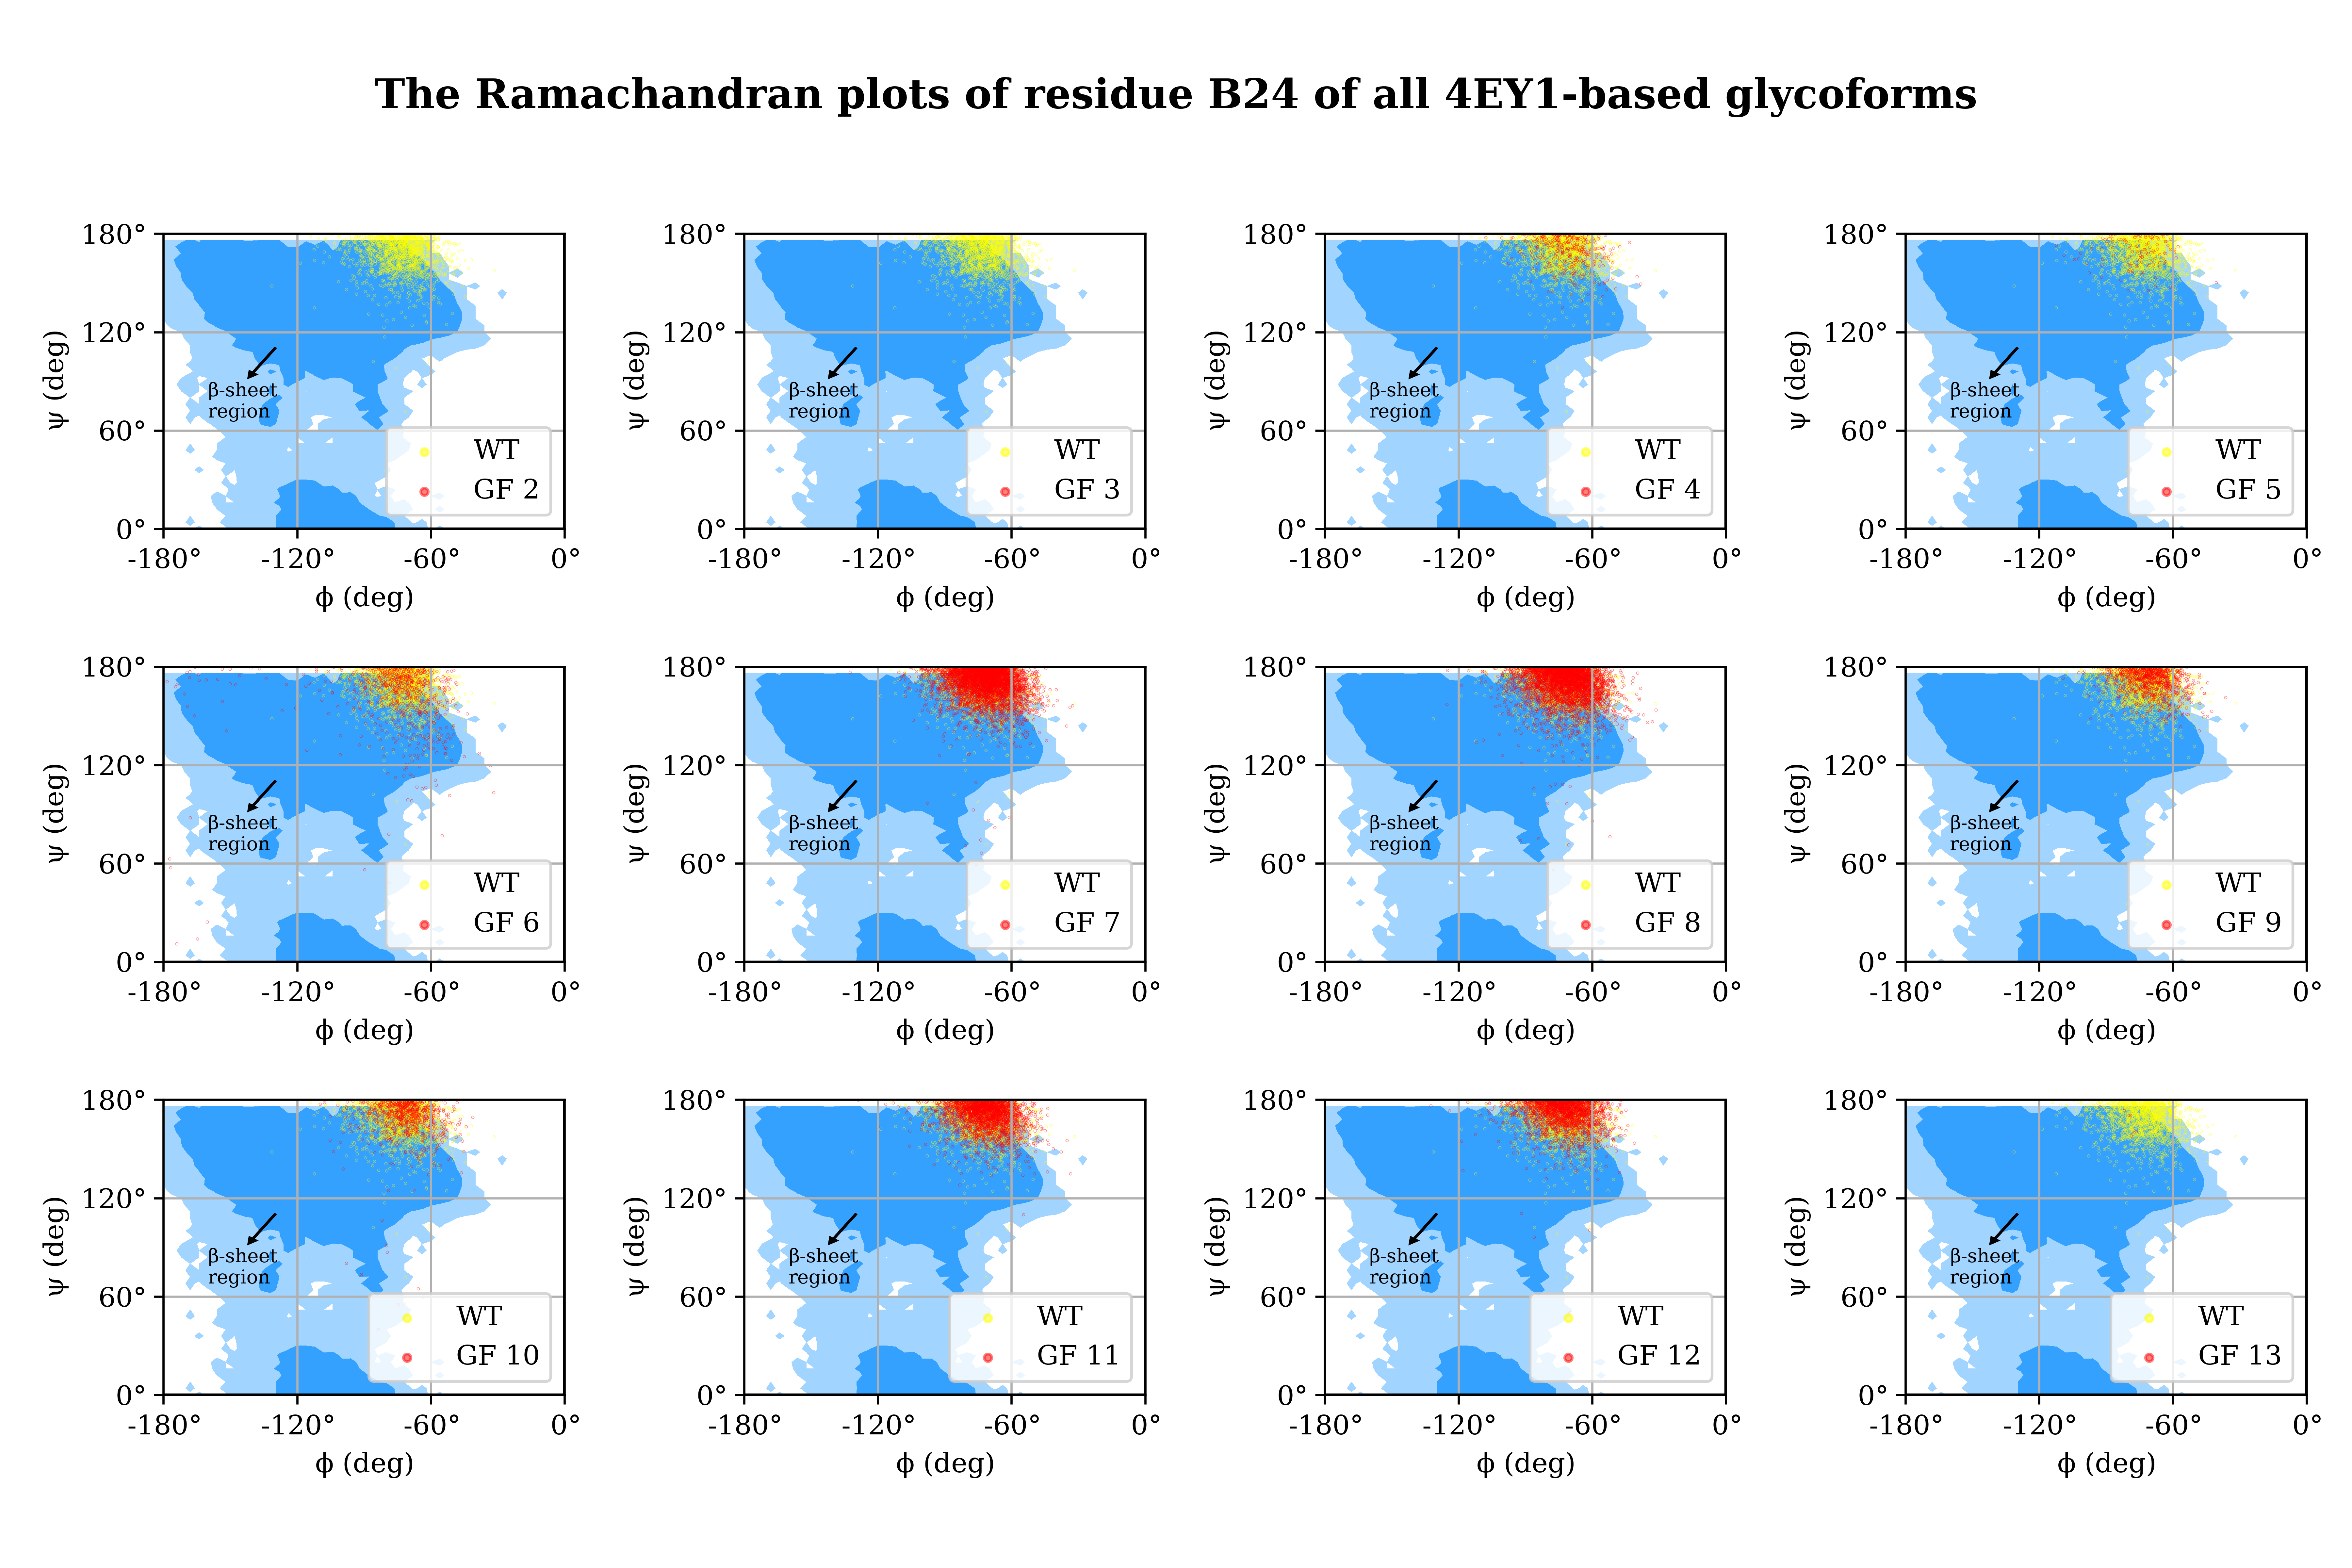
\includegraphics[width=\textwidth]{Figures/4EY1_multi_rama_plot_res_45.png}
\caption{The Ramachandran plots of residue B24 of all 4EY1-based glycoforms. The contours in the background show the allowed region in the second quadrant where the dihedral angles can reside. The deeper blue region is the $\beta$-sheet region defined by Lovell et al~\cite{lovell2003structure}.}
\end{figure}

\renewcommand{\thefigure}{S\arabic{figure}}
\begin{figure}[H]
\centering
\includegraphics[width=\textwidth]{Figures/4EY1_multi_rama_plot_res_46.png}
\caption{The Ramachandran plots of residue B25 of all 4EY1-based glycoforms. The contours in the background show the allowed region in the second quadrant where the dihedral angles can reside. The deeper blue region is the $\beta$-sheet region defined by Lovell et al~\cite{lovell2003structure}.}
\end{figure}

\renewcommand{\thefigure}{S\arabic{figure}}
\begin{figure}[H]
\centering
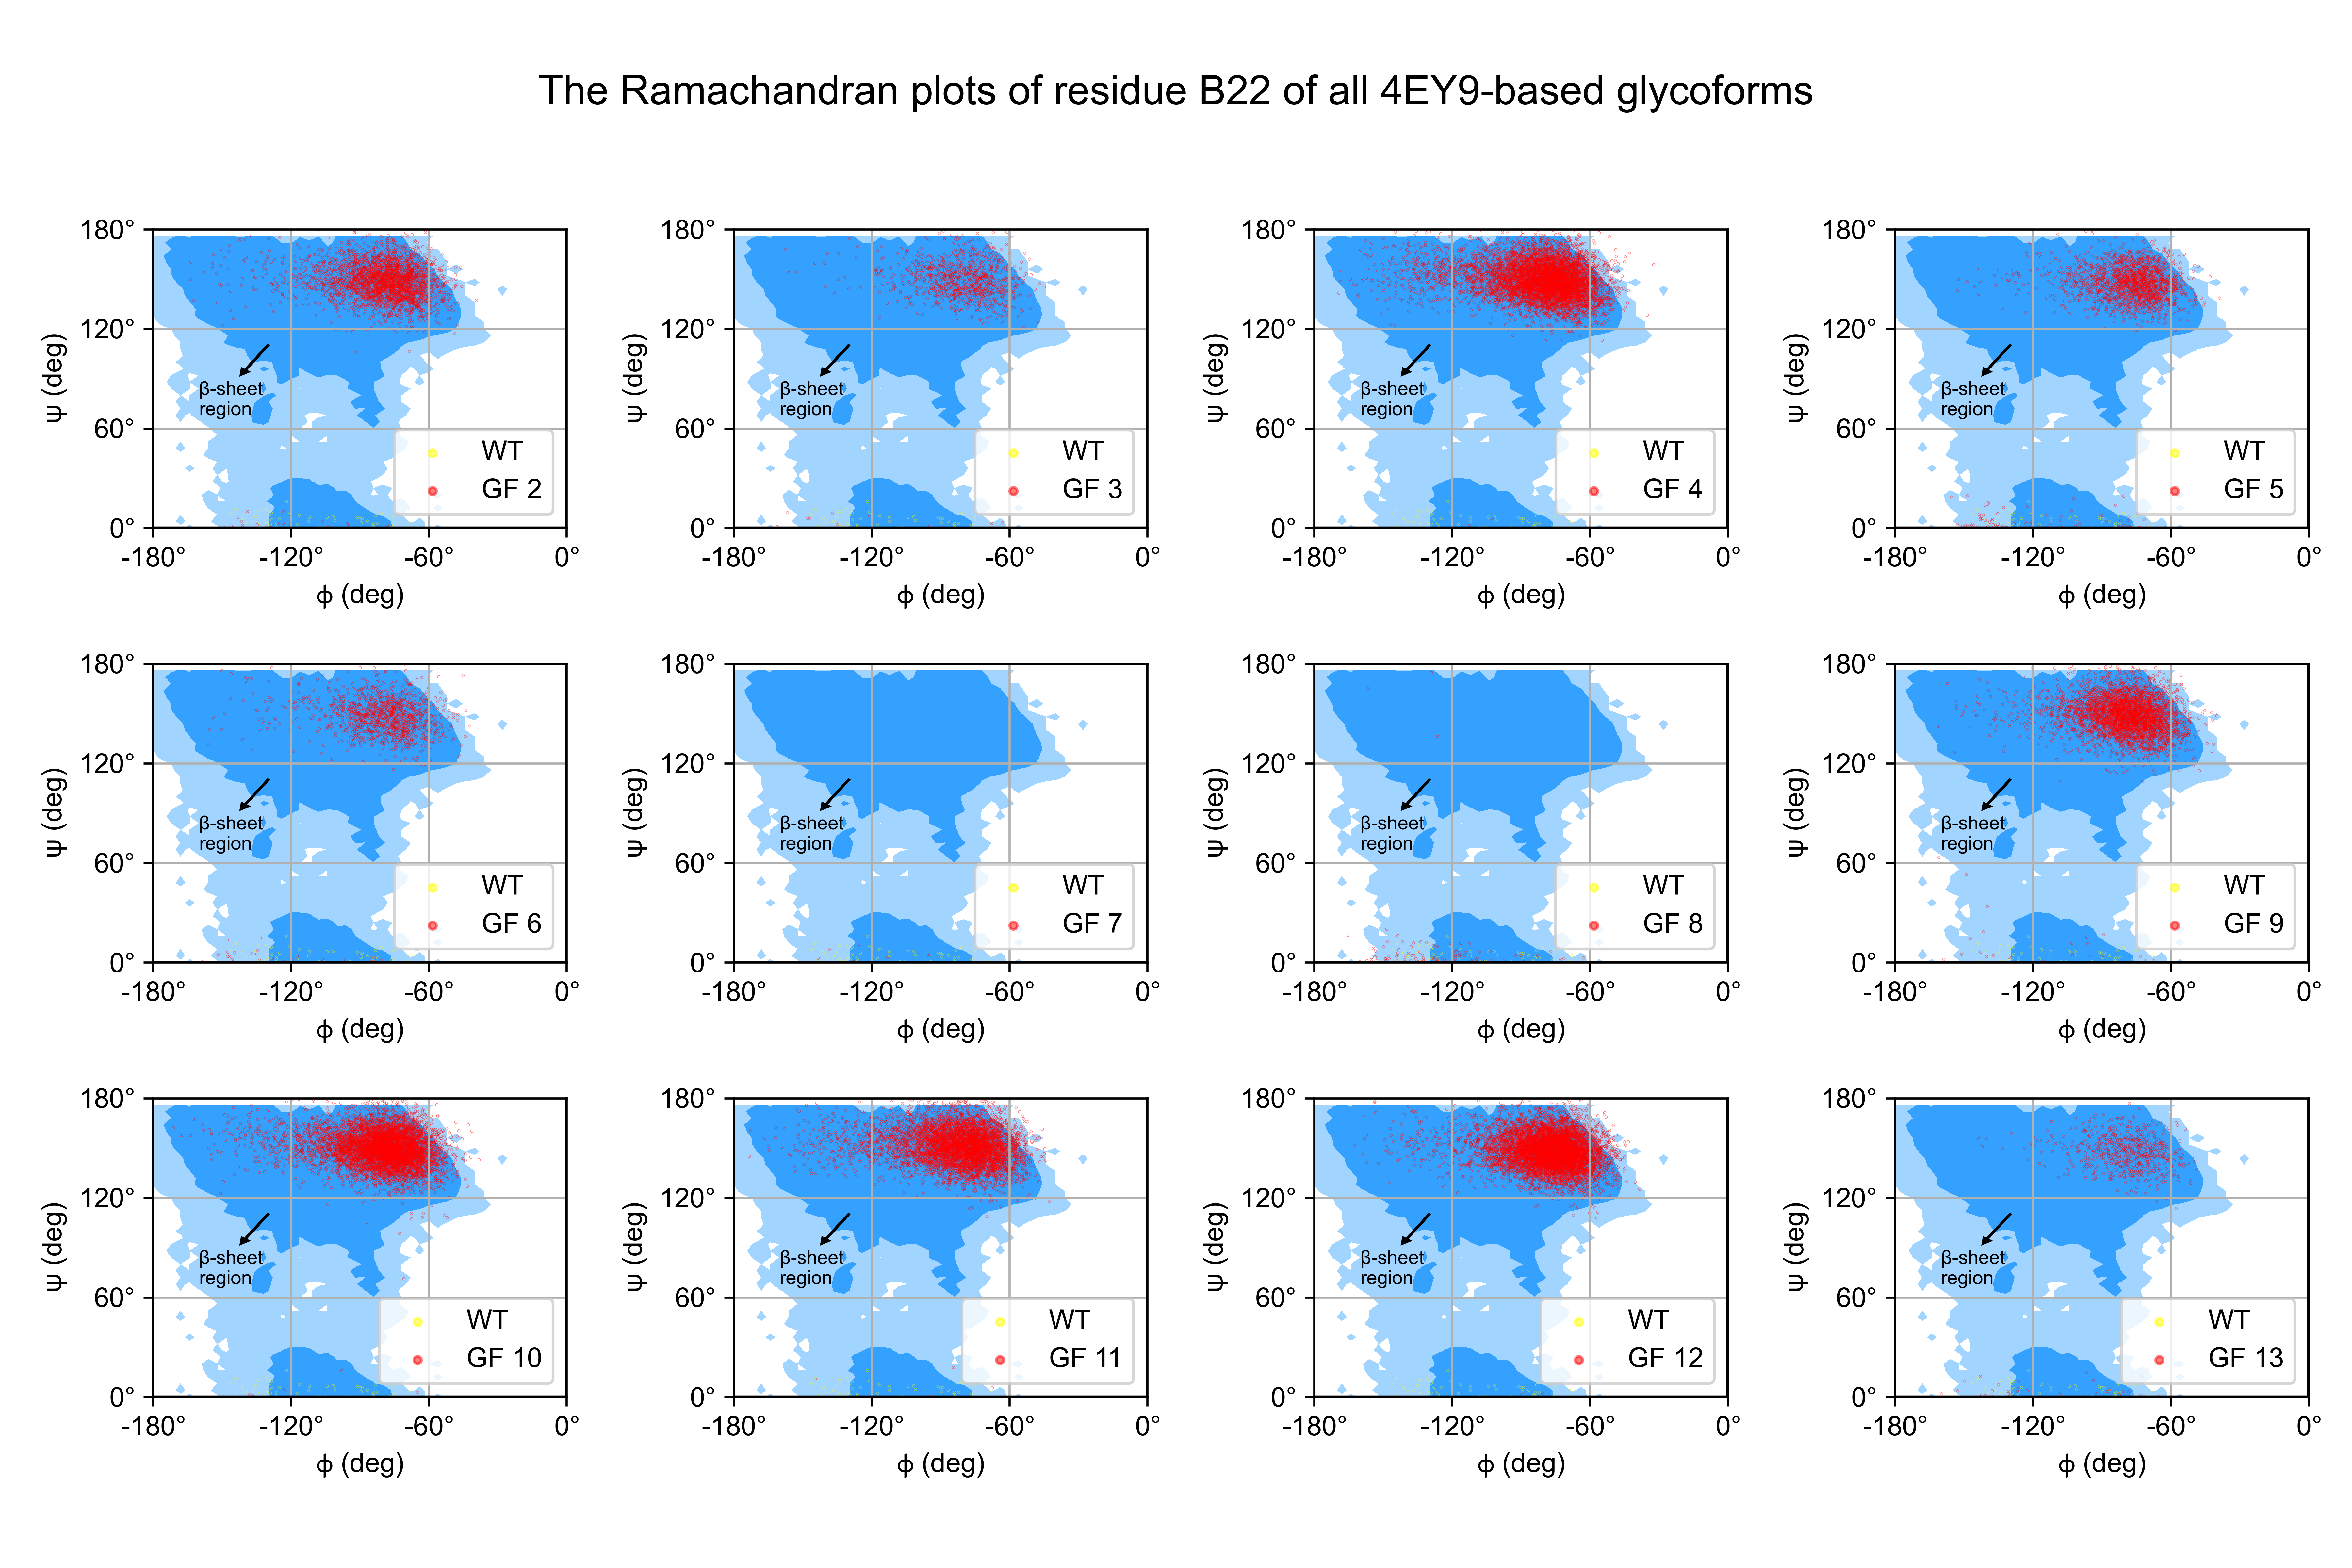
\includegraphics[width=\textwidth]{Figures/4EY9_multi_rama_plot_res_43.png}
\caption{The Ramachandran plots of residue B22 of all 4EY9-based glycoforms. The contours in the background show the allowed region in the second quadrant where the dihedral angles can reside. The deeper blue region is the $\beta$-sheet region defined by Lovell et al~\cite{lovell2003structure}.}
\end{figure}

\renewcommand{\thefigure}{S\arabic{figure}}
\begin{figure}[H]
\centering
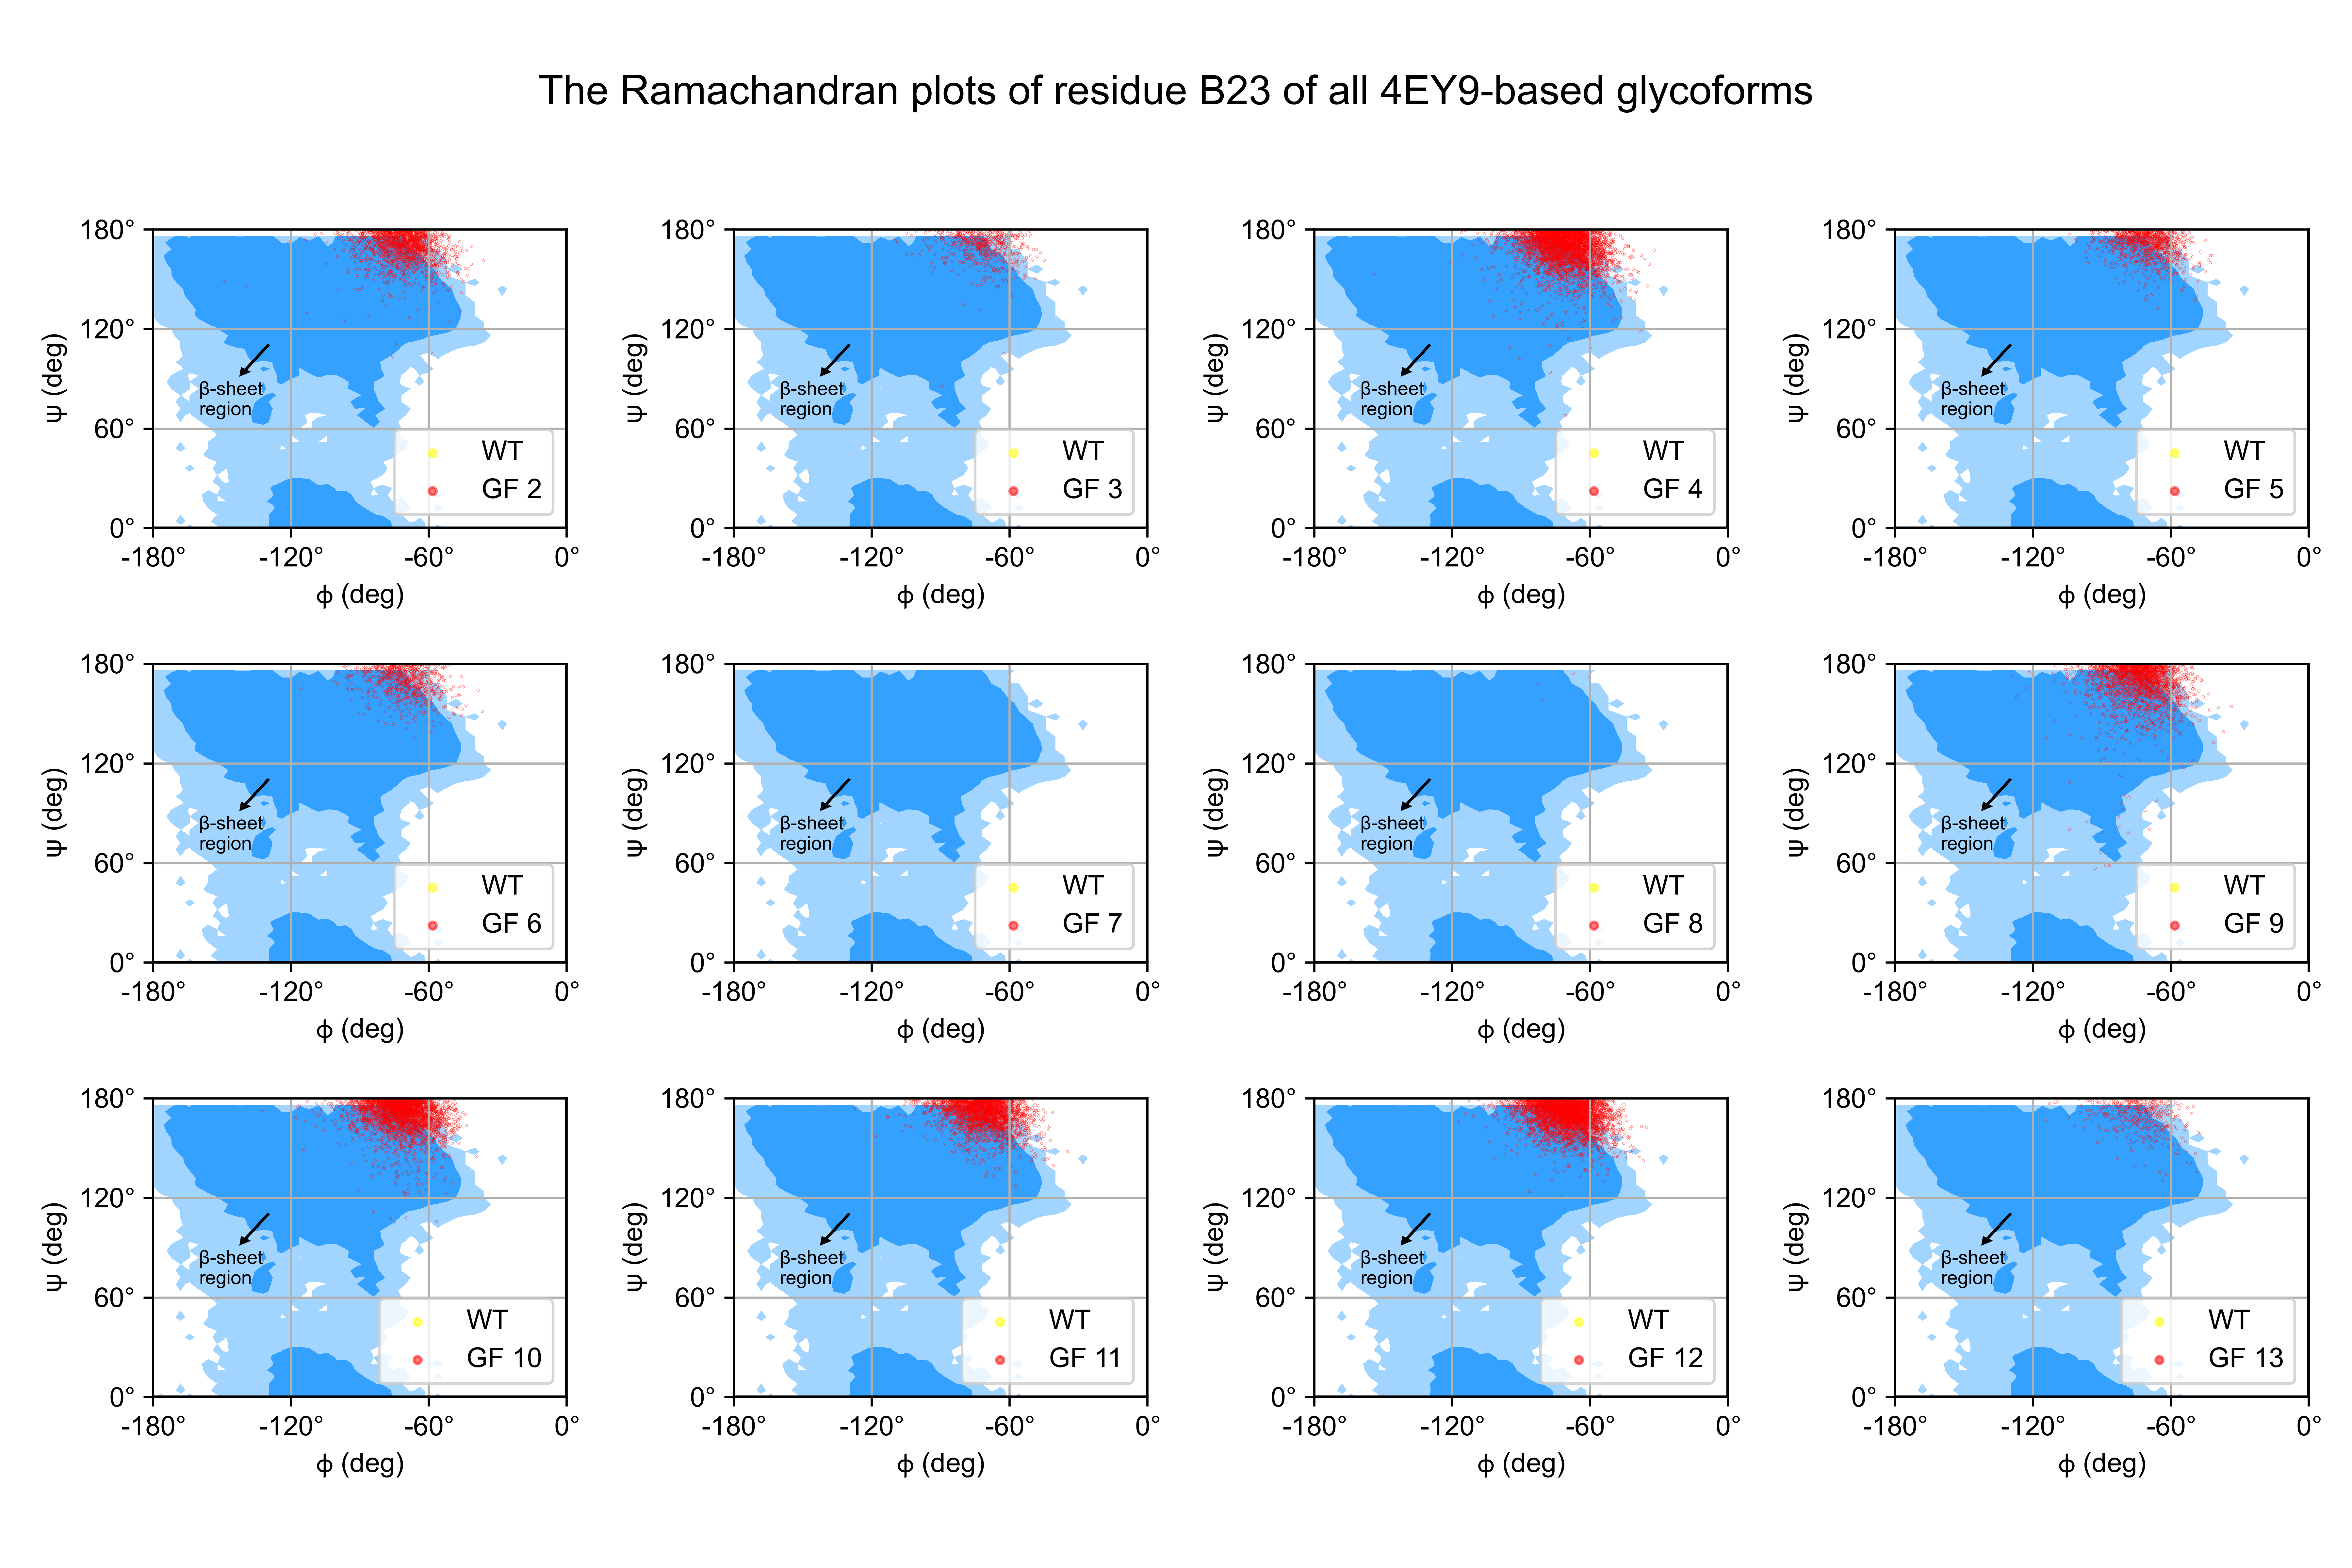
\includegraphics[width=\textwidth]{Figures/4EY9_multi_rama_plot_res_44.png}
\caption{The Ramachandran plots of residue B23 of all 4EY9-based glycoforms. The contours in the background show the allowed region in the second quadrant where the dihedral angles can reside. The deeper blue region is the $\beta$-sheet region defined by Lovell et al~\cite{lovell2003structure}.}
\end{figure}

\renewcommand{\thefigure}{S\arabic{figure}}
\begin{figure}[H]
\centering
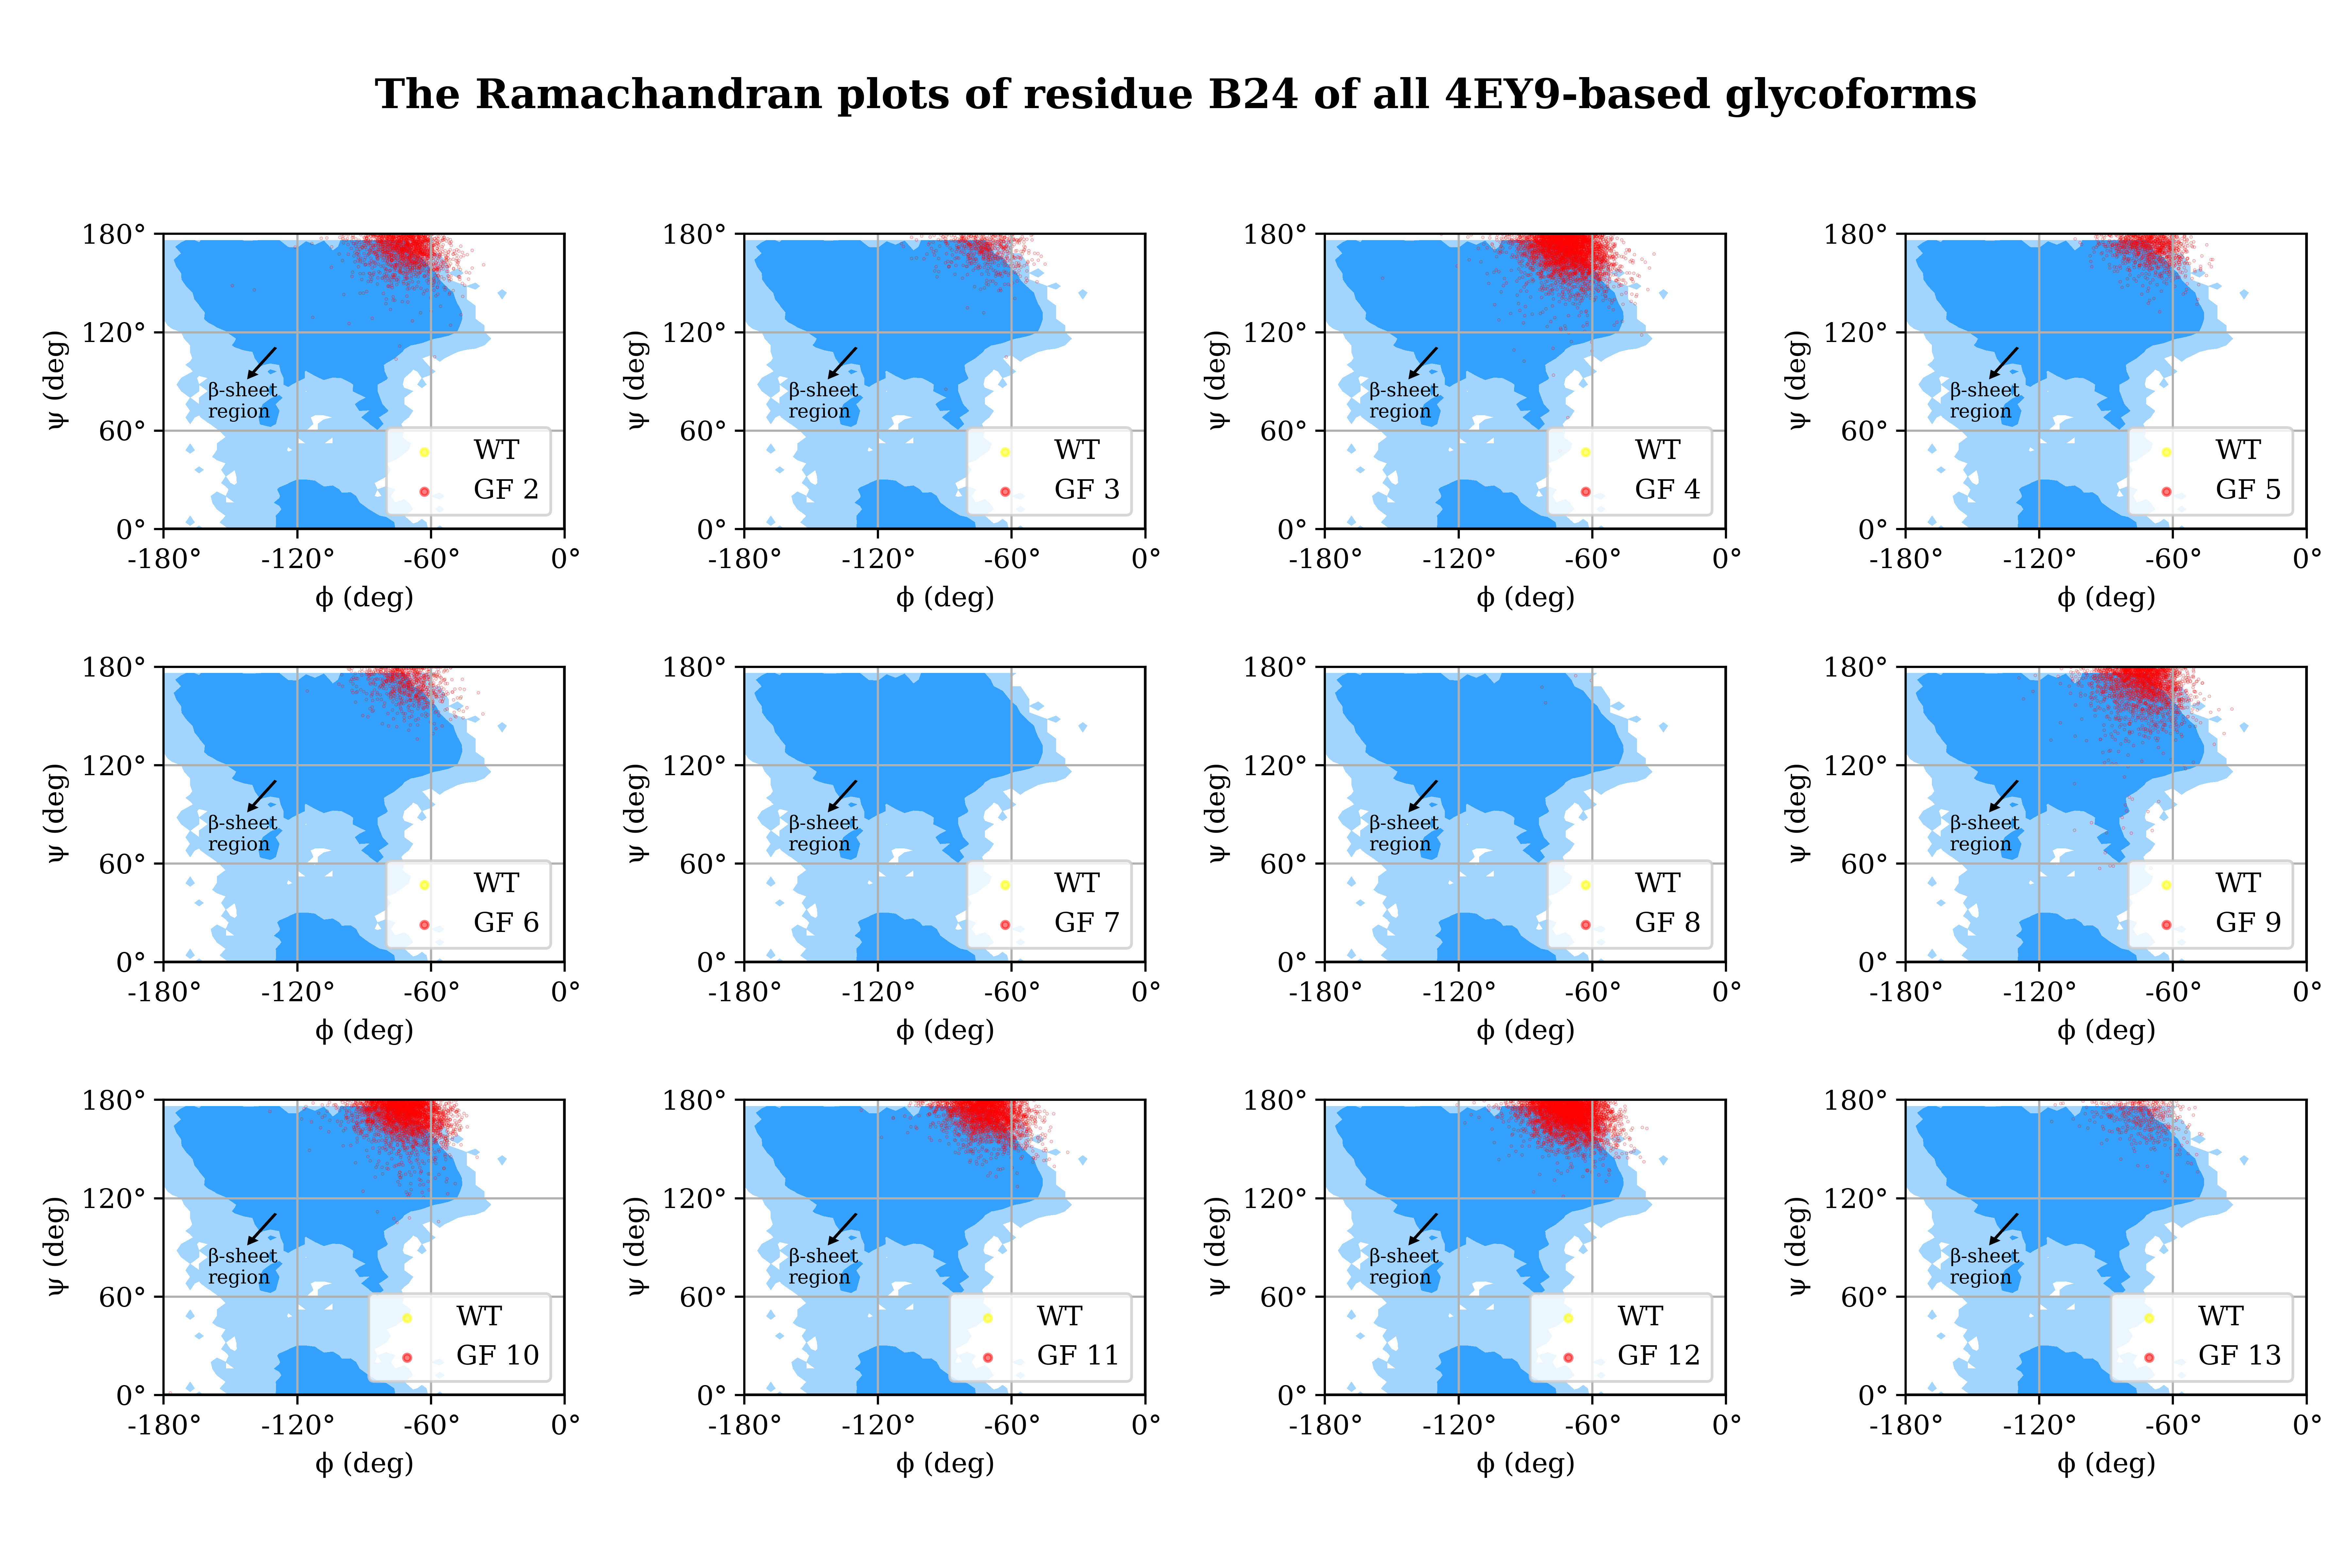
\includegraphics[width=\textwidth]{Figures/4EY9_multi_rama_plot_res_45.png}
\caption{The Ramachandran plots of residue B24 of all 4EY9-based glycoforms. The contours in the background show the allowed region in the second quadrant where the dihedral angles can reside. The deeper blue region is the $\beta$-sheet region defined by Lovell et al~\cite{lovell2003structure}.}
\end{figure}

\renewcommand{\thefigure}{S\arabic{figure}}
\begin{figure}[H]
\centering
\includegraphics[width=\textwidth]{Figures/4EY9_multi_rama_plot_res_46.png}
\caption{The Ramachandran plots of residue B25 of all 4EY9-based glycoforms. The contours in the background show the allowed region in the second quadrant where the dihedral angles can reside. The deeper blue region is the $\beta$-sheet region defined by Lovell et al~\cite{lovell2003structure}.}
\end{figure}

\renewcommand{\thefigure}{S\arabic{figure}}
\begin{figure}[H]
\centering
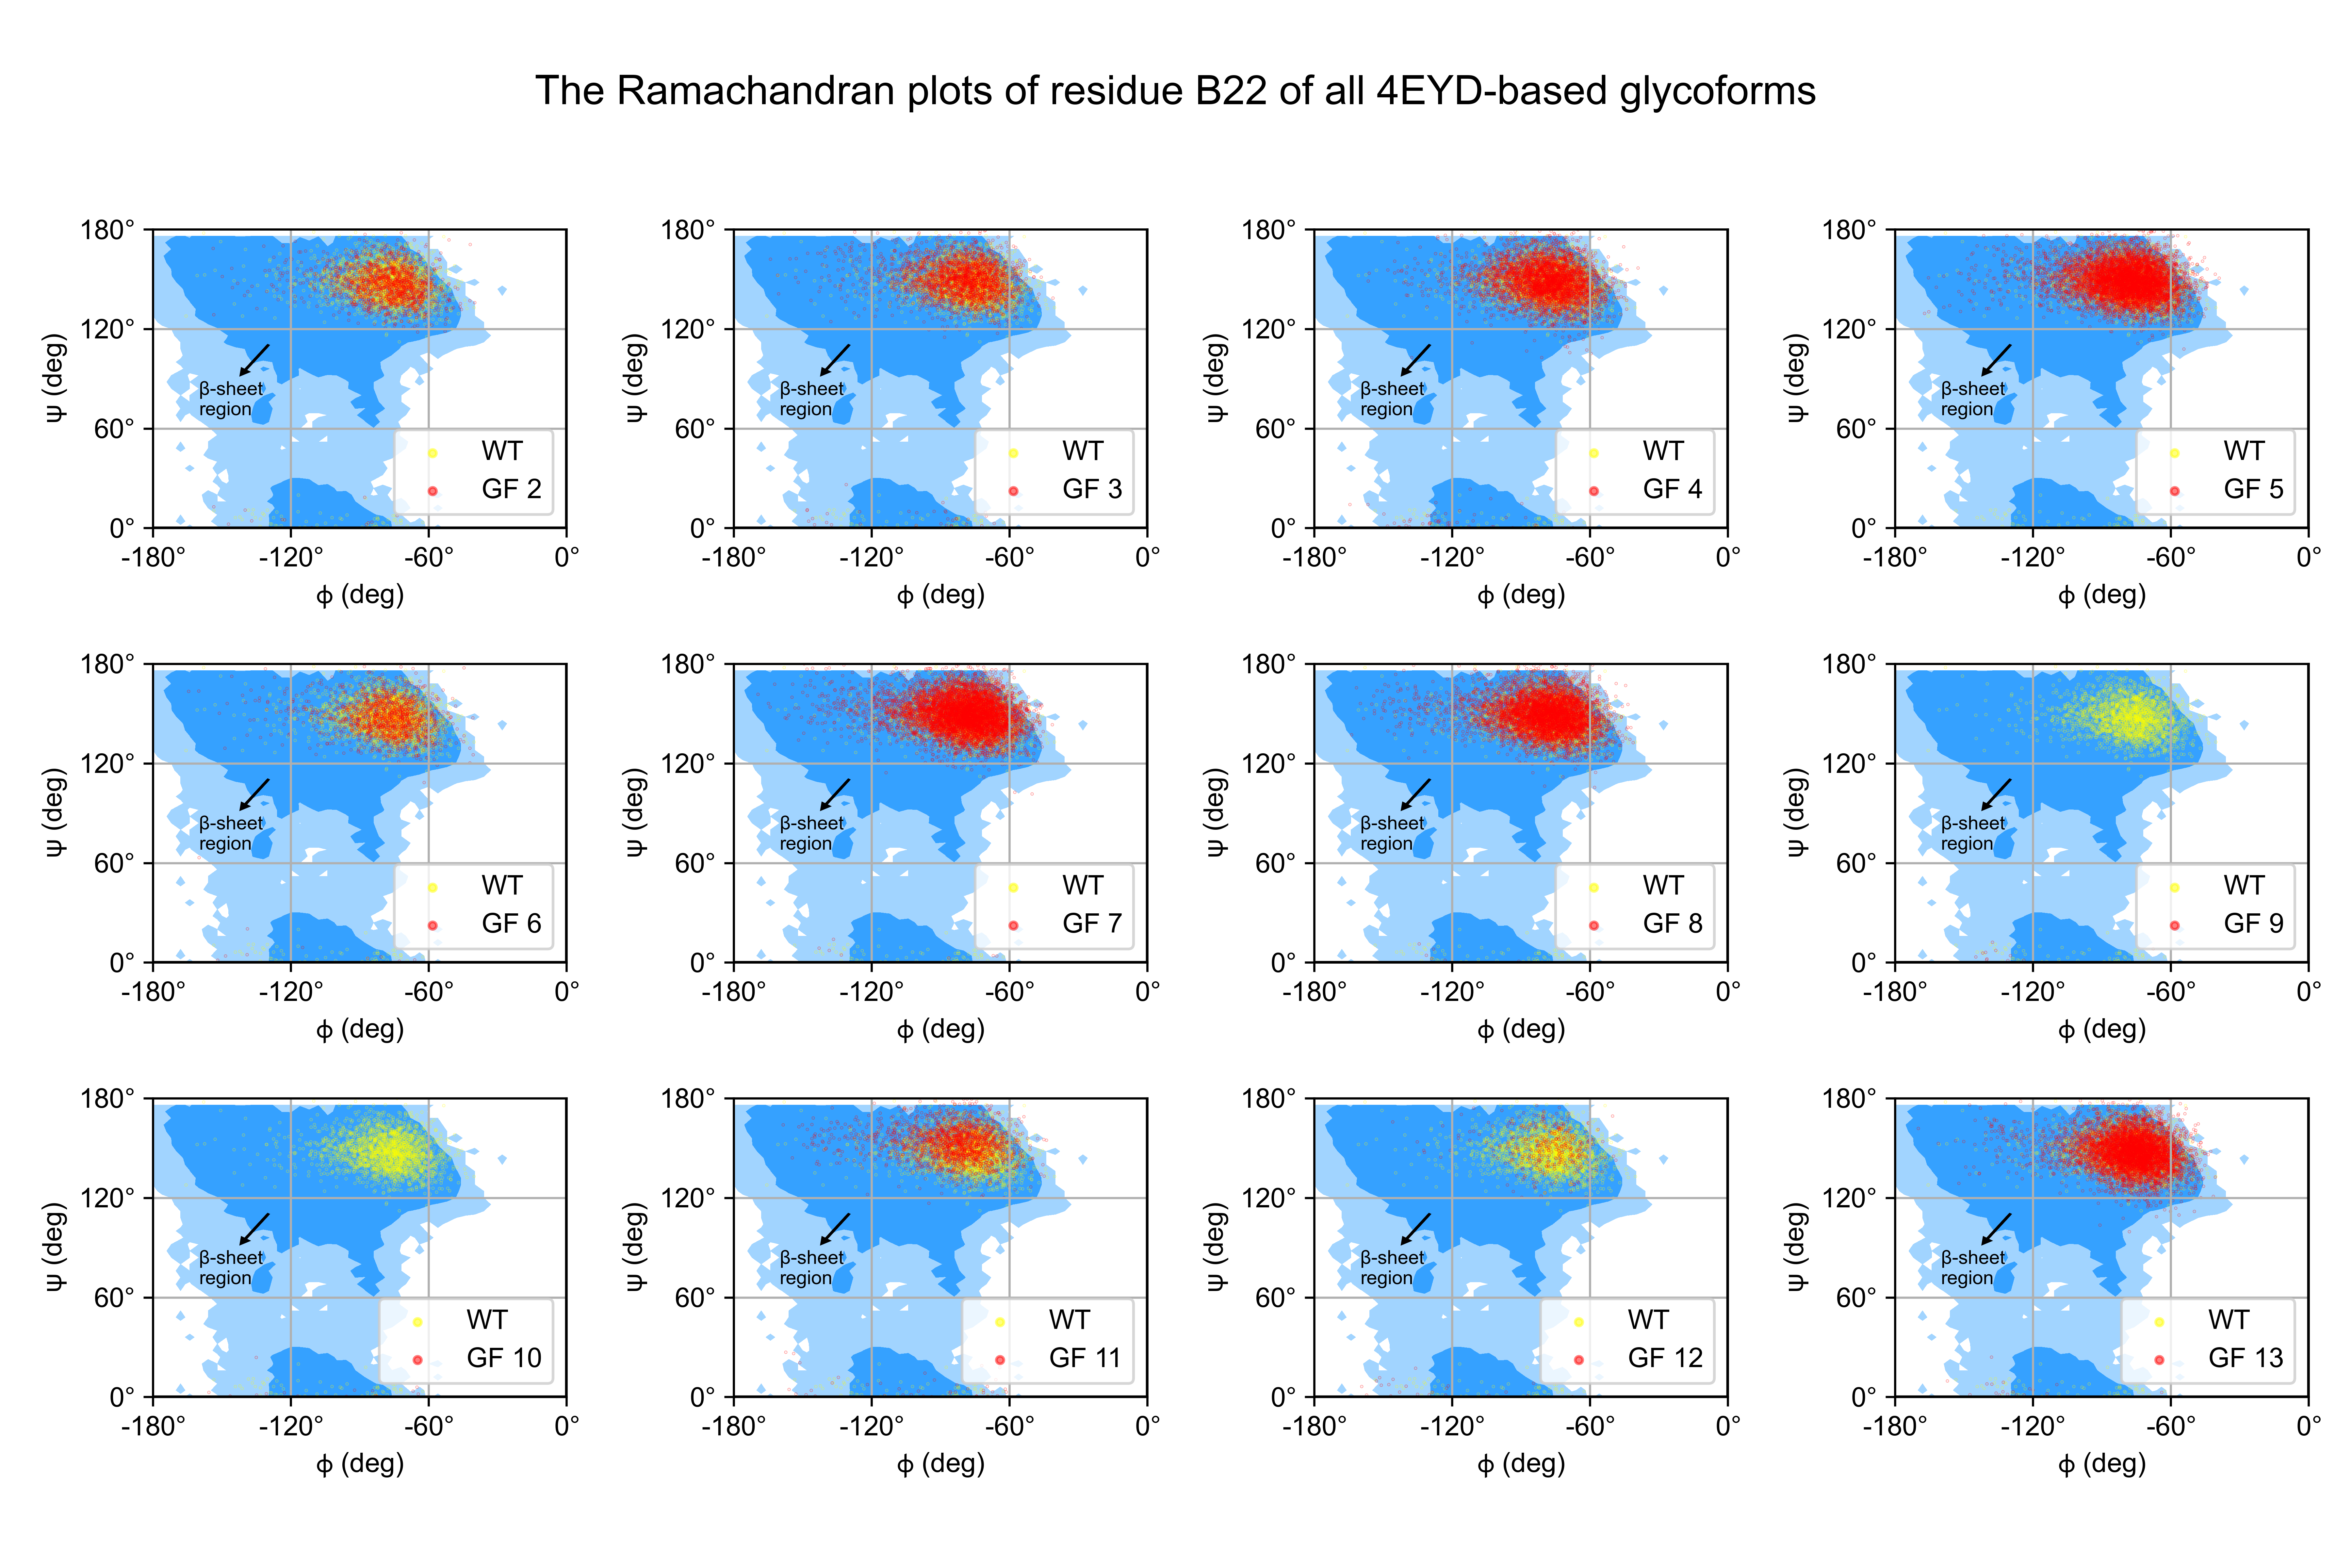
\includegraphics[width=\textwidth]{Figures/4EYD_multi_rama_plot_res_43.png}
\caption{The Ramachandran plots of residue B22 of all 4EYD-based glycoforms. The contours in the background show the allowed region in the second quadrant where the dihedral angles can reside. The deeper blue region is the $\beta$-sheet region defined by Lovell et al~\cite{lovell2003structure}.}
\end{figure}

\renewcommand{\thefigure}{S\arabic{figure}}
\begin{figure}[H]
\centering
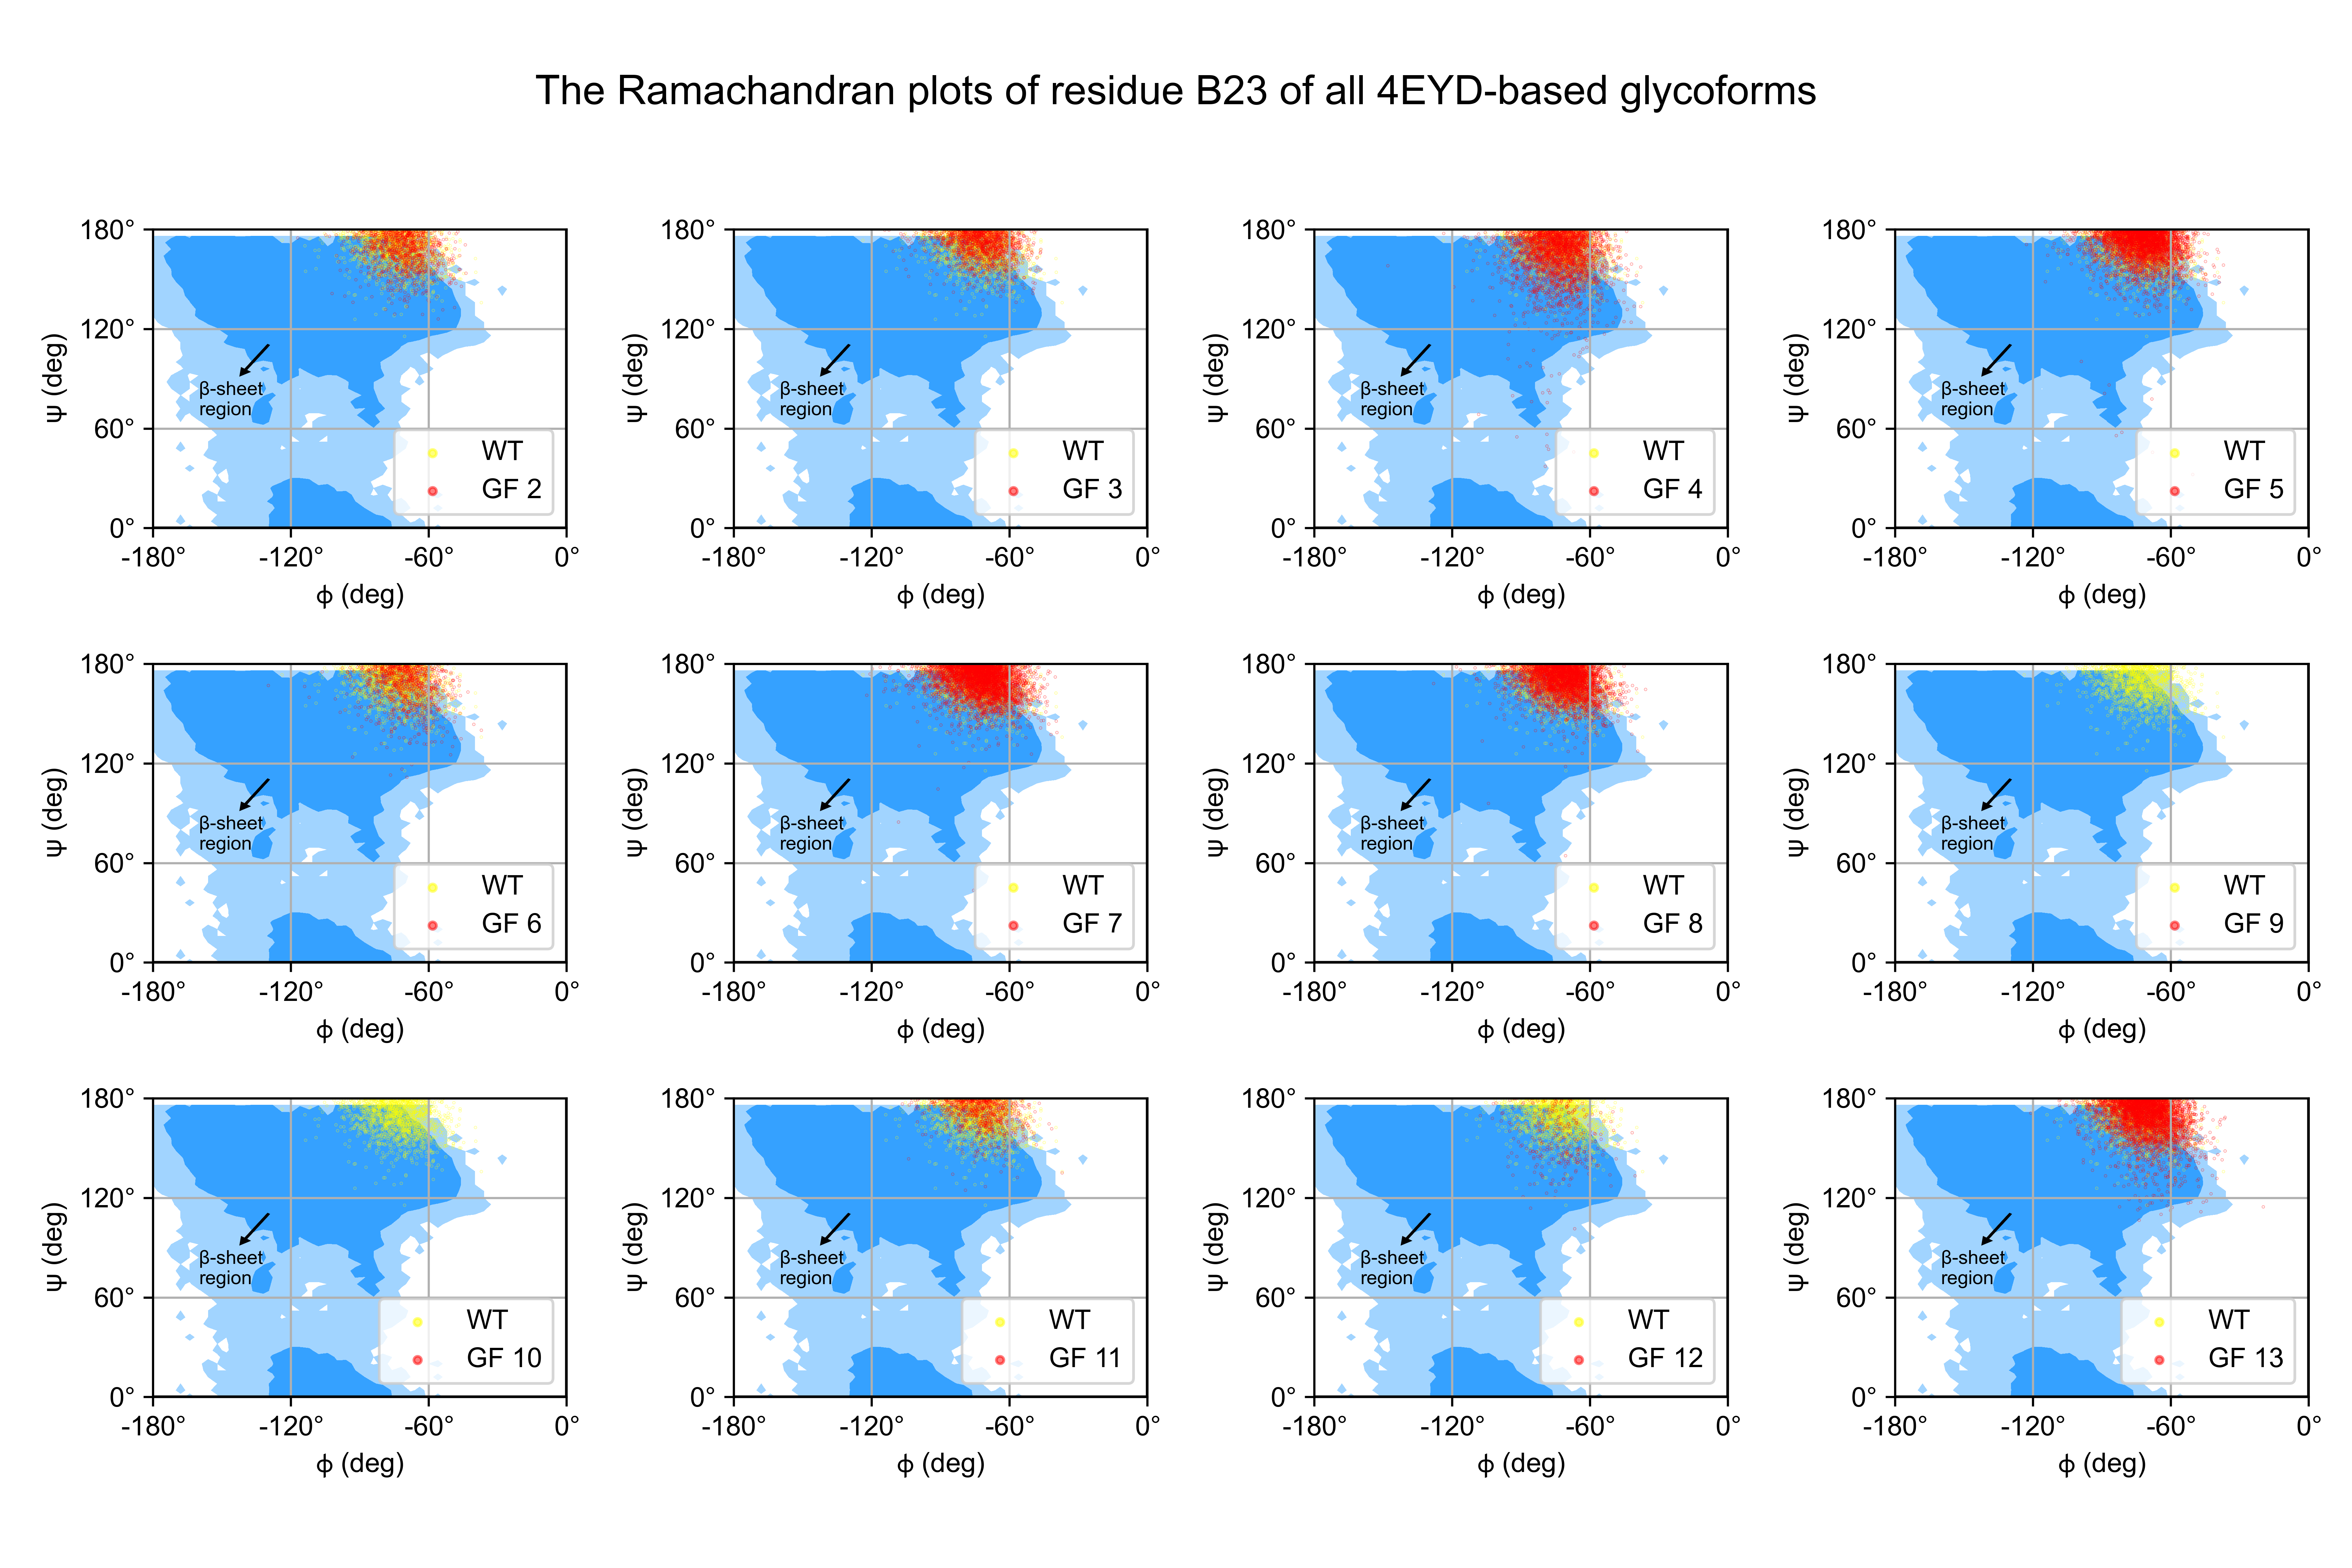
\includegraphics[width=\textwidth]{Figures/4EYD_multi_rama_plot_res_44.png}
\caption{The Ramachandran plots of residue B23 of all 4EYD-based glycoforms. The contours in the background show the allowed region in the second quadrant where the dihedral angles can reside. The deeper blue region is the $\beta$-sheet region defined by Lovell et al~\cite{lovell2003structure}.}
\end{figure}

\renewcommand{\thefigure}{S\arabic{figure}}
\begin{figure}[H]
\centering
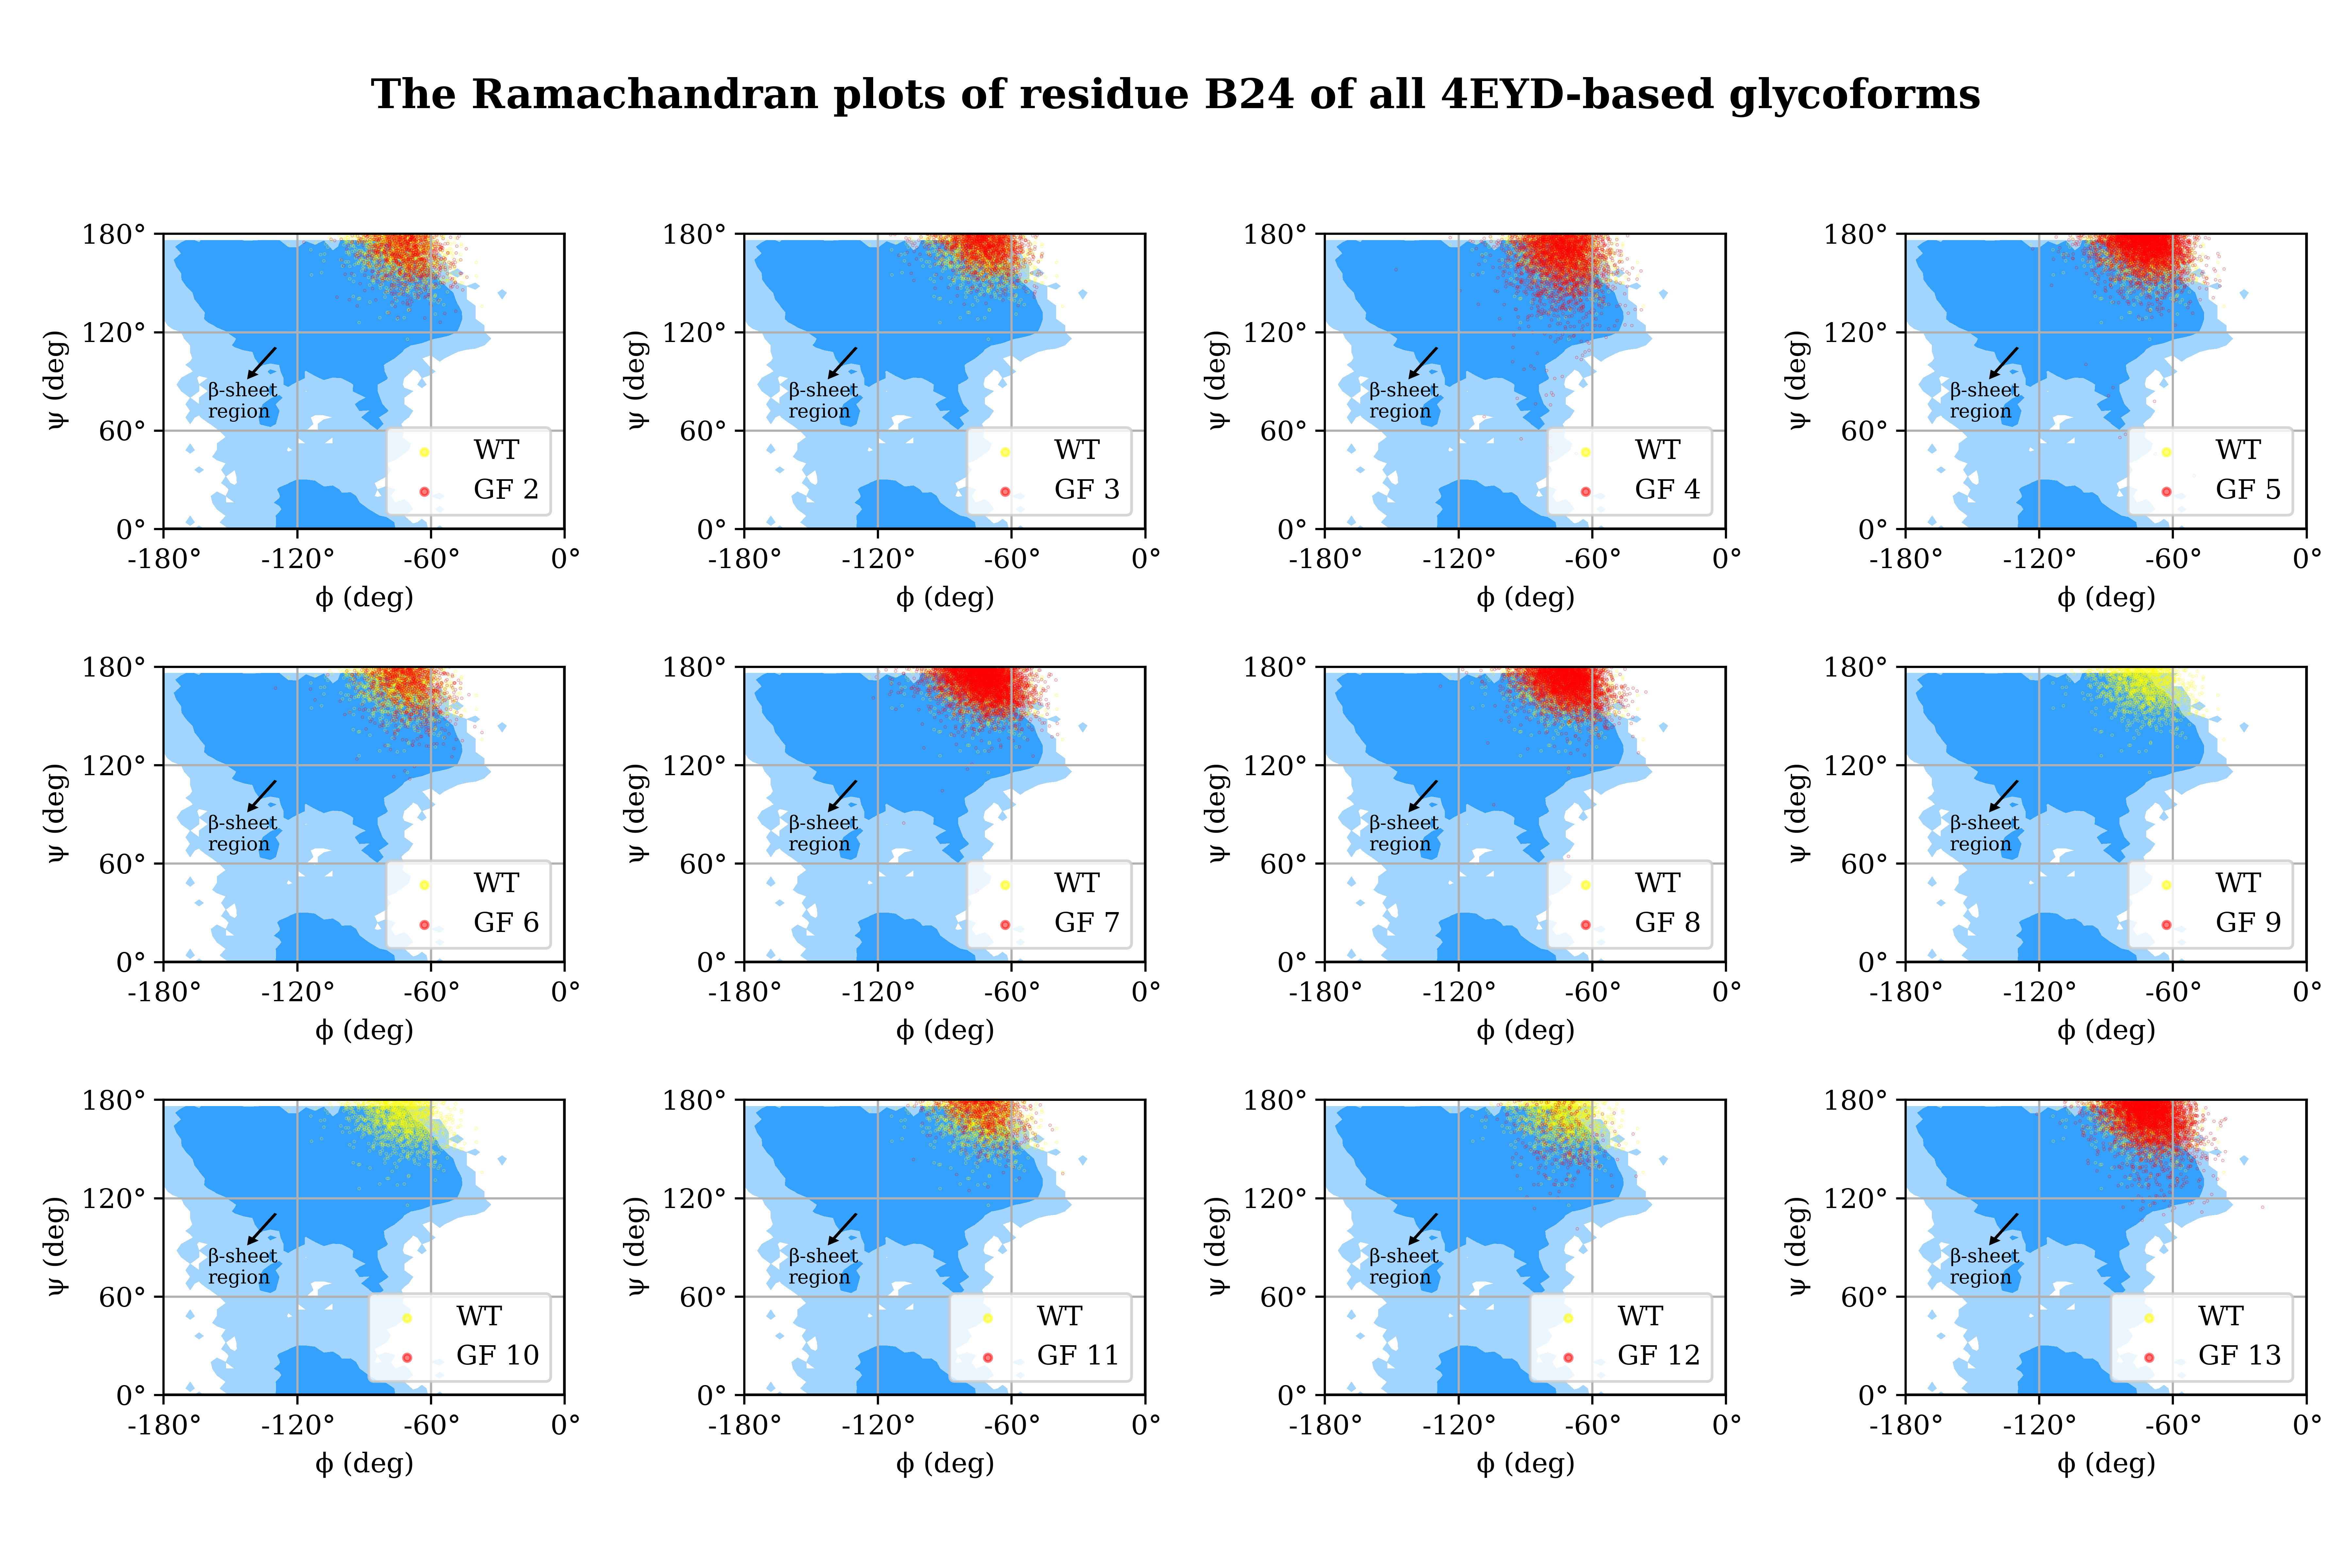
\includegraphics[width=\textwidth]{Figures/4EYD_multi_rama_plot_res_45.png}
\caption{The Ramachandran plots of residue B24 of all 4EYD-based glycoforms. The contours in the background show the allowed region in the second quadrant where the dihedral angles can reside. The deeper blue region is the $\beta$-sheet region defined by Lovell et al~\cite{lovell2003structure}.}
\end{figure}

\renewcommand{\thefigure}{S\arabic{figure}}
\begin{figure}[H]
\centering
\includegraphics[width=\textwidth]{Figures/4EYD_multi_rama_plot_res_46.png}
\caption{The Ramachandran plots of residue B25 of all 4EYD-based glycoforms. The contours in the background show the allowed region in the second quadrant where the dihedral angles can reside. The deeper blue region is the $\beta$-sheet region defined by Lovell et al~\cite{lovell2003structure}.}
\end{figure}

\bibliography{references}

\end{document}
